\documentclass[multi=tikzpicture,border=0pt]{standalone}
\usepackage{fontspec}\usepackage{tikz}\usepackage{amsmath,bm}
\setsansfont{Arial}\usetikzlibrary{arrows.meta,calc}
\definecolor{ink}{HTML}{17365D}\definecolor{beamgreen}{HTML}{2CA02C}
\definecolor{fluororange}{HTML}{FF7F0E}\definecolor{detectorblue}{HTML}{1F77B4}
\definecolor{samplegray}{HTML}{7F7F7F}\definecolor{motioncyan}{HTML}{008FA8}
\begin{document}
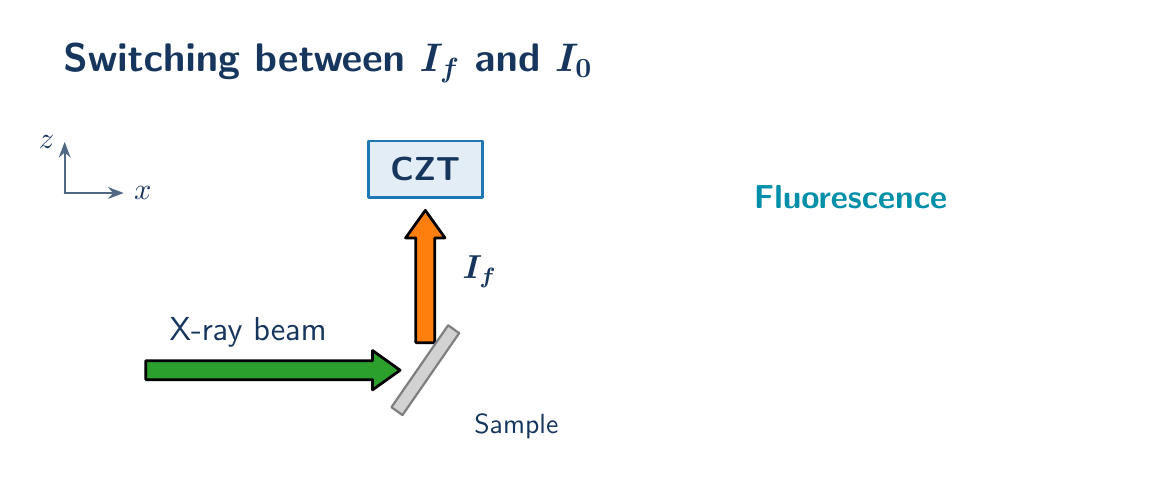
\begin{tikzpicture}[x=1cm,y=1cm,line join=round,line cap=round,
 every node/.style={font=\sffamily\fontsize{12}{14}\selectfont,text=ink},
]
\newcommand{\BeamArrow}[4]{%
  \begin{scope}
    \coordinate (beamStart) at #3;
    \coordinate (beamEnd) at #4;
    \path let \p1 = ($(beamEnd)-(beamStart)$),
      \n1 = {atan2(\y1,\x1)}, \n2 = {veclen(\x1,\y1)} in
      \pgfextra{\xdef\beamAngle{\n1}\xdef\beamLength{\n2}};
    \begin{scope}[shift={(beamStart)},rotate=\beamAngle]
      \path[fill=#1,draw=black,opacity=#2,line width=.35mm,line join=round]
        (0,-1.2mm) -- (\beamLength-3.5mm,-1.2mm)
        -- (\beamLength-3.5mm,-2.5mm) -- (\beamLength,0)
        -- (\beamLength-3.5mm,2.5mm) -- (\beamLength-3.5mm,1.2mm)
        -- (0,1.2mm) -- cycle;
    \end{scope}
  \end{scope}
}
\path[use as bounding box] (-1.05,-1.25) rectangle (12.8878,4.35);
\node[anchor=west,font=\sffamily\bfseries\fontsize{14}{17}\selectfont] at (-.72,3.9) {Switching between $\bm{I_f}$ and $\bm{I_0}$};
\draw[ink!75,line width=.8pt,-{Stealth[length=2mm]}] (-.58,2.25) -- (.17,2.25) node[anchor=west,font=\sffamily\fontsize{11}{13}\selectfont] {$x$};
\draw[ink!75,line width=.8pt,-{Stealth[length=2mm]}] (-.58,2.25) -- (-.58,2.9) node[anchor=east,font=\sffamily\fontsize{11}{13}\selectfont] {$z$};
\BeamArrow{beamgreen}{1.0000}{(.45,0)}{(3.68,0)}
\node at (1.75,.48) {X-ray beam};
\BeamArrow{beamgreen}{0.0000}{(.45,0)}{(5.98,0)}
\BeamArrow{fluororange}{1.0000}{(4,.35)}{(4,2.03)}
\node[opacity=1.0000,anchor=west] at (4.35,1.25) {$\bm{I_f}$};
\node[opacity=0.0000] at (5.25,.48) {$\bm{I_0}$};
\begin{scope}[shift={(4,0.0000)}]
\path[draw=samplegray,fill=samplegray!35,line width=.8pt] (-.43,-.47) -- (-.29,-.57) -- (.43,.47) -- (.29,.57) -- cycle;
\end{scope}
\node[anchor=west,font=\sffamily\fontsize{10}{12}\selectfont] at (4.5,-0.7200) {Sample};
\begin{scope}[shift={(4.0000,2.5500)},rotate=-0.0000,transform shape]
\node[draw=detectorblue,fill=detectorblue!13,line width=1pt,minimum width=1.45cm,minimum height=.72cm,inner sep=2pt,font=\sffamily\bfseries\fontsize{13}{15}\selectfont] {CZT};
\end{scope}
\node[opacity=1.0000,font=\sffamily\bfseries\fontsize{13}{15}\selectfont,text=motioncyan] at (9.4,2.2) {Fluorescence};
\node[opacity=0.0000,font=\sffamily\bfseries\fontsize{13}{15}\selectfont,text=motioncyan] at (9.4,2.2) {Incident beam};
\end{tikzpicture}
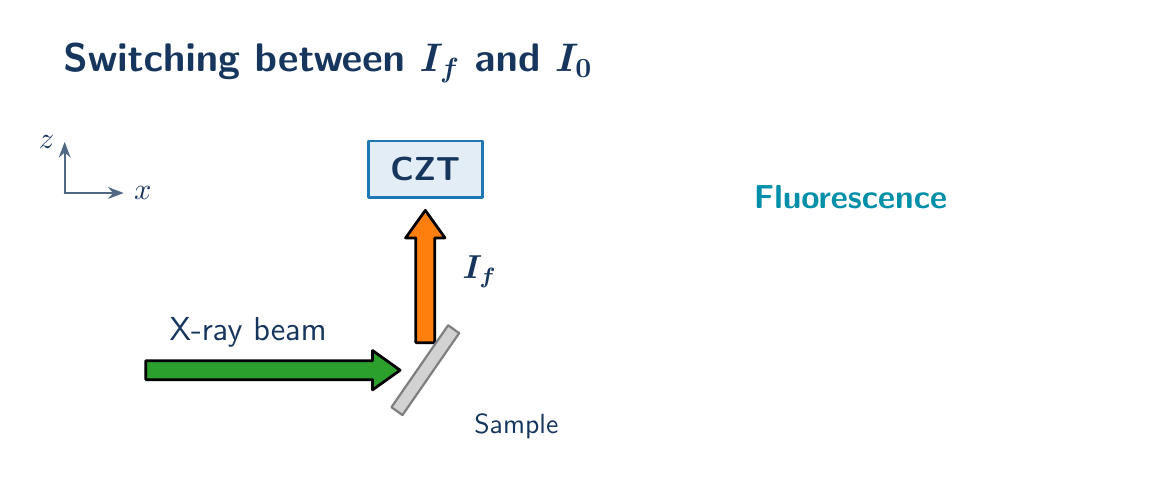
\begin{tikzpicture}[x=1cm,y=1cm,line join=round,line cap=round,
 every node/.style={font=\sffamily\fontsize{12}{14}\selectfont,text=ink},
]
\newcommand{\BeamArrow}[4]{%
  \begin{scope}
    \coordinate (beamStart) at #3;
    \coordinate (beamEnd) at #4;
    \path let \p1 = ($(beamEnd)-(beamStart)$),
      \n1 = {atan2(\y1,\x1)}, \n2 = {veclen(\x1,\y1)} in
      \pgfextra{\xdef\beamAngle{\n1}\xdef\beamLength{\n2}};
    \begin{scope}[shift={(beamStart)},rotate=\beamAngle]
      \path[fill=#1,draw=black,opacity=#2,line width=.35mm,line join=round]
        (0,-1.2mm) -- (\beamLength-3.5mm,-1.2mm)
        -- (\beamLength-3.5mm,-2.5mm) -- (\beamLength,0)
        -- (\beamLength-3.5mm,2.5mm) -- (\beamLength-3.5mm,1.2mm)
        -- (0,1.2mm) -- cycle;
    \end{scope}
  \end{scope}
}
\path[use as bounding box] (-1.05,-1.25) rectangle (12.8878,4.35);
\node[anchor=west,font=\sffamily\bfseries\fontsize{14}{17}\selectfont] at (-.72,3.9) {Switching between $\bm{I_f}$ and $\bm{I_0}$};
\draw[ink!75,line width=.8pt,-{Stealth[length=2mm]}] (-.58,2.25) -- (.17,2.25) node[anchor=west,font=\sffamily\fontsize{11}{13}\selectfont] {$x$};
\draw[ink!75,line width=.8pt,-{Stealth[length=2mm]}] (-.58,2.25) -- (-.58,2.9) node[anchor=east,font=\sffamily\fontsize{11}{13}\selectfont] {$z$};
\BeamArrow{beamgreen}{1.0000}{(.45,0)}{(3.68,0)}
\node at (1.75,.48) {X-ray beam};
\BeamArrow{beamgreen}{0.0000}{(.45,0)}{(5.98,0)}
\BeamArrow{fluororange}{1.0000}{(4,.35)}{(4,2.03)}
\node[opacity=1.0000,anchor=west] at (4.35,1.25) {$\bm{I_f}$};
\node[opacity=0.0000] at (5.25,.48) {$\bm{I_0}$};
\begin{scope}[shift={(4,0.0000)}]
\path[draw=samplegray,fill=samplegray!35,line width=.8pt] (-.43,-.47) -- (-.29,-.57) -- (.43,.47) -- (.29,.57) -- cycle;
\end{scope}
\node[anchor=west,font=\sffamily\fontsize{10}{12}\selectfont] at (4.5,-0.7200) {Sample};
\begin{scope}[shift={(4.0000,2.5500)},rotate=-0.0000,transform shape]
\node[draw=detectorblue,fill=detectorblue!13,line width=1pt,minimum width=1.45cm,minimum height=.72cm,inner sep=2pt,font=\sffamily\bfseries\fontsize{13}{15}\selectfont] {CZT};
\end{scope}
\node[opacity=1.0000,font=\sffamily\bfseries\fontsize{13}{15}\selectfont,text=motioncyan] at (9.4,2.2) {Fluorescence};
\node[opacity=0.0000,font=\sffamily\bfseries\fontsize{13}{15}\selectfont,text=motioncyan] at (9.4,2.2) {Incident beam};
\end{tikzpicture}
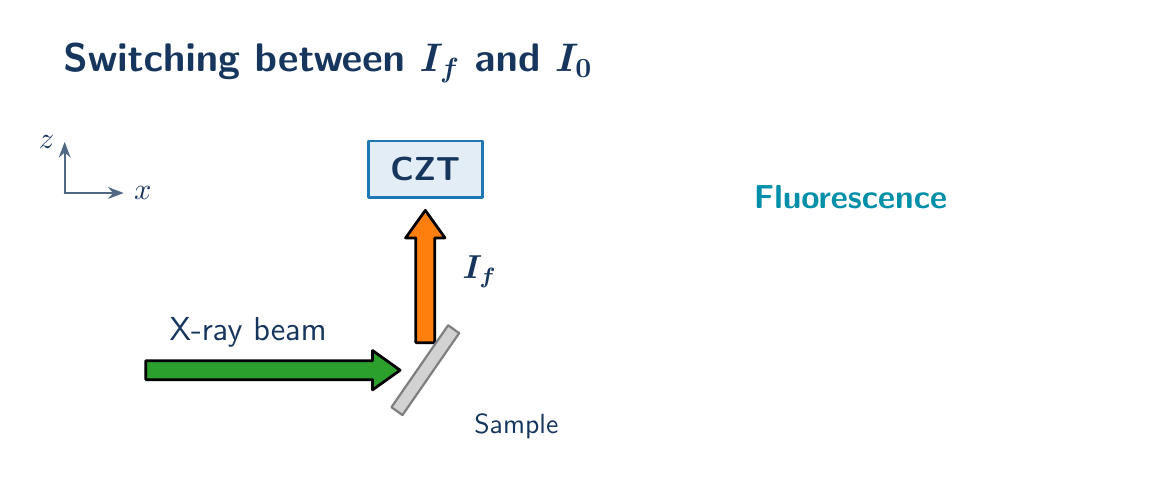
\begin{tikzpicture}[x=1cm,y=1cm,line join=round,line cap=round,
 every node/.style={font=\sffamily\fontsize{12}{14}\selectfont,text=ink},
]
\newcommand{\BeamArrow}[4]{%
  \begin{scope}
    \coordinate (beamStart) at #3;
    \coordinate (beamEnd) at #4;
    \path let \p1 = ($(beamEnd)-(beamStart)$),
      \n1 = {atan2(\y1,\x1)}, \n2 = {veclen(\x1,\y1)} in
      \pgfextra{\xdef\beamAngle{\n1}\xdef\beamLength{\n2}};
    \begin{scope}[shift={(beamStart)},rotate=\beamAngle]
      \path[fill=#1,draw=black,opacity=#2,line width=.35mm,line join=round]
        (0,-1.2mm) -- (\beamLength-3.5mm,-1.2mm)
        -- (\beamLength-3.5mm,-2.5mm) -- (\beamLength,0)
        -- (\beamLength-3.5mm,2.5mm) -- (\beamLength-3.5mm,1.2mm)
        -- (0,1.2mm) -- cycle;
    \end{scope}
  \end{scope}
}
\path[use as bounding box] (-1.05,-1.25) rectangle (12.8878,4.35);
\node[anchor=west,font=\sffamily\bfseries\fontsize{14}{17}\selectfont] at (-.72,3.9) {Switching between $\bm{I_f}$ and $\bm{I_0}$};
\draw[ink!75,line width=.8pt,-{Stealth[length=2mm]}] (-.58,2.25) -- (.17,2.25) node[anchor=west,font=\sffamily\fontsize{11}{13}\selectfont] {$x$};
\draw[ink!75,line width=.8pt,-{Stealth[length=2mm]}] (-.58,2.25) -- (-.58,2.9) node[anchor=east,font=\sffamily\fontsize{11}{13}\selectfont] {$z$};
\BeamArrow{beamgreen}{1.0000}{(.45,0)}{(3.68,0)}
\node at (1.75,.48) {X-ray beam};
\BeamArrow{beamgreen}{0.0000}{(.45,0)}{(5.98,0)}
\BeamArrow{fluororange}{1.0000}{(4,.35)}{(4,2.03)}
\node[opacity=1.0000,anchor=west] at (4.35,1.25) {$\bm{I_f}$};
\node[opacity=0.0000] at (5.25,.48) {$\bm{I_0}$};
\begin{scope}[shift={(4,0.0000)}]
\path[draw=samplegray,fill=samplegray!35,line width=.8pt] (-.43,-.47) -- (-.29,-.57) -- (.43,.47) -- (.29,.57) -- cycle;
\end{scope}
\node[anchor=west,font=\sffamily\fontsize{10}{12}\selectfont] at (4.5,-0.7200) {Sample};
\begin{scope}[shift={(4.0000,2.5500)},rotate=-0.0000,transform shape]
\node[draw=detectorblue,fill=detectorblue!13,line width=1pt,minimum width=1.45cm,minimum height=.72cm,inner sep=2pt,font=\sffamily\bfseries\fontsize{13}{15}\selectfont] {CZT};
\end{scope}
\node[opacity=1.0000,font=\sffamily\bfseries\fontsize{13}{15}\selectfont,text=motioncyan] at (9.4,2.2) {Fluorescence};
\node[opacity=0.0000,font=\sffamily\bfseries\fontsize{13}{15}\selectfont,text=motioncyan] at (9.4,2.2) {Incident beam};
\end{tikzpicture}
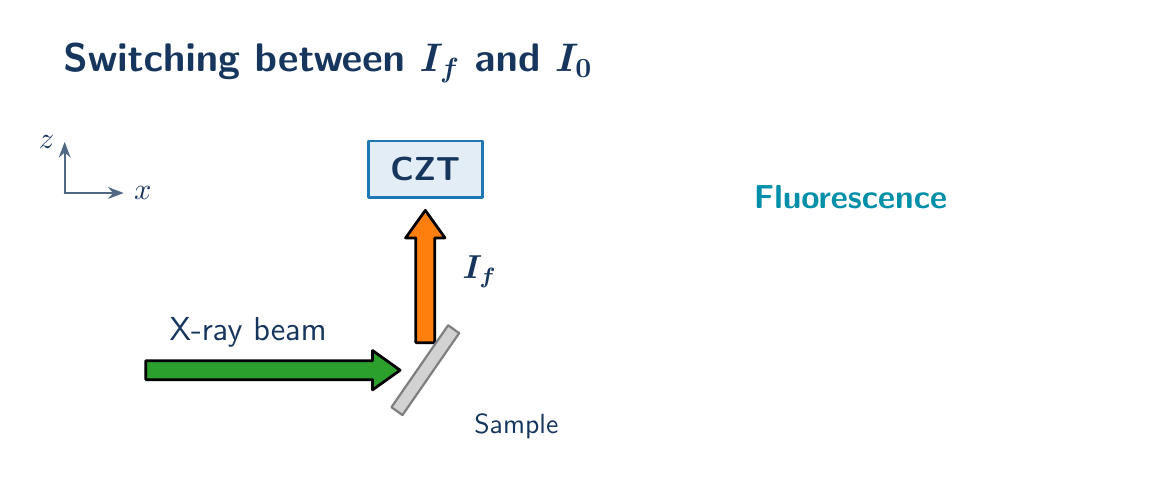
\begin{tikzpicture}[x=1cm,y=1cm,line join=round,line cap=round,
 every node/.style={font=\sffamily\fontsize{12}{14}\selectfont,text=ink},
]
\newcommand{\BeamArrow}[4]{%
  \begin{scope}
    \coordinate (beamStart) at #3;
    \coordinate (beamEnd) at #4;
    \path let \p1 = ($(beamEnd)-(beamStart)$),
      \n1 = {atan2(\y1,\x1)}, \n2 = {veclen(\x1,\y1)} in
      \pgfextra{\xdef\beamAngle{\n1}\xdef\beamLength{\n2}};
    \begin{scope}[shift={(beamStart)},rotate=\beamAngle]
      \path[fill=#1,draw=black,opacity=#2,line width=.35mm,line join=round]
        (0,-1.2mm) -- (\beamLength-3.5mm,-1.2mm)
        -- (\beamLength-3.5mm,-2.5mm) -- (\beamLength,0)
        -- (\beamLength-3.5mm,2.5mm) -- (\beamLength-3.5mm,1.2mm)
        -- (0,1.2mm) -- cycle;
    \end{scope}
  \end{scope}
}
\path[use as bounding box] (-1.05,-1.25) rectangle (12.8878,4.35);
\node[anchor=west,font=\sffamily\bfseries\fontsize{14}{17}\selectfont] at (-.72,3.9) {Switching between $\bm{I_f}$ and $\bm{I_0}$};
\draw[ink!75,line width=.8pt,-{Stealth[length=2mm]}] (-.58,2.25) -- (.17,2.25) node[anchor=west,font=\sffamily\fontsize{11}{13}\selectfont] {$x$};
\draw[ink!75,line width=.8pt,-{Stealth[length=2mm]}] (-.58,2.25) -- (-.58,2.9) node[anchor=east,font=\sffamily\fontsize{11}{13}\selectfont] {$z$};
\BeamArrow{beamgreen}{1.0000}{(.45,0)}{(3.68,0)}
\node at (1.75,.48) {X-ray beam};
\BeamArrow{beamgreen}{0.0000}{(.45,0)}{(5.98,0)}
\BeamArrow{fluororange}{1.0000}{(4,.35)}{(4,2.03)}
\node[opacity=1.0000,anchor=west] at (4.35,1.25) {$\bm{I_f}$};
\node[opacity=0.0000] at (5.25,.48) {$\bm{I_0}$};
\begin{scope}[shift={(4,0.0000)}]
\path[draw=samplegray,fill=samplegray!35,line width=.8pt] (-.43,-.47) -- (-.29,-.57) -- (.43,.47) -- (.29,.57) -- cycle;
\end{scope}
\node[anchor=west,font=\sffamily\fontsize{10}{12}\selectfont] at (4.5,-0.7200) {Sample};
\begin{scope}[shift={(4.0000,2.5500)},rotate=-0.0000,transform shape]
\node[draw=detectorblue,fill=detectorblue!13,line width=1pt,minimum width=1.45cm,minimum height=.72cm,inner sep=2pt,font=\sffamily\bfseries\fontsize{13}{15}\selectfont] {CZT};
\end{scope}
\node[opacity=1.0000,font=\sffamily\bfseries\fontsize{13}{15}\selectfont,text=motioncyan] at (9.4,2.2) {Fluorescence};
\node[opacity=0.0000,font=\sffamily\bfseries\fontsize{13}{15}\selectfont,text=motioncyan] at (9.4,2.2) {Incident beam};
\end{tikzpicture}
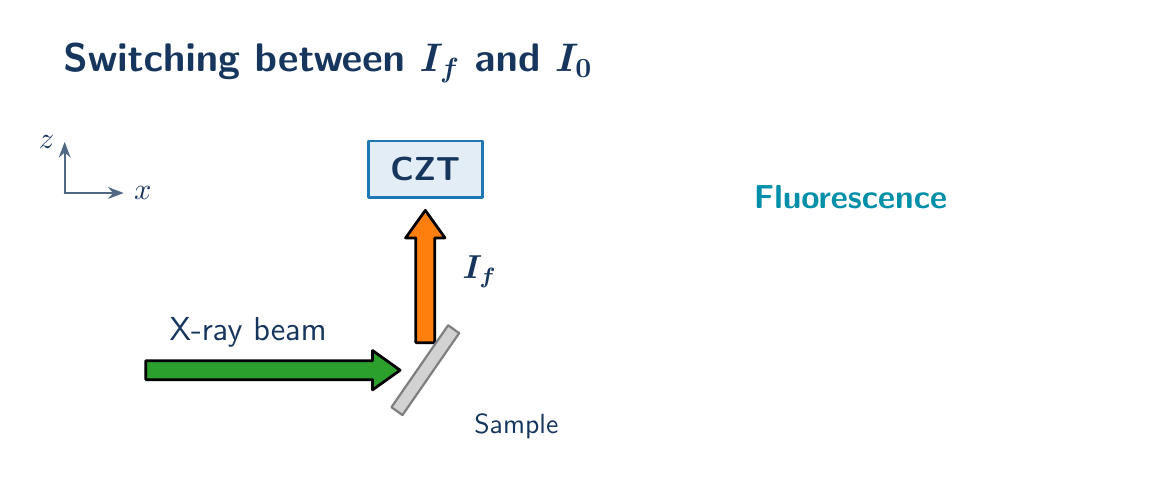
\begin{tikzpicture}[x=1cm,y=1cm,line join=round,line cap=round,
 every node/.style={font=\sffamily\fontsize{12}{14}\selectfont,text=ink},
]
\newcommand{\BeamArrow}[4]{%
  \begin{scope}
    \coordinate (beamStart) at #3;
    \coordinate (beamEnd) at #4;
    \path let \p1 = ($(beamEnd)-(beamStart)$),
      \n1 = {atan2(\y1,\x1)}, \n2 = {veclen(\x1,\y1)} in
      \pgfextra{\xdef\beamAngle{\n1}\xdef\beamLength{\n2}};
    \begin{scope}[shift={(beamStart)},rotate=\beamAngle]
      \path[fill=#1,draw=black,opacity=#2,line width=.35mm,line join=round]
        (0,-1.2mm) -- (\beamLength-3.5mm,-1.2mm)
        -- (\beamLength-3.5mm,-2.5mm) -- (\beamLength,0)
        -- (\beamLength-3.5mm,2.5mm) -- (\beamLength-3.5mm,1.2mm)
        -- (0,1.2mm) -- cycle;
    \end{scope}
  \end{scope}
}
\path[use as bounding box] (-1.05,-1.25) rectangle (12.8878,4.35);
\node[anchor=west,font=\sffamily\bfseries\fontsize{14}{17}\selectfont] at (-.72,3.9) {Switching between $\bm{I_f}$ and $\bm{I_0}$};
\draw[ink!75,line width=.8pt,-{Stealth[length=2mm]}] (-.58,2.25) -- (.17,2.25) node[anchor=west,font=\sffamily\fontsize{11}{13}\selectfont] {$x$};
\draw[ink!75,line width=.8pt,-{Stealth[length=2mm]}] (-.58,2.25) -- (-.58,2.9) node[anchor=east,font=\sffamily\fontsize{11}{13}\selectfont] {$z$};
\BeamArrow{beamgreen}{1.0000}{(.45,0)}{(3.68,0)}
\node at (1.75,.48) {X-ray beam};
\BeamArrow{beamgreen}{0.0000}{(.45,0)}{(5.98,0)}
\BeamArrow{fluororange}{1.0000}{(4,.35)}{(4,2.03)}
\node[opacity=1.0000,anchor=west] at (4.35,1.25) {$\bm{I_f}$};
\node[opacity=0.0000] at (5.25,.48) {$\bm{I_0}$};
\begin{scope}[shift={(4,0.0000)}]
\path[draw=samplegray,fill=samplegray!35,line width=.8pt] (-.43,-.47) -- (-.29,-.57) -- (.43,.47) -- (.29,.57) -- cycle;
\end{scope}
\node[anchor=west,font=\sffamily\fontsize{10}{12}\selectfont] at (4.5,-0.7200) {Sample};
\begin{scope}[shift={(4.0000,2.5500)},rotate=-0.0000,transform shape]
\node[draw=detectorblue,fill=detectorblue!13,line width=1pt,minimum width=1.45cm,minimum height=.72cm,inner sep=2pt,font=\sffamily\bfseries\fontsize{13}{15}\selectfont] {CZT};
\end{scope}
\node[opacity=1.0000,font=\sffamily\bfseries\fontsize{13}{15}\selectfont,text=motioncyan] at (9.4,2.2) {Fluorescence};
\node[opacity=0.0000,font=\sffamily\bfseries\fontsize{13}{15}\selectfont,text=motioncyan] at (9.4,2.2) {Incident beam};
\end{tikzpicture}
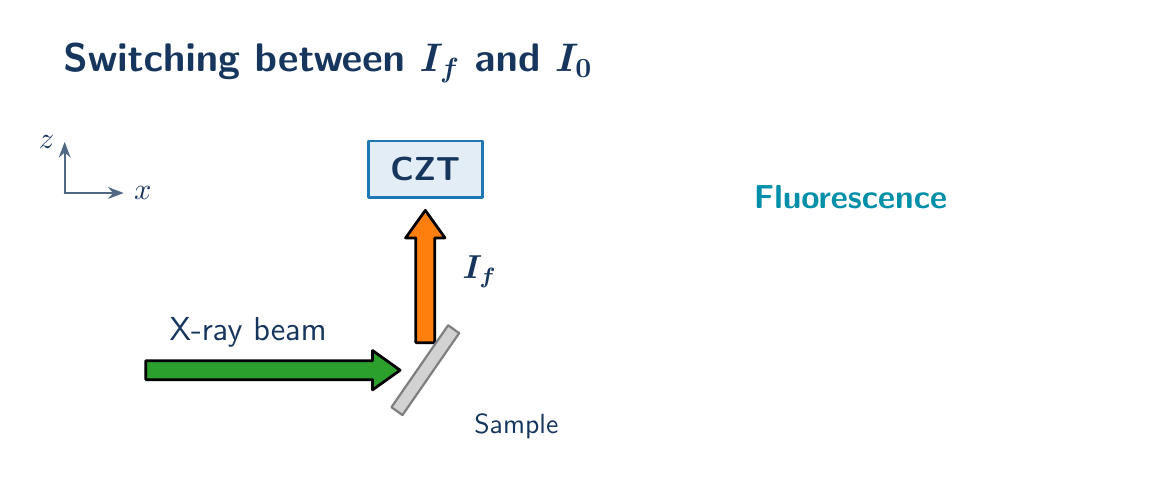
\begin{tikzpicture}[x=1cm,y=1cm,line join=round,line cap=round,
 every node/.style={font=\sffamily\fontsize{12}{14}\selectfont,text=ink},
]
\newcommand{\BeamArrow}[4]{%
  \begin{scope}
    \coordinate (beamStart) at #3;
    \coordinate (beamEnd) at #4;
    \path let \p1 = ($(beamEnd)-(beamStart)$),
      \n1 = {atan2(\y1,\x1)}, \n2 = {veclen(\x1,\y1)} in
      \pgfextra{\xdef\beamAngle{\n1}\xdef\beamLength{\n2}};
    \begin{scope}[shift={(beamStart)},rotate=\beamAngle]
      \path[fill=#1,draw=black,opacity=#2,line width=.35mm,line join=round]
        (0,-1.2mm) -- (\beamLength-3.5mm,-1.2mm)
        -- (\beamLength-3.5mm,-2.5mm) -- (\beamLength,0)
        -- (\beamLength-3.5mm,2.5mm) -- (\beamLength-3.5mm,1.2mm)
        -- (0,1.2mm) -- cycle;
    \end{scope}
  \end{scope}
}
\path[use as bounding box] (-1.05,-1.25) rectangle (12.8878,4.35);
\node[anchor=west,font=\sffamily\bfseries\fontsize{14}{17}\selectfont] at (-.72,3.9) {Switching between $\bm{I_f}$ and $\bm{I_0}$};
\draw[ink!75,line width=.8pt,-{Stealth[length=2mm]}] (-.58,2.25) -- (.17,2.25) node[anchor=west,font=\sffamily\fontsize{11}{13}\selectfont] {$x$};
\draw[ink!75,line width=.8pt,-{Stealth[length=2mm]}] (-.58,2.25) -- (-.58,2.9) node[anchor=east,font=\sffamily\fontsize{11}{13}\selectfont] {$z$};
\BeamArrow{beamgreen}{1.0000}{(.45,0)}{(3.68,0)}
\node at (1.75,.48) {X-ray beam};
\BeamArrow{beamgreen}{0.0000}{(.45,0)}{(5.98,0)}
\BeamArrow{fluororange}{1.0000}{(4,.35)}{(4,2.03)}
\node[opacity=1.0000,anchor=west] at (4.35,1.25) {$\bm{I_f}$};
\node[opacity=0.0000] at (5.25,.48) {$\bm{I_0}$};
\begin{scope}[shift={(4,0.0000)}]
\path[draw=samplegray,fill=samplegray!35,line width=.8pt] (-.43,-.47) -- (-.29,-.57) -- (.43,.47) -- (.29,.57) -- cycle;
\end{scope}
\node[anchor=west,font=\sffamily\fontsize{10}{12}\selectfont] at (4.5,-0.7200) {Sample};
\begin{scope}[shift={(4.0000,2.5500)},rotate=-0.0000,transform shape]
\node[draw=detectorblue,fill=detectorblue!13,line width=1pt,minimum width=1.45cm,minimum height=.72cm,inner sep=2pt,font=\sffamily\bfseries\fontsize{13}{15}\selectfont] {CZT};
\end{scope}
\node[opacity=1.0000,font=\sffamily\bfseries\fontsize{13}{15}\selectfont,text=motioncyan] at (9.4,2.2) {Fluorescence};
\node[opacity=0.0000,font=\sffamily\bfseries\fontsize{13}{15}\selectfont,text=motioncyan] at (9.4,2.2) {Incident beam};
\end{tikzpicture}
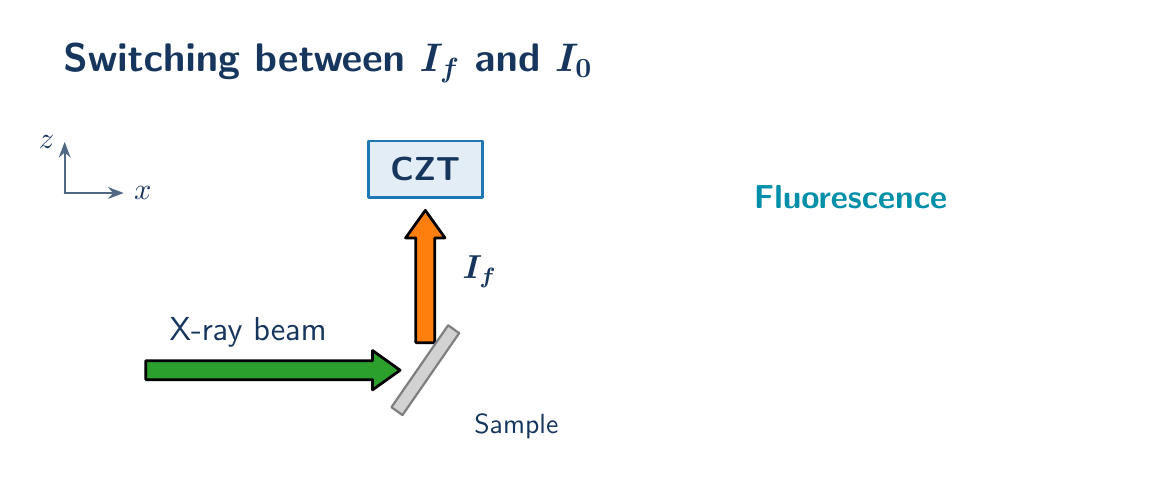
\begin{tikzpicture}[x=1cm,y=1cm,line join=round,line cap=round,
 every node/.style={font=\sffamily\fontsize{12}{14}\selectfont,text=ink},
]
\newcommand{\BeamArrow}[4]{%
  \begin{scope}
    \coordinate (beamStart) at #3;
    \coordinate (beamEnd) at #4;
    \path let \p1 = ($(beamEnd)-(beamStart)$),
      \n1 = {atan2(\y1,\x1)}, \n2 = {veclen(\x1,\y1)} in
      \pgfextra{\xdef\beamAngle{\n1}\xdef\beamLength{\n2}};
    \begin{scope}[shift={(beamStart)},rotate=\beamAngle]
      \path[fill=#1,draw=black,opacity=#2,line width=.35mm,line join=round]
        (0,-1.2mm) -- (\beamLength-3.5mm,-1.2mm)
        -- (\beamLength-3.5mm,-2.5mm) -- (\beamLength,0)
        -- (\beamLength-3.5mm,2.5mm) -- (\beamLength-3.5mm,1.2mm)
        -- (0,1.2mm) -- cycle;
    \end{scope}
  \end{scope}
}
\path[use as bounding box] (-1.05,-1.25) rectangle (12.8878,4.35);
\node[anchor=west,font=\sffamily\bfseries\fontsize{14}{17}\selectfont] at (-.72,3.9) {Switching between $\bm{I_f}$ and $\bm{I_0}$};
\draw[ink!75,line width=.8pt,-{Stealth[length=2mm]}] (-.58,2.25) -- (.17,2.25) node[anchor=west,font=\sffamily\fontsize{11}{13}\selectfont] {$x$};
\draw[ink!75,line width=.8pt,-{Stealth[length=2mm]}] (-.58,2.25) -- (-.58,2.9) node[anchor=east,font=\sffamily\fontsize{11}{13}\selectfont] {$z$};
\BeamArrow{beamgreen}{1.0000}{(.45,0)}{(3.68,0)}
\node at (1.75,.48) {X-ray beam};
\BeamArrow{beamgreen}{0.0000}{(.45,0)}{(5.98,0)}
\BeamArrow{fluororange}{1.0000}{(4,.35)}{(4,2.03)}
\node[opacity=1.0000,anchor=west] at (4.35,1.25) {$\bm{I_f}$};
\node[opacity=0.0000] at (5.25,.48) {$\bm{I_0}$};
\begin{scope}[shift={(4,0.0000)}]
\path[draw=samplegray,fill=samplegray!35,line width=.8pt] (-.43,-.47) -- (-.29,-.57) -- (.43,.47) -- (.29,.57) -- cycle;
\end{scope}
\node[anchor=west,font=\sffamily\fontsize{10}{12}\selectfont] at (4.5,-0.7200) {Sample};
\begin{scope}[shift={(4.0000,2.5500)},rotate=-0.0000,transform shape]
\node[draw=detectorblue,fill=detectorblue!13,line width=1pt,minimum width=1.45cm,minimum height=.72cm,inner sep=2pt,font=\sffamily\bfseries\fontsize{13}{15}\selectfont] {CZT};
\end{scope}
\node[opacity=1.0000,font=\sffamily\bfseries\fontsize{13}{15}\selectfont,text=motioncyan] at (9.4,2.2) {Fluorescence};
\node[opacity=0.0000,font=\sffamily\bfseries\fontsize{13}{15}\selectfont,text=motioncyan] at (9.4,2.2) {Incident beam};
\end{tikzpicture}
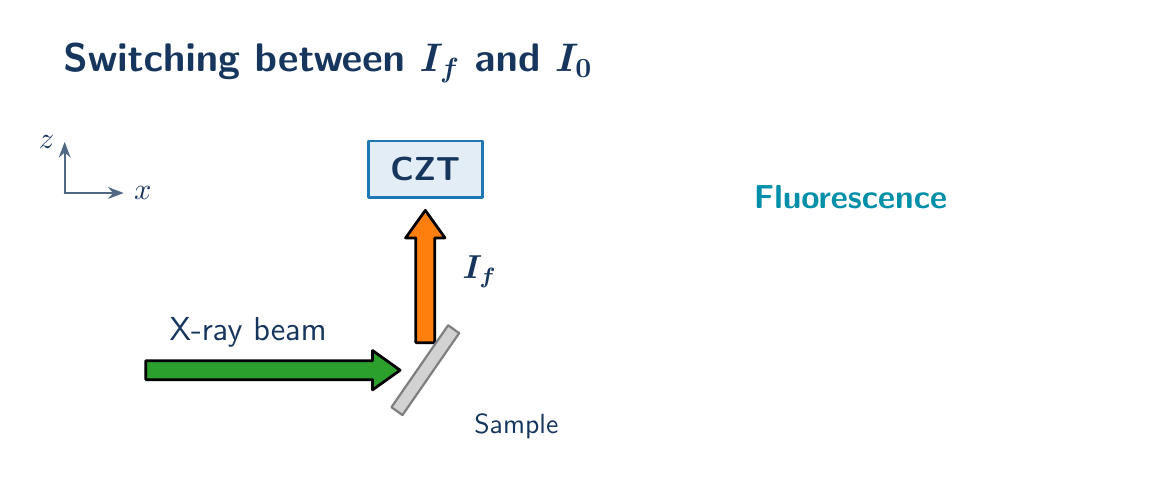
\begin{tikzpicture}[x=1cm,y=1cm,line join=round,line cap=round,
 every node/.style={font=\sffamily\fontsize{12}{14}\selectfont,text=ink},
]
\newcommand{\BeamArrow}[4]{%
  \begin{scope}
    \coordinate (beamStart) at #3;
    \coordinate (beamEnd) at #4;
    \path let \p1 = ($(beamEnd)-(beamStart)$),
      \n1 = {atan2(\y1,\x1)}, \n2 = {veclen(\x1,\y1)} in
      \pgfextra{\xdef\beamAngle{\n1}\xdef\beamLength{\n2}};
    \begin{scope}[shift={(beamStart)},rotate=\beamAngle]
      \path[fill=#1,draw=black,opacity=#2,line width=.35mm,line join=round]
        (0,-1.2mm) -- (\beamLength-3.5mm,-1.2mm)
        -- (\beamLength-3.5mm,-2.5mm) -- (\beamLength,0)
        -- (\beamLength-3.5mm,2.5mm) -- (\beamLength-3.5mm,1.2mm)
        -- (0,1.2mm) -- cycle;
    \end{scope}
  \end{scope}
}
\path[use as bounding box] (-1.05,-1.25) rectangle (12.8878,4.35);
\node[anchor=west,font=\sffamily\bfseries\fontsize{14}{17}\selectfont] at (-.72,3.9) {Switching between $\bm{I_f}$ and $\bm{I_0}$};
\draw[ink!75,line width=.8pt,-{Stealth[length=2mm]}] (-.58,2.25) -- (.17,2.25) node[anchor=west,font=\sffamily\fontsize{11}{13}\selectfont] {$x$};
\draw[ink!75,line width=.8pt,-{Stealth[length=2mm]}] (-.58,2.25) -- (-.58,2.9) node[anchor=east,font=\sffamily\fontsize{11}{13}\selectfont] {$z$};
\BeamArrow{beamgreen}{1.0000}{(.45,0)}{(3.68,0)}
\node at (1.75,.48) {X-ray beam};
\BeamArrow{beamgreen}{0.0000}{(.45,0)}{(5.98,0)}
\BeamArrow{fluororange}{1.0000}{(4,.35)}{(4,2.03)}
\node[opacity=1.0000,anchor=west] at (4.35,1.25) {$\bm{I_f}$};
\node[opacity=0.0000] at (5.25,.48) {$\bm{I_0}$};
\begin{scope}[shift={(4,0.0000)}]
\path[draw=samplegray,fill=samplegray!35,line width=.8pt] (-.43,-.47) -- (-.29,-.57) -- (.43,.47) -- (.29,.57) -- cycle;
\end{scope}
\node[anchor=west,font=\sffamily\fontsize{10}{12}\selectfont] at (4.5,-0.7200) {Sample};
\begin{scope}[shift={(4.0000,2.5500)},rotate=-0.0000,transform shape]
\node[draw=detectorblue,fill=detectorblue!13,line width=1pt,minimum width=1.45cm,minimum height=.72cm,inner sep=2pt,font=\sffamily\bfseries\fontsize{13}{15}\selectfont] {CZT};
\end{scope}
\node[opacity=1.0000,font=\sffamily\bfseries\fontsize{13}{15}\selectfont,text=motioncyan] at (9.4,2.2) {Fluorescence};
\node[opacity=0.0000,font=\sffamily\bfseries\fontsize{13}{15}\selectfont,text=motioncyan] at (9.4,2.2) {Incident beam};
\end{tikzpicture}
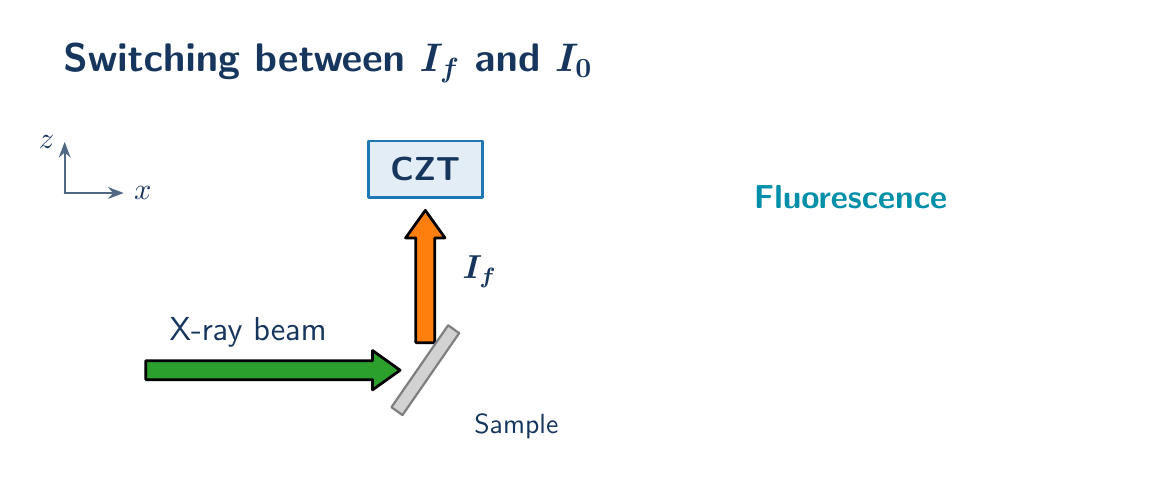
\begin{tikzpicture}[x=1cm,y=1cm,line join=round,line cap=round,
 every node/.style={font=\sffamily\fontsize{12}{14}\selectfont,text=ink},
]
\newcommand{\BeamArrow}[4]{%
  \begin{scope}
    \coordinate (beamStart) at #3;
    \coordinate (beamEnd) at #4;
    \path let \p1 = ($(beamEnd)-(beamStart)$),
      \n1 = {atan2(\y1,\x1)}, \n2 = {veclen(\x1,\y1)} in
      \pgfextra{\xdef\beamAngle{\n1}\xdef\beamLength{\n2}};
    \begin{scope}[shift={(beamStart)},rotate=\beamAngle]
      \path[fill=#1,draw=black,opacity=#2,line width=.35mm,line join=round]
        (0,-1.2mm) -- (\beamLength-3.5mm,-1.2mm)
        -- (\beamLength-3.5mm,-2.5mm) -- (\beamLength,0)
        -- (\beamLength-3.5mm,2.5mm) -- (\beamLength-3.5mm,1.2mm)
        -- (0,1.2mm) -- cycle;
    \end{scope}
  \end{scope}
}
\path[use as bounding box] (-1.05,-1.25) rectangle (12.8878,4.35);
\node[anchor=west,font=\sffamily\bfseries\fontsize{14}{17}\selectfont] at (-.72,3.9) {Switching between $\bm{I_f}$ and $\bm{I_0}$};
\draw[ink!75,line width=.8pt,-{Stealth[length=2mm]}] (-.58,2.25) -- (.17,2.25) node[anchor=west,font=\sffamily\fontsize{11}{13}\selectfont] {$x$};
\draw[ink!75,line width=.8pt,-{Stealth[length=2mm]}] (-.58,2.25) -- (-.58,2.9) node[anchor=east,font=\sffamily\fontsize{11}{13}\selectfont] {$z$};
\BeamArrow{beamgreen}{1.0000}{(.45,0)}{(3.68,0)}
\node at (1.75,.48) {X-ray beam};
\BeamArrow{beamgreen}{0.0000}{(.45,0)}{(5.98,0)}
\BeamArrow{fluororange}{1.0000}{(4,.35)}{(4,2.03)}
\node[opacity=1.0000,anchor=west] at (4.35,1.25) {$\bm{I_f}$};
\node[opacity=0.0000] at (5.25,.48) {$\bm{I_0}$};
\begin{scope}[shift={(4,0.0000)}]
\path[draw=samplegray,fill=samplegray!35,line width=.8pt] (-.43,-.47) -- (-.29,-.57) -- (.43,.47) -- (.29,.57) -- cycle;
\end{scope}
\node[anchor=west,font=\sffamily\fontsize{10}{12}\selectfont] at (4.5,-0.7200) {Sample};
\begin{scope}[shift={(4.0000,2.5500)},rotate=-0.0000,transform shape]
\node[draw=detectorblue,fill=detectorblue!13,line width=1pt,minimum width=1.45cm,minimum height=.72cm,inner sep=2pt,font=\sffamily\bfseries\fontsize{13}{15}\selectfont] {CZT};
\end{scope}
\node[opacity=1.0000,font=\sffamily\bfseries\fontsize{13}{15}\selectfont,text=motioncyan] at (9.4,2.2) {Fluorescence};
\node[opacity=0.0000,font=\sffamily\bfseries\fontsize{13}{15}\selectfont,text=motioncyan] at (9.4,2.2) {Incident beam};
\end{tikzpicture}
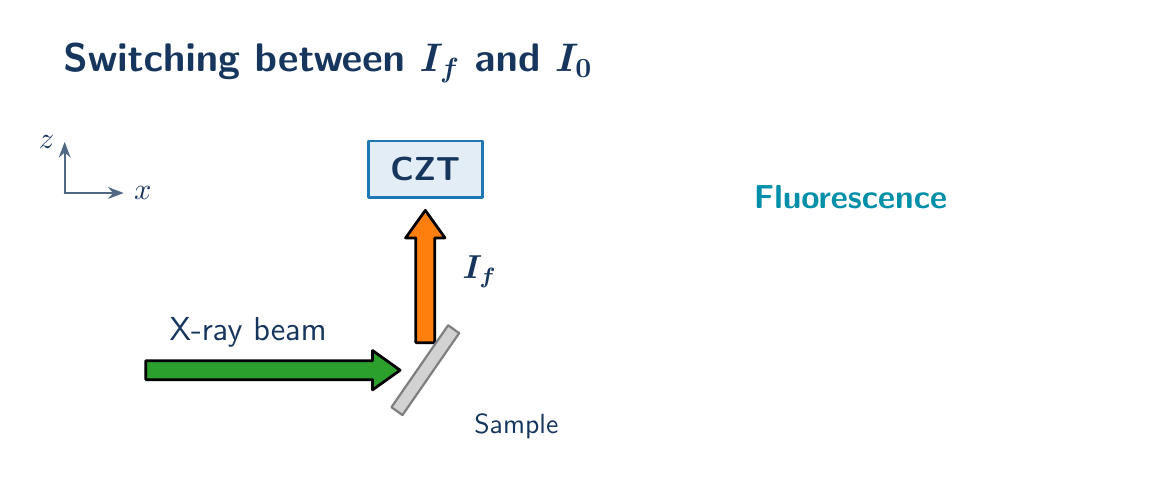
\begin{tikzpicture}[x=1cm,y=1cm,line join=round,line cap=round,
 every node/.style={font=\sffamily\fontsize{12}{14}\selectfont,text=ink},
]
\newcommand{\BeamArrow}[4]{%
  \begin{scope}
    \coordinate (beamStart) at #3;
    \coordinate (beamEnd) at #4;
    \path let \p1 = ($(beamEnd)-(beamStart)$),
      \n1 = {atan2(\y1,\x1)}, \n2 = {veclen(\x1,\y1)} in
      \pgfextra{\xdef\beamAngle{\n1}\xdef\beamLength{\n2}};
    \begin{scope}[shift={(beamStart)},rotate=\beamAngle]
      \path[fill=#1,draw=black,opacity=#2,line width=.35mm,line join=round]
        (0,-1.2mm) -- (\beamLength-3.5mm,-1.2mm)
        -- (\beamLength-3.5mm,-2.5mm) -- (\beamLength,0)
        -- (\beamLength-3.5mm,2.5mm) -- (\beamLength-3.5mm,1.2mm)
        -- (0,1.2mm) -- cycle;
    \end{scope}
  \end{scope}
}
\path[use as bounding box] (-1.05,-1.25) rectangle (12.8878,4.35);
\node[anchor=west,font=\sffamily\bfseries\fontsize{14}{17}\selectfont] at (-.72,3.9) {Switching between $\bm{I_f}$ and $\bm{I_0}$};
\draw[ink!75,line width=.8pt,-{Stealth[length=2mm]}] (-.58,2.25) -- (.17,2.25) node[anchor=west,font=\sffamily\fontsize{11}{13}\selectfont] {$x$};
\draw[ink!75,line width=.8pt,-{Stealth[length=2mm]}] (-.58,2.25) -- (-.58,2.9) node[anchor=east,font=\sffamily\fontsize{11}{13}\selectfont] {$z$};
\BeamArrow{beamgreen}{1.0000}{(.45,0)}{(3.68,0)}
\node at (1.75,.48) {X-ray beam};
\BeamArrow{beamgreen}{0.0000}{(.45,0)}{(5.98,0)}
\BeamArrow{fluororange}{1.0000}{(4,.35)}{(4,2.03)}
\node[opacity=1.0000,anchor=west] at (4.35,1.25) {$\bm{I_f}$};
\node[opacity=0.0000] at (5.25,.48) {$\bm{I_0}$};
\begin{scope}[shift={(4,0.0000)}]
\path[draw=samplegray,fill=samplegray!35,line width=.8pt] (-.43,-.47) -- (-.29,-.57) -- (.43,.47) -- (.29,.57) -- cycle;
\end{scope}
\node[anchor=west,font=\sffamily\fontsize{10}{12}\selectfont] at (4.5,-0.7200) {Sample};
\begin{scope}[shift={(4.0000,2.5500)},rotate=-0.0000,transform shape]
\node[draw=detectorblue,fill=detectorblue!13,line width=1pt,minimum width=1.45cm,minimum height=.72cm,inner sep=2pt,font=\sffamily\bfseries\fontsize{13}{15}\selectfont] {CZT};
\end{scope}
\node[opacity=1.0000,font=\sffamily\bfseries\fontsize{13}{15}\selectfont,text=motioncyan] at (9.4,2.2) {Fluorescence};
\node[opacity=0.0000,font=\sffamily\bfseries\fontsize{13}{15}\selectfont,text=motioncyan] at (9.4,2.2) {Incident beam};
\end{tikzpicture}
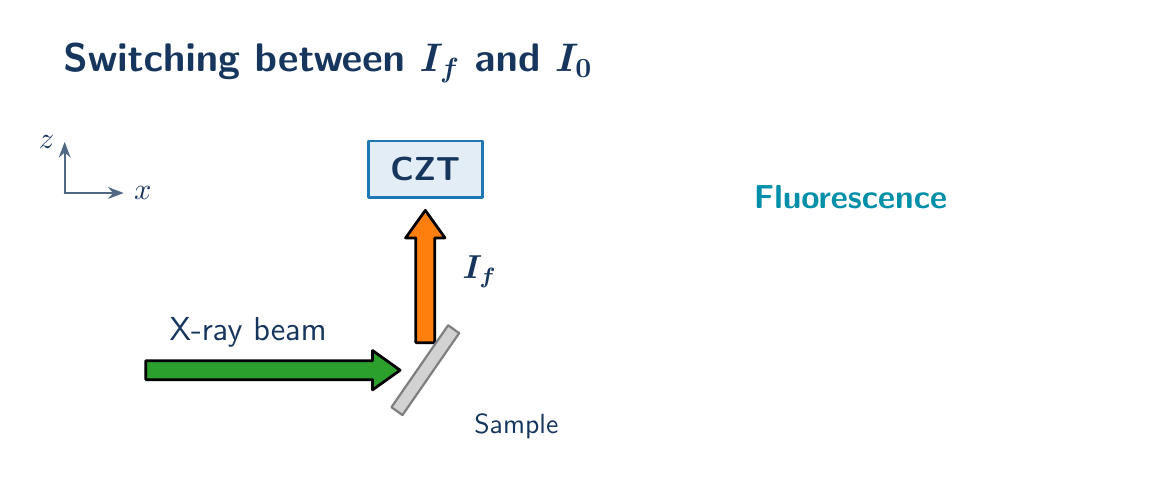
\begin{tikzpicture}[x=1cm,y=1cm,line join=round,line cap=round,
 every node/.style={font=\sffamily\fontsize{12}{14}\selectfont,text=ink},
]
\newcommand{\BeamArrow}[4]{%
  \begin{scope}
    \coordinate (beamStart) at #3;
    \coordinate (beamEnd) at #4;
    \path let \p1 = ($(beamEnd)-(beamStart)$),
      \n1 = {atan2(\y1,\x1)}, \n2 = {veclen(\x1,\y1)} in
      \pgfextra{\xdef\beamAngle{\n1}\xdef\beamLength{\n2}};
    \begin{scope}[shift={(beamStart)},rotate=\beamAngle]
      \path[fill=#1,draw=black,opacity=#2,line width=.35mm,line join=round]
        (0,-1.2mm) -- (\beamLength-3.5mm,-1.2mm)
        -- (\beamLength-3.5mm,-2.5mm) -- (\beamLength,0)
        -- (\beamLength-3.5mm,2.5mm) -- (\beamLength-3.5mm,1.2mm)
        -- (0,1.2mm) -- cycle;
    \end{scope}
  \end{scope}
}
\path[use as bounding box] (-1.05,-1.25) rectangle (12.8878,4.35);
\node[anchor=west,font=\sffamily\bfseries\fontsize{14}{17}\selectfont] at (-.72,3.9) {Switching between $\bm{I_f}$ and $\bm{I_0}$};
\draw[ink!75,line width=.8pt,-{Stealth[length=2mm]}] (-.58,2.25) -- (.17,2.25) node[anchor=west,font=\sffamily\fontsize{11}{13}\selectfont] {$x$};
\draw[ink!75,line width=.8pt,-{Stealth[length=2mm]}] (-.58,2.25) -- (-.58,2.9) node[anchor=east,font=\sffamily\fontsize{11}{13}\selectfont] {$z$};
\BeamArrow{beamgreen}{1.0000}{(.45,0)}{(3.68,0)}
\node at (1.75,.48) {X-ray beam};
\BeamArrow{beamgreen}{0.0000}{(.45,0)}{(5.98,0)}
\BeamArrow{fluororange}{1.0000}{(4,.35)}{(4,2.03)}
\node[opacity=1.0000,anchor=west] at (4.35,1.25) {$\bm{I_f}$};
\node[opacity=0.0000] at (5.25,.48) {$\bm{I_0}$};
\begin{scope}[shift={(4,0.0000)}]
\path[draw=samplegray,fill=samplegray!35,line width=.8pt] (-.43,-.47) -- (-.29,-.57) -- (.43,.47) -- (.29,.57) -- cycle;
\end{scope}
\node[anchor=west,font=\sffamily\fontsize{10}{12}\selectfont] at (4.5,-0.7200) {Sample};
\begin{scope}[shift={(4.0000,2.5500)},rotate=-0.0000,transform shape]
\node[draw=detectorblue,fill=detectorblue!13,line width=1pt,minimum width=1.45cm,minimum height=.72cm,inner sep=2pt,font=\sffamily\bfseries\fontsize{13}{15}\selectfont] {CZT};
\end{scope}
\node[opacity=1.0000,font=\sffamily\bfseries\fontsize{13}{15}\selectfont,text=motioncyan] at (9.4,2.2) {Fluorescence};
\node[opacity=0.0000,font=\sffamily\bfseries\fontsize{13}{15}\selectfont,text=motioncyan] at (9.4,2.2) {Incident beam};
\end{tikzpicture}
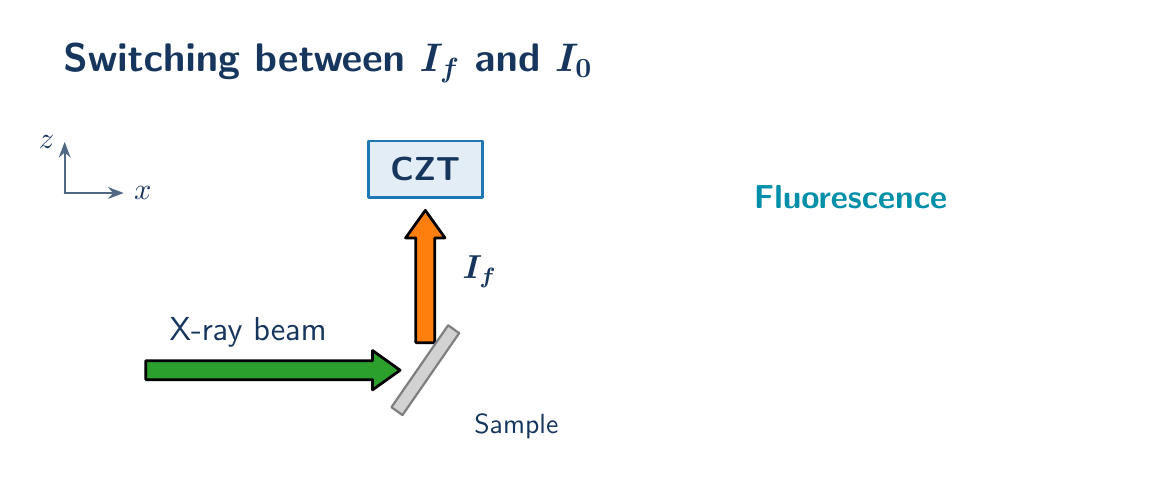
\begin{tikzpicture}[x=1cm,y=1cm,line join=round,line cap=round,
 every node/.style={font=\sffamily\fontsize{12}{14}\selectfont,text=ink},
]
\newcommand{\BeamArrow}[4]{%
  \begin{scope}
    \coordinate (beamStart) at #3;
    \coordinate (beamEnd) at #4;
    \path let \p1 = ($(beamEnd)-(beamStart)$),
      \n1 = {atan2(\y1,\x1)}, \n2 = {veclen(\x1,\y1)} in
      \pgfextra{\xdef\beamAngle{\n1}\xdef\beamLength{\n2}};
    \begin{scope}[shift={(beamStart)},rotate=\beamAngle]
      \path[fill=#1,draw=black,opacity=#2,line width=.35mm,line join=round]
        (0,-1.2mm) -- (\beamLength-3.5mm,-1.2mm)
        -- (\beamLength-3.5mm,-2.5mm) -- (\beamLength,0)
        -- (\beamLength-3.5mm,2.5mm) -- (\beamLength-3.5mm,1.2mm)
        -- (0,1.2mm) -- cycle;
    \end{scope}
  \end{scope}
}
\path[use as bounding box] (-1.05,-1.25) rectangle (12.8878,4.35);
\node[anchor=west,font=\sffamily\bfseries\fontsize{14}{17}\selectfont] at (-.72,3.9) {Switching between $\bm{I_f}$ and $\bm{I_0}$};
\draw[ink!75,line width=.8pt,-{Stealth[length=2mm]}] (-.58,2.25) -- (.17,2.25) node[anchor=west,font=\sffamily\fontsize{11}{13}\selectfont] {$x$};
\draw[ink!75,line width=.8pt,-{Stealth[length=2mm]}] (-.58,2.25) -- (-.58,2.9) node[anchor=east,font=\sffamily\fontsize{11}{13}\selectfont] {$z$};
\BeamArrow{beamgreen}{1.0000}{(.45,0)}{(3.68,0)}
\node at (1.75,.48) {X-ray beam};
\BeamArrow{beamgreen}{0.0000}{(.45,0)}{(5.98,0)}
\BeamArrow{fluororange}{1.0000}{(4,.35)}{(4,2.03)}
\node[opacity=1.0000,anchor=west] at (4.35,1.25) {$\bm{I_f}$};
\node[opacity=0.0000] at (5.25,.48) {$\bm{I_0}$};
\begin{scope}[shift={(4,0.0000)}]
\path[draw=samplegray,fill=samplegray!35,line width=.8pt] (-.43,-.47) -- (-.29,-.57) -- (.43,.47) -- (.29,.57) -- cycle;
\end{scope}
\node[anchor=west,font=\sffamily\fontsize{10}{12}\selectfont] at (4.5,-0.7200) {Sample};
\begin{scope}[shift={(4.0000,2.5500)},rotate=-0.0000,transform shape]
\node[draw=detectorblue,fill=detectorblue!13,line width=1pt,minimum width=1.45cm,minimum height=.72cm,inner sep=2pt,font=\sffamily\bfseries\fontsize{13}{15}\selectfont] {CZT};
\end{scope}
\node[opacity=1.0000,font=\sffamily\bfseries\fontsize{13}{15}\selectfont,text=motioncyan] at (9.4,2.2) {Fluorescence};
\node[opacity=0.0000,font=\sffamily\bfseries\fontsize{13}{15}\selectfont,text=motioncyan] at (9.4,2.2) {Incident beam};
\end{tikzpicture}
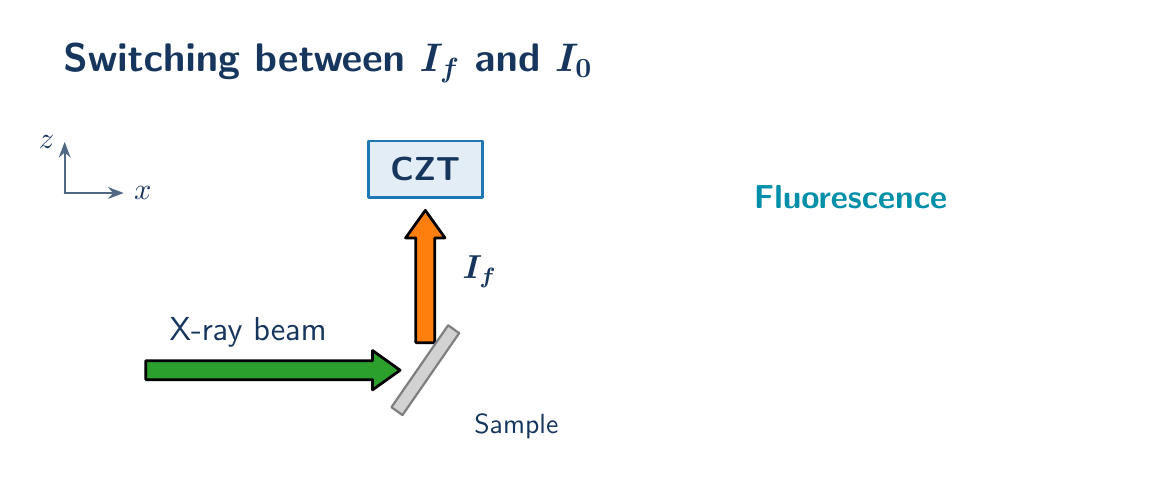
\begin{tikzpicture}[x=1cm,y=1cm,line join=round,line cap=round,
 every node/.style={font=\sffamily\fontsize{12}{14}\selectfont,text=ink},
]
\newcommand{\BeamArrow}[4]{%
  \begin{scope}
    \coordinate (beamStart) at #3;
    \coordinate (beamEnd) at #4;
    \path let \p1 = ($(beamEnd)-(beamStart)$),
      \n1 = {atan2(\y1,\x1)}, \n2 = {veclen(\x1,\y1)} in
      \pgfextra{\xdef\beamAngle{\n1}\xdef\beamLength{\n2}};
    \begin{scope}[shift={(beamStart)},rotate=\beamAngle]
      \path[fill=#1,draw=black,opacity=#2,line width=.35mm,line join=round]
        (0,-1.2mm) -- (\beamLength-3.5mm,-1.2mm)
        -- (\beamLength-3.5mm,-2.5mm) -- (\beamLength,0)
        -- (\beamLength-3.5mm,2.5mm) -- (\beamLength-3.5mm,1.2mm)
        -- (0,1.2mm) -- cycle;
    \end{scope}
  \end{scope}
}
\path[use as bounding box] (-1.05,-1.25) rectangle (12.8878,4.35);
\node[anchor=west,font=\sffamily\bfseries\fontsize{14}{17}\selectfont] at (-.72,3.9) {Switching between $\bm{I_f}$ and $\bm{I_0}$};
\draw[ink!75,line width=.8pt,-{Stealth[length=2mm]}] (-.58,2.25) -- (.17,2.25) node[anchor=west,font=\sffamily\fontsize{11}{13}\selectfont] {$x$};
\draw[ink!75,line width=.8pt,-{Stealth[length=2mm]}] (-.58,2.25) -- (-.58,2.9) node[anchor=east,font=\sffamily\fontsize{11}{13}\selectfont] {$z$};
\BeamArrow{beamgreen}{1.0000}{(.45,0)}{(3.68,0)}
\node at (1.75,.48) {X-ray beam};
\BeamArrow{beamgreen}{0.0000}{(.45,0)}{(5.98,0)}
\BeamArrow{fluororange}{1.0000}{(4,.35)}{(4,2.03)}
\node[opacity=1.0000,anchor=west] at (4.35,1.25) {$\bm{I_f}$};
\node[opacity=0.0000] at (5.25,.48) {$\bm{I_0}$};
\begin{scope}[shift={(4,0.0000)}]
\path[draw=samplegray,fill=samplegray!35,line width=.8pt] (-.43,-.47) -- (-.29,-.57) -- (.43,.47) -- (.29,.57) -- cycle;
\end{scope}
\node[anchor=west,font=\sffamily\fontsize{10}{12}\selectfont] at (4.5,-0.7200) {Sample};
\begin{scope}[shift={(4.0000,2.5500)},rotate=-0.0000,transform shape]
\node[draw=detectorblue,fill=detectorblue!13,line width=1pt,minimum width=1.45cm,minimum height=.72cm,inner sep=2pt,font=\sffamily\bfseries\fontsize{13}{15}\selectfont] {CZT};
\end{scope}
\node[opacity=1.0000,font=\sffamily\bfseries\fontsize{13}{15}\selectfont,text=motioncyan] at (9.4,2.2) {Fluorescence};
\node[opacity=0.0000,font=\sffamily\bfseries\fontsize{13}{15}\selectfont,text=motioncyan] at (9.4,2.2) {Incident beam};
\end{tikzpicture}
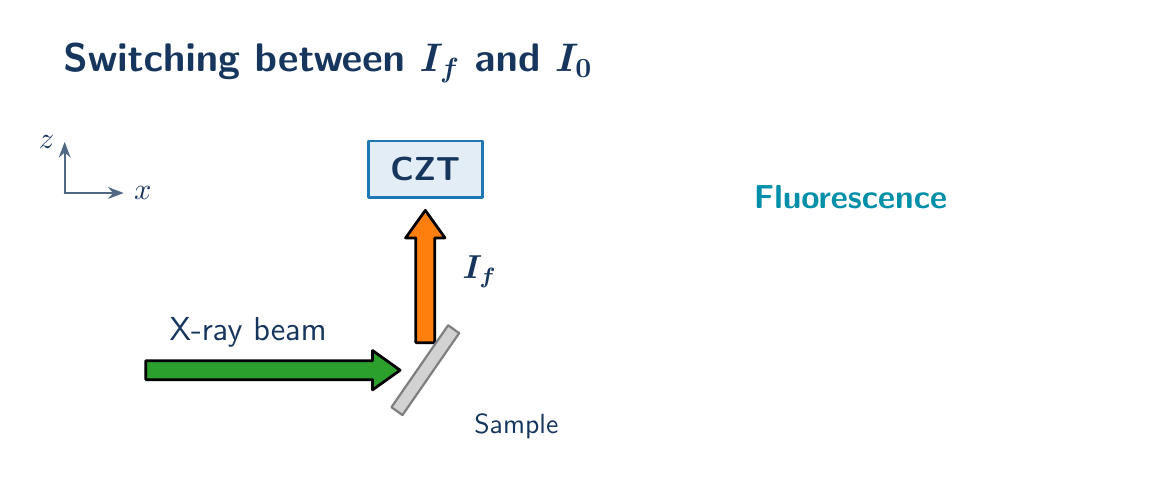
\begin{tikzpicture}[x=1cm,y=1cm,line join=round,line cap=round,
 every node/.style={font=\sffamily\fontsize{12}{14}\selectfont,text=ink},
]
\newcommand{\BeamArrow}[4]{%
  \begin{scope}
    \coordinate (beamStart) at #3;
    \coordinate (beamEnd) at #4;
    \path let \p1 = ($(beamEnd)-(beamStart)$),
      \n1 = {atan2(\y1,\x1)}, \n2 = {veclen(\x1,\y1)} in
      \pgfextra{\xdef\beamAngle{\n1}\xdef\beamLength{\n2}};
    \begin{scope}[shift={(beamStart)},rotate=\beamAngle]
      \path[fill=#1,draw=black,opacity=#2,line width=.35mm,line join=round]
        (0,-1.2mm) -- (\beamLength-3.5mm,-1.2mm)
        -- (\beamLength-3.5mm,-2.5mm) -- (\beamLength,0)
        -- (\beamLength-3.5mm,2.5mm) -- (\beamLength-3.5mm,1.2mm)
        -- (0,1.2mm) -- cycle;
    \end{scope}
  \end{scope}
}
\path[use as bounding box] (-1.05,-1.25) rectangle (12.8878,4.35);
\node[anchor=west,font=\sffamily\bfseries\fontsize{14}{17}\selectfont] at (-.72,3.9) {Switching between $\bm{I_f}$ and $\bm{I_0}$};
\draw[ink!75,line width=.8pt,-{Stealth[length=2mm]}] (-.58,2.25) -- (.17,2.25) node[anchor=west,font=\sffamily\fontsize{11}{13}\selectfont] {$x$};
\draw[ink!75,line width=.8pt,-{Stealth[length=2mm]}] (-.58,2.25) -- (-.58,2.9) node[anchor=east,font=\sffamily\fontsize{11}{13}\selectfont] {$z$};
\BeamArrow{beamgreen}{1.0000}{(.45,0)}{(3.68,0)}
\node at (1.75,.48) {X-ray beam};
\BeamArrow{beamgreen}{0.0000}{(.45,0)}{(5.98,0)}
\BeamArrow{fluororange}{1.0000}{(4,.35)}{(4,2.03)}
\node[opacity=1.0000,anchor=west] at (4.35,1.25) {$\bm{I_f}$};
\node[opacity=0.0000] at (5.25,.48) {$\bm{I_0}$};
\begin{scope}[shift={(4,0.0000)}]
\path[draw=samplegray,fill=samplegray!35,line width=.8pt] (-.43,-.47) -- (-.29,-.57) -- (.43,.47) -- (.29,.57) -- cycle;
\end{scope}
\node[anchor=west,font=\sffamily\fontsize{10}{12}\selectfont] at (4.5,-0.7200) {Sample};
\begin{scope}[shift={(4.0000,2.5500)},rotate=-0.0000,transform shape]
\node[draw=detectorblue,fill=detectorblue!13,line width=1pt,minimum width=1.45cm,minimum height=.72cm,inner sep=2pt,font=\sffamily\bfseries\fontsize{13}{15}\selectfont] {CZT};
\end{scope}
\node[opacity=1.0000,font=\sffamily\bfseries\fontsize{13}{15}\selectfont,text=motioncyan] at (9.4,2.2) {Fluorescence};
\node[opacity=0.0000,font=\sffamily\bfseries\fontsize{13}{15}\selectfont,text=motioncyan] at (9.4,2.2) {Incident beam};
\end{tikzpicture}
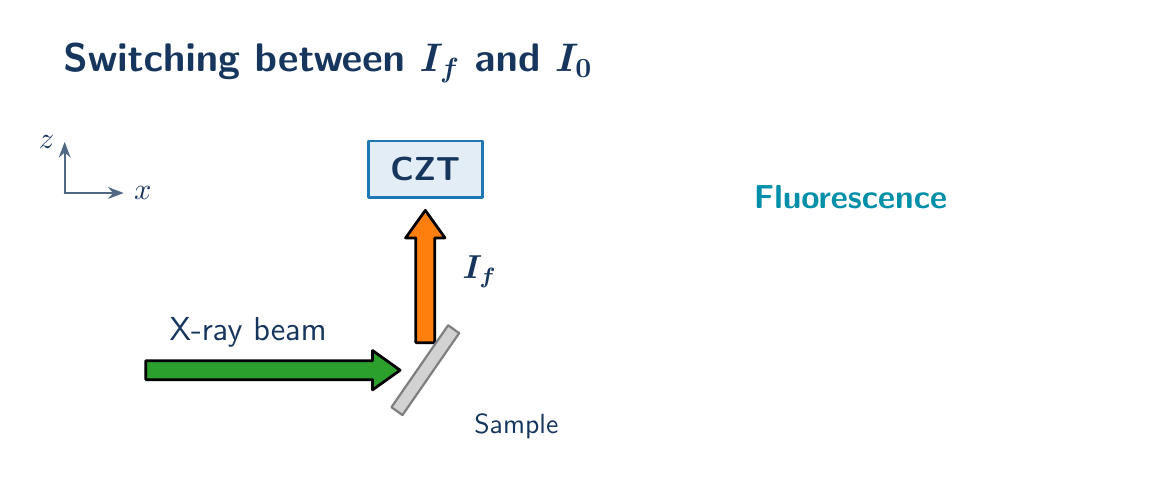
\begin{tikzpicture}[x=1cm,y=1cm,line join=round,line cap=round,
 every node/.style={font=\sffamily\fontsize{12}{14}\selectfont,text=ink},
]
\newcommand{\BeamArrow}[4]{%
  \begin{scope}
    \coordinate (beamStart) at #3;
    \coordinate (beamEnd) at #4;
    \path let \p1 = ($(beamEnd)-(beamStart)$),
      \n1 = {atan2(\y1,\x1)}, \n2 = {veclen(\x1,\y1)} in
      \pgfextra{\xdef\beamAngle{\n1}\xdef\beamLength{\n2}};
    \begin{scope}[shift={(beamStart)},rotate=\beamAngle]
      \path[fill=#1,draw=black,opacity=#2,line width=.35mm,line join=round]
        (0,-1.2mm) -- (\beamLength-3.5mm,-1.2mm)
        -- (\beamLength-3.5mm,-2.5mm) -- (\beamLength,0)
        -- (\beamLength-3.5mm,2.5mm) -- (\beamLength-3.5mm,1.2mm)
        -- (0,1.2mm) -- cycle;
    \end{scope}
  \end{scope}
}
\path[use as bounding box] (-1.05,-1.25) rectangle (12.8878,4.35);
\node[anchor=west,font=\sffamily\bfseries\fontsize{14}{17}\selectfont] at (-.72,3.9) {Switching between $\bm{I_f}$ and $\bm{I_0}$};
\draw[ink!75,line width=.8pt,-{Stealth[length=2mm]}] (-.58,2.25) -- (.17,2.25) node[anchor=west,font=\sffamily\fontsize{11}{13}\selectfont] {$x$};
\draw[ink!75,line width=.8pt,-{Stealth[length=2mm]}] (-.58,2.25) -- (-.58,2.9) node[anchor=east,font=\sffamily\fontsize{11}{13}\selectfont] {$z$};
\BeamArrow{beamgreen}{1.0000}{(.45,0)}{(3.68,0)}
\node at (1.75,.48) {X-ray beam};
\BeamArrow{beamgreen}{0.0000}{(.45,0)}{(5.98,0)}
\BeamArrow{fluororange}{1.0000}{(4,.35)}{(4,2.03)}
\node[opacity=1.0000,anchor=west] at (4.35,1.25) {$\bm{I_f}$};
\node[opacity=0.0000] at (5.25,.48) {$\bm{I_0}$};
\begin{scope}[shift={(4,0.0000)}]
\path[draw=samplegray,fill=samplegray!35,line width=.8pt] (-.43,-.47) -- (-.29,-.57) -- (.43,.47) -- (.29,.57) -- cycle;
\end{scope}
\node[anchor=west,font=\sffamily\fontsize{10}{12}\selectfont] at (4.5,-0.7200) {Sample};
\begin{scope}[shift={(4.0000,2.5500)},rotate=-0.0000,transform shape]
\node[draw=detectorblue,fill=detectorblue!13,line width=1pt,minimum width=1.45cm,minimum height=.72cm,inner sep=2pt,font=\sffamily\bfseries\fontsize{13}{15}\selectfont] {CZT};
\end{scope}
\node[opacity=1.0000,font=\sffamily\bfseries\fontsize{13}{15}\selectfont,text=motioncyan] at (9.4,2.2) {Fluorescence};
\node[opacity=0.0000,font=\sffamily\bfseries\fontsize{13}{15}\selectfont,text=motioncyan] at (9.4,2.2) {Incident beam};
\end{tikzpicture}
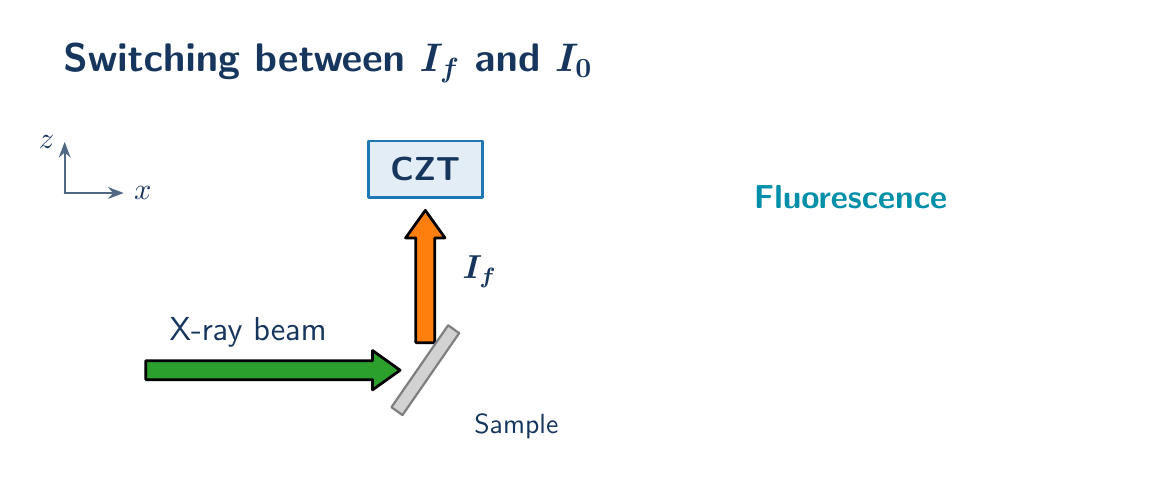
\begin{tikzpicture}[x=1cm,y=1cm,line join=round,line cap=round,
 every node/.style={font=\sffamily\fontsize{12}{14}\selectfont,text=ink},
]
\newcommand{\BeamArrow}[4]{%
  \begin{scope}
    \coordinate (beamStart) at #3;
    \coordinate (beamEnd) at #4;
    \path let \p1 = ($(beamEnd)-(beamStart)$),
      \n1 = {atan2(\y1,\x1)}, \n2 = {veclen(\x1,\y1)} in
      \pgfextra{\xdef\beamAngle{\n1}\xdef\beamLength{\n2}};
    \begin{scope}[shift={(beamStart)},rotate=\beamAngle]
      \path[fill=#1,draw=black,opacity=#2,line width=.35mm,line join=round]
        (0,-1.2mm) -- (\beamLength-3.5mm,-1.2mm)
        -- (\beamLength-3.5mm,-2.5mm) -- (\beamLength,0)
        -- (\beamLength-3.5mm,2.5mm) -- (\beamLength-3.5mm,1.2mm)
        -- (0,1.2mm) -- cycle;
    \end{scope}
  \end{scope}
}
\path[use as bounding box] (-1.05,-1.25) rectangle (12.8878,4.35);
\node[anchor=west,font=\sffamily\bfseries\fontsize{14}{17}\selectfont] at (-.72,3.9) {Switching between $\bm{I_f}$ and $\bm{I_0}$};
\draw[ink!75,line width=.8pt,-{Stealth[length=2mm]}] (-.58,2.25) -- (.17,2.25) node[anchor=west,font=\sffamily\fontsize{11}{13}\selectfont] {$x$};
\draw[ink!75,line width=.8pt,-{Stealth[length=2mm]}] (-.58,2.25) -- (-.58,2.9) node[anchor=east,font=\sffamily\fontsize{11}{13}\selectfont] {$z$};
\BeamArrow{beamgreen}{1.0000}{(.45,0)}{(3.68,0)}
\node at (1.75,.48) {X-ray beam};
\BeamArrow{beamgreen}{0.0000}{(.45,0)}{(5.98,0)}
\BeamArrow{fluororange}{1.0000}{(4,.35)}{(4,2.03)}
\node[opacity=1.0000,anchor=west] at (4.35,1.25) {$\bm{I_f}$};
\node[opacity=0.0000] at (5.25,.48) {$\bm{I_0}$};
\begin{scope}[shift={(4,0.0000)}]
\path[draw=samplegray,fill=samplegray!35,line width=.8pt] (-.43,-.47) -- (-.29,-.57) -- (.43,.47) -- (.29,.57) -- cycle;
\end{scope}
\node[anchor=west,font=\sffamily\fontsize{10}{12}\selectfont] at (4.5,-0.7200) {Sample};
\begin{scope}[shift={(4.0000,2.5500)},rotate=-0.0000,transform shape]
\node[draw=detectorblue,fill=detectorblue!13,line width=1pt,minimum width=1.45cm,minimum height=.72cm,inner sep=2pt,font=\sffamily\bfseries\fontsize{13}{15}\selectfont] {CZT};
\end{scope}
\node[opacity=1.0000,font=\sffamily\bfseries\fontsize{13}{15}\selectfont,text=motioncyan] at (9.4,2.2) {Fluorescence};
\node[opacity=0.0000,font=\sffamily\bfseries\fontsize{13}{15}\selectfont,text=motioncyan] at (9.4,2.2) {Incident beam};
\end{tikzpicture}
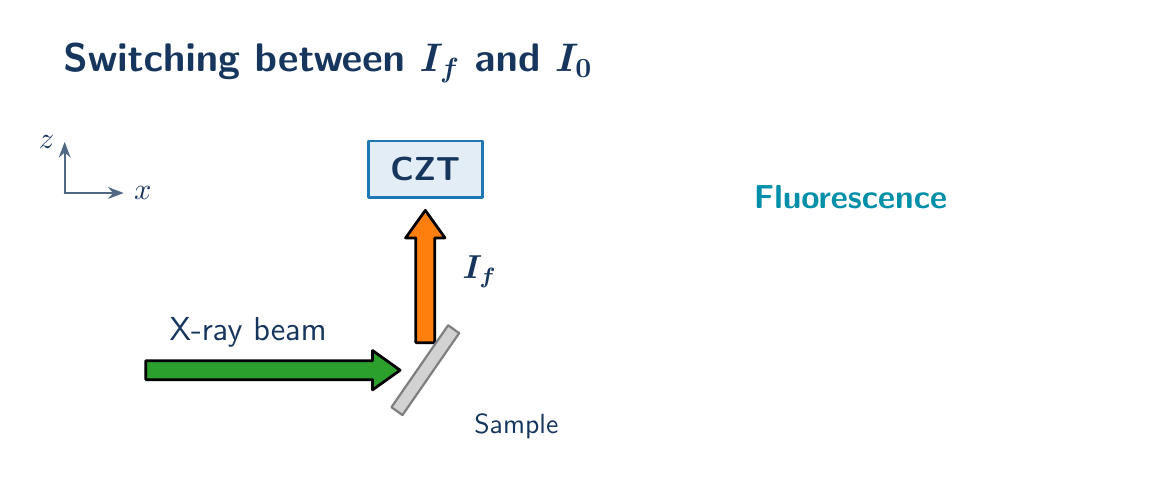
\begin{tikzpicture}[x=1cm,y=1cm,line join=round,line cap=round,
 every node/.style={font=\sffamily\fontsize{12}{14}\selectfont,text=ink},
]
\newcommand{\BeamArrow}[4]{%
  \begin{scope}
    \coordinate (beamStart) at #3;
    \coordinate (beamEnd) at #4;
    \path let \p1 = ($(beamEnd)-(beamStart)$),
      \n1 = {atan2(\y1,\x1)}, \n2 = {veclen(\x1,\y1)} in
      \pgfextra{\xdef\beamAngle{\n1}\xdef\beamLength{\n2}};
    \begin{scope}[shift={(beamStart)},rotate=\beamAngle]
      \path[fill=#1,draw=black,opacity=#2,line width=.35mm,line join=round]
        (0,-1.2mm) -- (\beamLength-3.5mm,-1.2mm)
        -- (\beamLength-3.5mm,-2.5mm) -- (\beamLength,0)
        -- (\beamLength-3.5mm,2.5mm) -- (\beamLength-3.5mm,1.2mm)
        -- (0,1.2mm) -- cycle;
    \end{scope}
  \end{scope}
}
\path[use as bounding box] (-1.05,-1.25) rectangle (12.8878,4.35);
\node[anchor=west,font=\sffamily\bfseries\fontsize{14}{17}\selectfont] at (-.72,3.9) {Switching between $\bm{I_f}$ and $\bm{I_0}$};
\draw[ink!75,line width=.8pt,-{Stealth[length=2mm]}] (-.58,2.25) -- (.17,2.25) node[anchor=west,font=\sffamily\fontsize{11}{13}\selectfont] {$x$};
\draw[ink!75,line width=.8pt,-{Stealth[length=2mm]}] (-.58,2.25) -- (-.58,2.9) node[anchor=east,font=\sffamily\fontsize{11}{13}\selectfont] {$z$};
\BeamArrow{beamgreen}{1.0000}{(.45,0)}{(3.68,0)}
\node at (1.75,.48) {X-ray beam};
\BeamArrow{beamgreen}{0.0000}{(.45,0)}{(5.98,0)}
\BeamArrow{fluororange}{1.0000}{(4,.35)}{(4,2.03)}
\node[opacity=1.0000,anchor=west] at (4.35,1.25) {$\bm{I_f}$};
\node[opacity=0.0000] at (5.25,.48) {$\bm{I_0}$};
\begin{scope}[shift={(4,0.0000)}]
\path[draw=samplegray,fill=samplegray!35,line width=.8pt] (-.43,-.47) -- (-.29,-.57) -- (.43,.47) -- (.29,.57) -- cycle;
\end{scope}
\node[anchor=west,font=\sffamily\fontsize{10}{12}\selectfont] at (4.5,-0.7200) {Sample};
\begin{scope}[shift={(4.0000,2.5500)},rotate=-0.0000,transform shape]
\node[draw=detectorblue,fill=detectorblue!13,line width=1pt,minimum width=1.45cm,minimum height=.72cm,inner sep=2pt,font=\sffamily\bfseries\fontsize{13}{15}\selectfont] {CZT};
\end{scope}
\node[opacity=1.0000,font=\sffamily\bfseries\fontsize{13}{15}\selectfont,text=motioncyan] at (9.4,2.2) {Fluorescence};
\node[opacity=0.0000,font=\sffamily\bfseries\fontsize{13}{15}\selectfont,text=motioncyan] at (9.4,2.2) {Incident beam};
\end{tikzpicture}
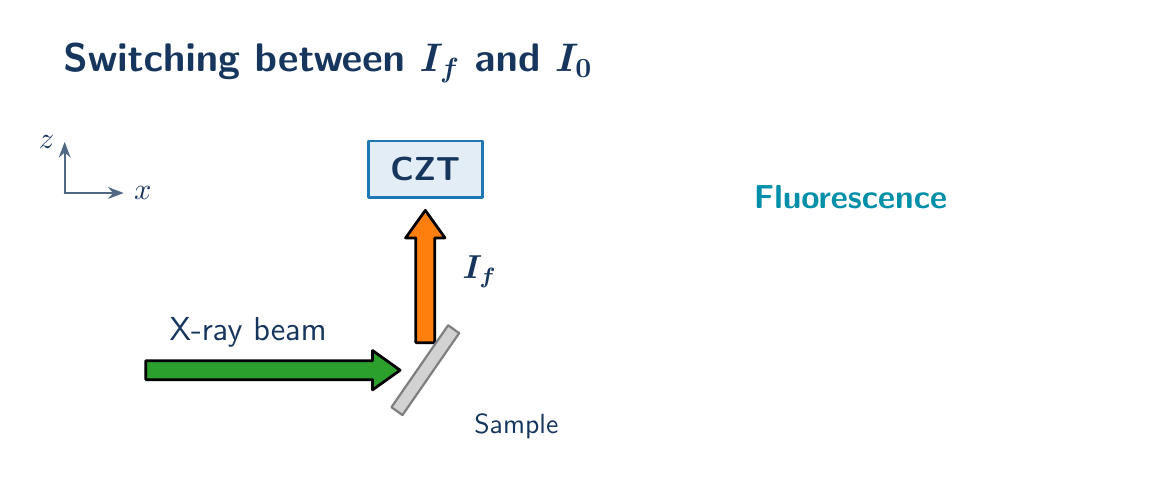
\begin{tikzpicture}[x=1cm,y=1cm,line join=round,line cap=round,
 every node/.style={font=\sffamily\fontsize{12}{14}\selectfont,text=ink},
]
\newcommand{\BeamArrow}[4]{%
  \begin{scope}
    \coordinate (beamStart) at #3;
    \coordinate (beamEnd) at #4;
    \path let \p1 = ($(beamEnd)-(beamStart)$),
      \n1 = {atan2(\y1,\x1)}, \n2 = {veclen(\x1,\y1)} in
      \pgfextra{\xdef\beamAngle{\n1}\xdef\beamLength{\n2}};
    \begin{scope}[shift={(beamStart)},rotate=\beamAngle]
      \path[fill=#1,draw=black,opacity=#2,line width=.35mm,line join=round]
        (0,-1.2mm) -- (\beamLength-3.5mm,-1.2mm)
        -- (\beamLength-3.5mm,-2.5mm) -- (\beamLength,0)
        -- (\beamLength-3.5mm,2.5mm) -- (\beamLength-3.5mm,1.2mm)
        -- (0,1.2mm) -- cycle;
    \end{scope}
  \end{scope}
}
\path[use as bounding box] (-1.05,-1.25) rectangle (12.8878,4.35);
\node[anchor=west,font=\sffamily\bfseries\fontsize{14}{17}\selectfont] at (-.72,3.9) {Switching between $\bm{I_f}$ and $\bm{I_0}$};
\draw[ink!75,line width=.8pt,-{Stealth[length=2mm]}] (-.58,2.25) -- (.17,2.25) node[anchor=west,font=\sffamily\fontsize{11}{13}\selectfont] {$x$};
\draw[ink!75,line width=.8pt,-{Stealth[length=2mm]}] (-.58,2.25) -- (-.58,2.9) node[anchor=east,font=\sffamily\fontsize{11}{13}\selectfont] {$z$};
\BeamArrow{beamgreen}{1.0000}{(.45,0)}{(3.68,0)}
\node at (1.75,.48) {X-ray beam};
\BeamArrow{beamgreen}{0.0000}{(.45,0)}{(5.98,0)}
\BeamArrow{fluororange}{1.0000}{(4,.35)}{(4,2.03)}
\node[opacity=1.0000,anchor=west] at (4.35,1.25) {$\bm{I_f}$};
\node[opacity=0.0000] at (5.25,.48) {$\bm{I_0}$};
\begin{scope}[shift={(4,0.0000)}]
\path[draw=samplegray,fill=samplegray!35,line width=.8pt] (-.43,-.47) -- (-.29,-.57) -- (.43,.47) -- (.29,.57) -- cycle;
\end{scope}
\node[anchor=west,font=\sffamily\fontsize{10}{12}\selectfont] at (4.5,-0.7200) {Sample};
\begin{scope}[shift={(4.0000,2.5500)},rotate=-0.0000,transform shape]
\node[draw=detectorblue,fill=detectorblue!13,line width=1pt,minimum width=1.45cm,minimum height=.72cm,inner sep=2pt,font=\sffamily\bfseries\fontsize{13}{15}\selectfont] {CZT};
\end{scope}
\node[opacity=1.0000,font=\sffamily\bfseries\fontsize{13}{15}\selectfont,text=motioncyan] at (9.4,2.2) {Fluorescence};
\node[opacity=0.0000,font=\sffamily\bfseries\fontsize{13}{15}\selectfont,text=motioncyan] at (9.4,2.2) {Incident beam};
\end{tikzpicture}
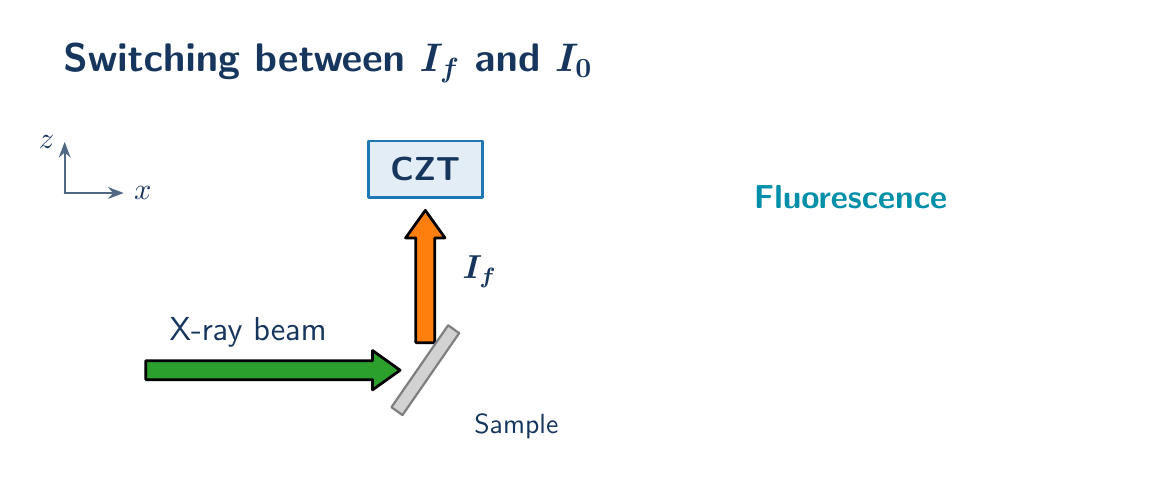
\begin{tikzpicture}[x=1cm,y=1cm,line join=round,line cap=round,
 every node/.style={font=\sffamily\fontsize{12}{14}\selectfont,text=ink},
]
\newcommand{\BeamArrow}[4]{%
  \begin{scope}
    \coordinate (beamStart) at #3;
    \coordinate (beamEnd) at #4;
    \path let \p1 = ($(beamEnd)-(beamStart)$),
      \n1 = {atan2(\y1,\x1)}, \n2 = {veclen(\x1,\y1)} in
      \pgfextra{\xdef\beamAngle{\n1}\xdef\beamLength{\n2}};
    \begin{scope}[shift={(beamStart)},rotate=\beamAngle]
      \path[fill=#1,draw=black,opacity=#2,line width=.35mm,line join=round]
        (0,-1.2mm) -- (\beamLength-3.5mm,-1.2mm)
        -- (\beamLength-3.5mm,-2.5mm) -- (\beamLength,0)
        -- (\beamLength-3.5mm,2.5mm) -- (\beamLength-3.5mm,1.2mm)
        -- (0,1.2mm) -- cycle;
    \end{scope}
  \end{scope}
}
\path[use as bounding box] (-1.05,-1.25) rectangle (12.8878,4.35);
\node[anchor=west,font=\sffamily\bfseries\fontsize{14}{17}\selectfont] at (-.72,3.9) {Switching between $\bm{I_f}$ and $\bm{I_0}$};
\draw[ink!75,line width=.8pt,-{Stealth[length=2mm]}] (-.58,2.25) -- (.17,2.25) node[anchor=west,font=\sffamily\fontsize{11}{13}\selectfont] {$x$};
\draw[ink!75,line width=.8pt,-{Stealth[length=2mm]}] (-.58,2.25) -- (-.58,2.9) node[anchor=east,font=\sffamily\fontsize{11}{13}\selectfont] {$z$};
\BeamArrow{beamgreen}{1.0000}{(.45,0)}{(3.68,0)}
\node at (1.75,.48) {X-ray beam};
\BeamArrow{beamgreen}{0.0000}{(.45,0)}{(5.98,0)}
\BeamArrow{fluororange}{1.0000}{(4,.35)}{(4,2.03)}
\node[opacity=1.0000,anchor=west] at (4.35,1.25) {$\bm{I_f}$};
\node[opacity=0.0000] at (5.25,.48) {$\bm{I_0}$};
\begin{scope}[shift={(4,0.0000)}]
\path[draw=samplegray,fill=samplegray!35,line width=.8pt] (-.43,-.47) -- (-.29,-.57) -- (.43,.47) -- (.29,.57) -- cycle;
\end{scope}
\node[anchor=west,font=\sffamily\fontsize{10}{12}\selectfont] at (4.5,-0.7200) {Sample};
\begin{scope}[shift={(4.0000,2.5500)},rotate=-0.0000,transform shape]
\node[draw=detectorblue,fill=detectorblue!13,line width=1pt,minimum width=1.45cm,minimum height=.72cm,inner sep=2pt,font=\sffamily\bfseries\fontsize{13}{15}\selectfont] {CZT};
\end{scope}
\node[opacity=1.0000,font=\sffamily\bfseries\fontsize{13}{15}\selectfont,text=motioncyan] at (9.4,2.2) {Fluorescence};
\node[opacity=0.0000,font=\sffamily\bfseries\fontsize{13}{15}\selectfont,text=motioncyan] at (9.4,2.2) {Incident beam};
\end{tikzpicture}
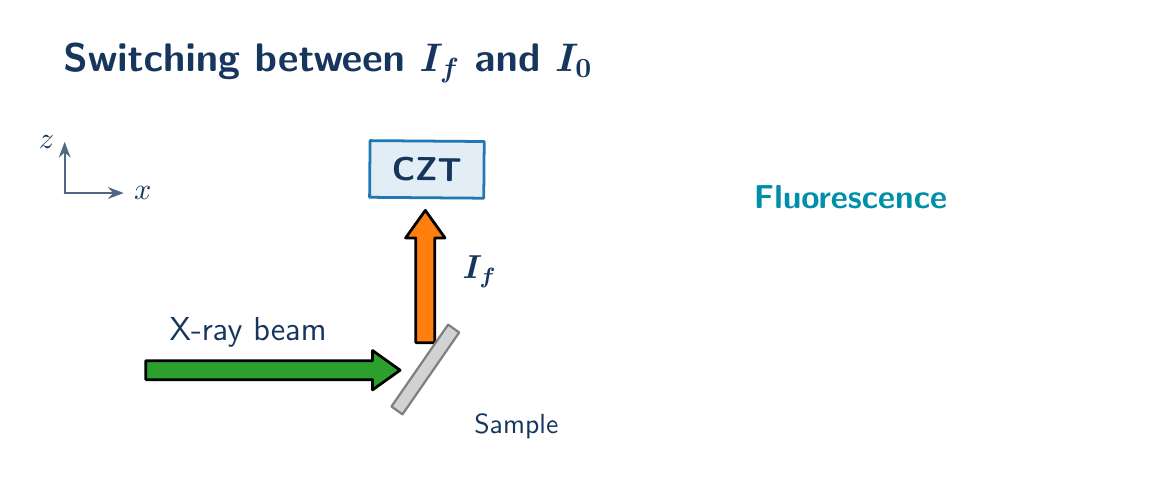
\begin{tikzpicture}[x=1cm,y=1cm,line join=round,line cap=round,
 every node/.style={font=\sffamily\fontsize{12}{14}\selectfont,text=ink},
]
\newcommand{\BeamArrow}[4]{%
  \begin{scope}
    \coordinate (beamStart) at #3;
    \coordinate (beamEnd) at #4;
    \path let \p1 = ($(beamEnd)-(beamStart)$),
      \n1 = {atan2(\y1,\x1)}, \n2 = {veclen(\x1,\y1)} in
      \pgfextra{\xdef\beamAngle{\n1}\xdef\beamLength{\n2}};
    \begin{scope}[shift={(beamStart)},rotate=\beamAngle]
      \path[fill=#1,draw=black,opacity=#2,line width=.35mm,line join=round]
        (0,-1.2mm) -- (\beamLength-3.5mm,-1.2mm)
        -- (\beamLength-3.5mm,-2.5mm) -- (\beamLength,0)
        -- (\beamLength-3.5mm,2.5mm) -- (\beamLength-3.5mm,1.2mm)
        -- (0,1.2mm) -- cycle;
    \end{scope}
  \end{scope}
}
\path[use as bounding box] (-1.05,-1.25) rectangle (12.8878,4.35);
\node[anchor=west,font=\sffamily\bfseries\fontsize{14}{17}\selectfont] at (-.72,3.9) {Switching between $\bm{I_f}$ and $\bm{I_0}$};
\draw[ink!75,line width=.8pt,-{Stealth[length=2mm]}] (-.58,2.25) -- (.17,2.25) node[anchor=west,font=\sffamily\fontsize{11}{13}\selectfont] {$x$};
\draw[ink!75,line width=.8pt,-{Stealth[length=2mm]}] (-.58,2.25) -- (-.58,2.9) node[anchor=east,font=\sffamily\fontsize{11}{13}\selectfont] {$z$};
\BeamArrow{beamgreen}{1.0000}{(.45,0)}{(3.68,0)}
\node at (1.75,.48) {X-ray beam};
\BeamArrow{beamgreen}{0.0000}{(.45,0)}{(5.98,0)}
\BeamArrow{fluororange}{0.9995}{(4,.35)}{(4,2.03)}
\node[opacity=0.9995,anchor=west] at (4.35,1.25) {$\bm{I_f}$};
\node[opacity=0.0000] at (5.25,.48) {$\bm{I_0}$};
\begin{scope}[shift={(4,0.0089)}]
\path[draw=samplegray,fill=samplegray!35,line width=.8pt] (-.43,-.47) -- (-.29,-.57) -- (.43,.47) -- (.29,.57) -- cycle;
\end{scope}
\node[anchor=west,font=\sffamily\fontsize{10}{12}\selectfont] at (4.5,-0.7111) {Sample};
\begin{scope}[shift={(4.0203,2.5499)},rotate=-0.4557,transform shape]
\node[draw=detectorblue,fill=detectorblue!13,line width=1pt,minimum width=1.45cm,minimum height=.72cm,inner sep=2pt,font=\sffamily\bfseries\fontsize{13}{15}\selectfont] {CZT};
\end{scope}
\node[opacity=0.9995,font=\sffamily\bfseries\fontsize{13}{15}\selectfont,text=motioncyan] at (9.4,2.2) {Fluorescence};
\node[opacity=0.0000,font=\sffamily\bfseries\fontsize{13}{15}\selectfont,text=motioncyan] at (9.4,2.2) {Incident beam};
\end{tikzpicture}
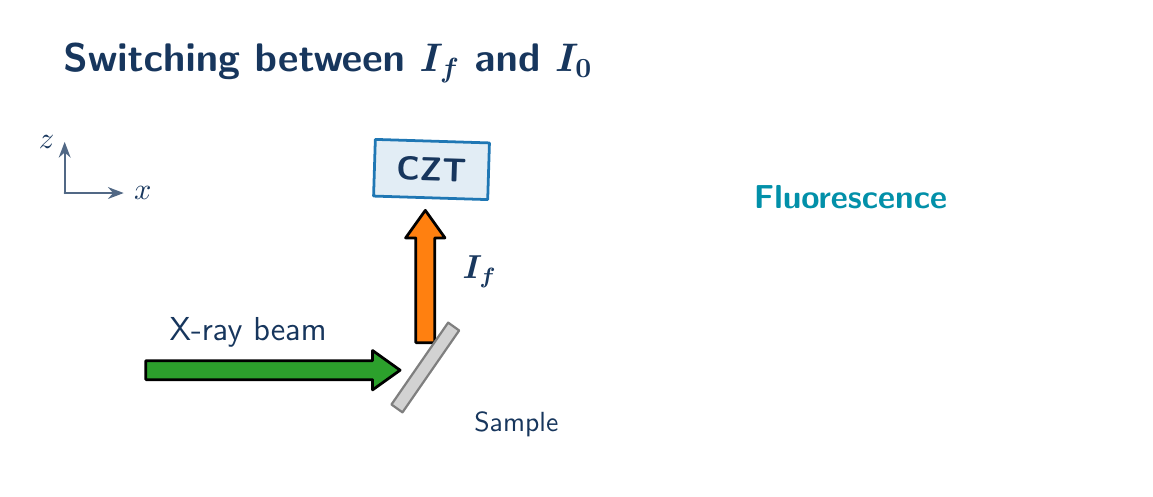
\begin{tikzpicture}[x=1cm,y=1cm,line join=round,line cap=round,
 every node/.style={font=\sffamily\fontsize{12}{14}\selectfont,text=ink},
]
\newcommand{\BeamArrow}[4]{%
  \begin{scope}
    \coordinate (beamStart) at #3;
    \coordinate (beamEnd) at #4;
    \path let \p1 = ($(beamEnd)-(beamStart)$),
      \n1 = {atan2(\y1,\x1)}, \n2 = {veclen(\x1,\y1)} in
      \pgfextra{\xdef\beamAngle{\n1}\xdef\beamLength{\n2}};
    \begin{scope}[shift={(beamStart)},rotate=\beamAngle]
      \path[fill=#1,draw=black,opacity=#2,line width=.35mm,line join=round]
        (0,-1.2mm) -- (\beamLength-3.5mm,-1.2mm)
        -- (\beamLength-3.5mm,-2.5mm) -- (\beamLength,0)
        -- (\beamLength-3.5mm,2.5mm) -- (\beamLength-3.5mm,1.2mm)
        -- (0,1.2mm) -- cycle;
    \end{scope}
  \end{scope}
}
\path[use as bounding box] (-1.05,-1.25) rectangle (12.8878,4.35);
\node[anchor=west,font=\sffamily\bfseries\fontsize{14}{17}\selectfont] at (-.72,3.9) {Switching between $\bm{I_f}$ and $\bm{I_0}$};
\draw[ink!75,line width=.8pt,-{Stealth[length=2mm]}] (-.58,2.25) -- (.17,2.25) node[anchor=west,font=\sffamily\fontsize{11}{13}\selectfont] {$x$};
\draw[ink!75,line width=.8pt,-{Stealth[length=2mm]}] (-.58,2.25) -- (-.58,2.9) node[anchor=east,font=\sffamily\fontsize{11}{13}\selectfont] {$z$};
\BeamArrow{beamgreen}{1.0000}{(.45,0)}{(3.68,0)}
\node at (1.75,.48) {X-ray beam};
\BeamArrow{beamgreen}{0.0000}{(.45,0)}{(5.98,0)}
\BeamArrow{fluororange}{0.9922}{(4,.35)}{(4,2.03)}
\node[opacity=0.9922,anchor=west] at (4.35,1.25) {$\bm{I_f}$};
\node[opacity=0.0000] at (5.25,.48) {$\bm{I_0}$};
\begin{scope}[shift={(4,0.0344)}]
\path[draw=samplegray,fill=samplegray!35,line width=.8pt] (-.43,-.47) -- (-.29,-.57) -- (.43,.47) -- (.29,.57) -- cycle;
\end{scope}
\node[anchor=west,font=\sffamily\fontsize{10}{12}\selectfont] at (4.5,-0.6856) {Sample};
\begin{scope}[shift={(4.0788,2.5488)},rotate=-1.7708,transform shape]
\node[draw=detectorblue,fill=detectorblue!13,line width=1pt,minimum width=1.45cm,minimum height=.72cm,inner sep=2pt,font=\sffamily\bfseries\fontsize{13}{15}\selectfont] {CZT};
\end{scope}
\node[opacity=0.9922,font=\sffamily\bfseries\fontsize{13}{15}\selectfont,text=motioncyan] at (9.4,2.2) {Fluorescence};
\node[opacity=0.0000,font=\sffamily\bfseries\fontsize{13}{15}\selectfont,text=motioncyan] at (9.4,2.2) {Incident beam};
\end{tikzpicture}
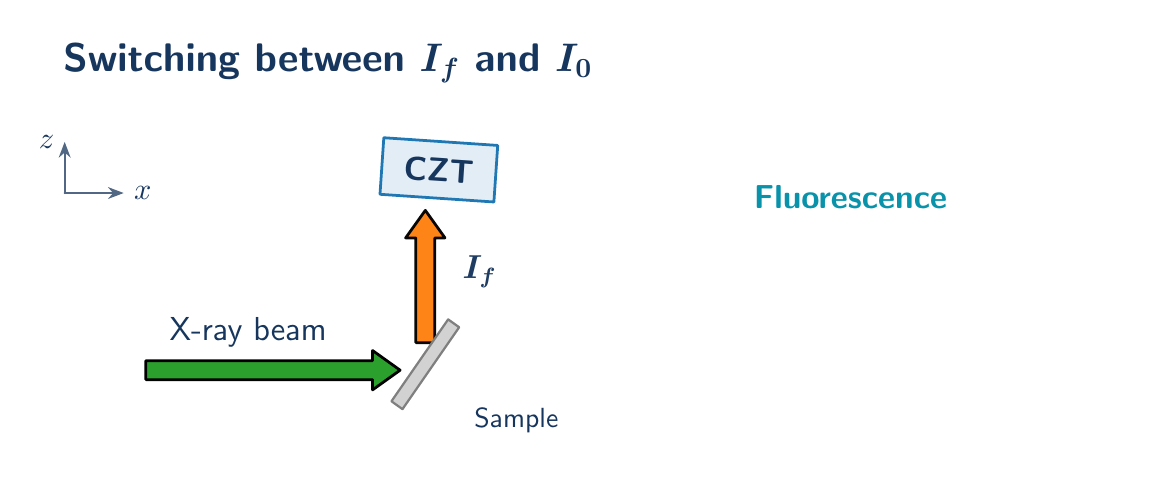
\begin{tikzpicture}[x=1cm,y=1cm,line join=round,line cap=round,
 every node/.style={font=\sffamily\fontsize{12}{14}\selectfont,text=ink},
]
\newcommand{\BeamArrow}[4]{%
  \begin{scope}
    \coordinate (beamStart) at #3;
    \coordinate (beamEnd) at #4;
    \path let \p1 = ($(beamEnd)-(beamStart)$),
      \n1 = {atan2(\y1,\x1)}, \n2 = {veclen(\x1,\y1)} in
      \pgfextra{\xdef\beamAngle{\n1}\xdef\beamLength{\n2}};
    \begin{scope}[shift={(beamStart)},rotate=\beamAngle]
      \path[fill=#1,draw=black,opacity=#2,line width=.35mm,line join=round]
        (0,-1.2mm) -- (\beamLength-3.5mm,-1.2mm)
        -- (\beamLength-3.5mm,-2.5mm) -- (\beamLength,0)
        -- (\beamLength-3.5mm,2.5mm) -- (\beamLength-3.5mm,1.2mm)
        -- (0,1.2mm) -- cycle;
    \end{scope}
  \end{scope}
}
\path[use as bounding box] (-1.05,-1.25) rectangle (12.8878,4.35);
\node[anchor=west,font=\sffamily\bfseries\fontsize{14}{17}\selectfont] at (-.72,3.9) {Switching between $\bm{I_f}$ and $\bm{I_0}$};
\draw[ink!75,line width=.8pt,-{Stealth[length=2mm]}] (-.58,2.25) -- (.17,2.25) node[anchor=west,font=\sffamily\fontsize{11}{13}\selectfont] {$x$};
\draw[ink!75,line width=.8pt,-{Stealth[length=2mm]}] (-.58,2.25) -- (-.58,2.9) node[anchor=east,font=\sffamily\fontsize{11}{13}\selectfont] {$z$};
\BeamArrow{beamgreen}{1.0000}{(.45,0)}{(3.68,0)}
\node at (1.75,.48) {X-ray beam};
\BeamArrow{beamgreen}{0.0000}{(.45,0)}{(5.98,0)}
\BeamArrow{fluororange}{0.9645}{(4,.35)}{(4,2.03)}
\node[opacity=0.9645,anchor=west] at (4.35,1.25) {$\bm{I_f}$};
\node[opacity=0.0000] at (5.25,.48) {$\bm{I_0}$};
\begin{scope}[shift={(4,0.0752)}]
\path[draw=samplegray,fill=samplegray!35,line width=.8pt] (-.43,-.47) -- (-.29,-.57) -- (.43,.47) -- (.29,.57) -- cycle;
\end{scope}
\node[anchor=west,font=\sffamily\fontsize{10}{12}\selectfont] at (4.5,-0.6448) {Sample};
\begin{scope}[shift={(4.1720,2.5442)},rotate=-3.8672,transform shape]
\node[draw=detectorblue,fill=detectorblue!13,line width=1pt,minimum width=1.45cm,minimum height=.72cm,inner sep=2pt,font=\sffamily\bfseries\fontsize{13}{15}\selectfont] {CZT};
\end{scope}
\node[opacity=0.9645,font=\sffamily\bfseries\fontsize{13}{15}\selectfont,text=motioncyan] at (9.4,2.2) {Fluorescence};
\node[opacity=0.0000,font=\sffamily\bfseries\fontsize{13}{15}\selectfont,text=motioncyan] at (9.4,2.2) {Incident beam};
\end{tikzpicture}
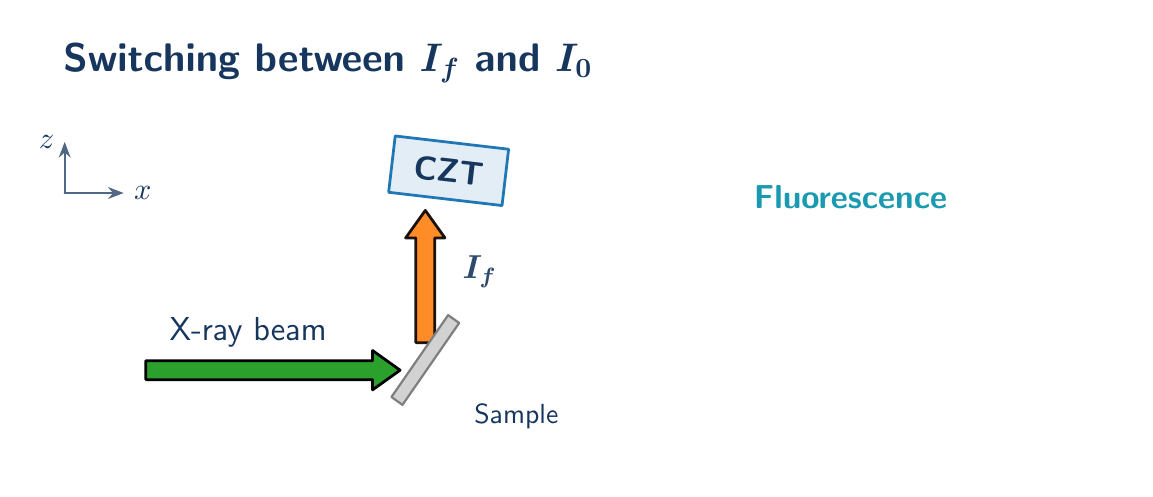
\begin{tikzpicture}[x=1cm,y=1cm,line join=round,line cap=round,
 every node/.style={font=\sffamily\fontsize{12}{14}\selectfont,text=ink},
]
\newcommand{\BeamArrow}[4]{%
  \begin{scope}
    \coordinate (beamStart) at #3;
    \coordinate (beamEnd) at #4;
    \path let \p1 = ($(beamEnd)-(beamStart)$),
      \n1 = {atan2(\y1,\x1)}, \n2 = {veclen(\x1,\y1)} in
      \pgfextra{\xdef\beamAngle{\n1}\xdef\beamLength{\n2}};
    \begin{scope}[shift={(beamStart)},rotate=\beamAngle]
      \path[fill=#1,draw=black,opacity=#2,line width=.35mm,line join=round]
        (0,-1.2mm) -- (\beamLength-3.5mm,-1.2mm)
        -- (\beamLength-3.5mm,-2.5mm) -- (\beamLength,0)
        -- (\beamLength-3.5mm,2.5mm) -- (\beamLength-3.5mm,1.2mm)
        -- (0,1.2mm) -- cycle;
    \end{scope}
  \end{scope}
}
\path[use as bounding box] (-1.05,-1.25) rectangle (12.8878,4.35);
\node[anchor=west,font=\sffamily\bfseries\fontsize{14}{17}\selectfont] at (-.72,3.9) {Switching between $\bm{I_f}$ and $\bm{I_0}$};
\draw[ink!75,line width=.8pt,-{Stealth[length=2mm]}] (-.58,2.25) -- (.17,2.25) node[anchor=west,font=\sffamily\fontsize{11}{13}\selectfont] {$x$};
\draw[ink!75,line width=.8pt,-{Stealth[length=2mm]}] (-.58,2.25) -- (-.58,2.9) node[anchor=east,font=\sffamily\fontsize{11}{13}\selectfont] {$z$};
\BeamArrow{beamgreen}{1.0000}{(.45,0)}{(3.68,0)}
\node at (1.75,.48) {X-ray beam};
\BeamArrow{beamgreen}{0.0000}{(.45,0)}{(5.98,0)}
\BeamArrow{fluororange}{0.9008}{(4,.35)}{(4,2.03)}
\node[opacity=0.9008,anchor=west] at (4.35,1.25) {$\bm{I_f}$};
\node[opacity=0.0000] at (5.25,.48) {$\bm{I_0}$};
\begin{scope}[shift={(4,0.1296)}]
\path[draw=samplegray,fill=samplegray!35,line width=.8pt] (-.43,-.47) -- (-.29,-.57) -- (.43,.47) -- (.29,.57) -- cycle;
\end{scope}
\node[anchor=west,font=\sffamily\fontsize{10}{12}\selectfont] at (4.5,-0.5904) {Sample};
\begin{scope}[shift={(4.2960,2.5328)},rotate=-6.6667,transform shape]
\node[draw=detectorblue,fill=detectorblue!13,line width=1pt,minimum width=1.45cm,minimum height=.72cm,inner sep=2pt,font=\sffamily\bfseries\fontsize{13}{15}\selectfont] {CZT};
\end{scope}
\node[opacity=0.9008,font=\sffamily\bfseries\fontsize{13}{15}\selectfont,text=motioncyan] at (9.4,2.2) {Fluorescence};
\node[opacity=0.0000,font=\sffamily\bfseries\fontsize{13}{15}\selectfont,text=motioncyan] at (9.4,2.2) {Incident beam};
\end{tikzpicture}
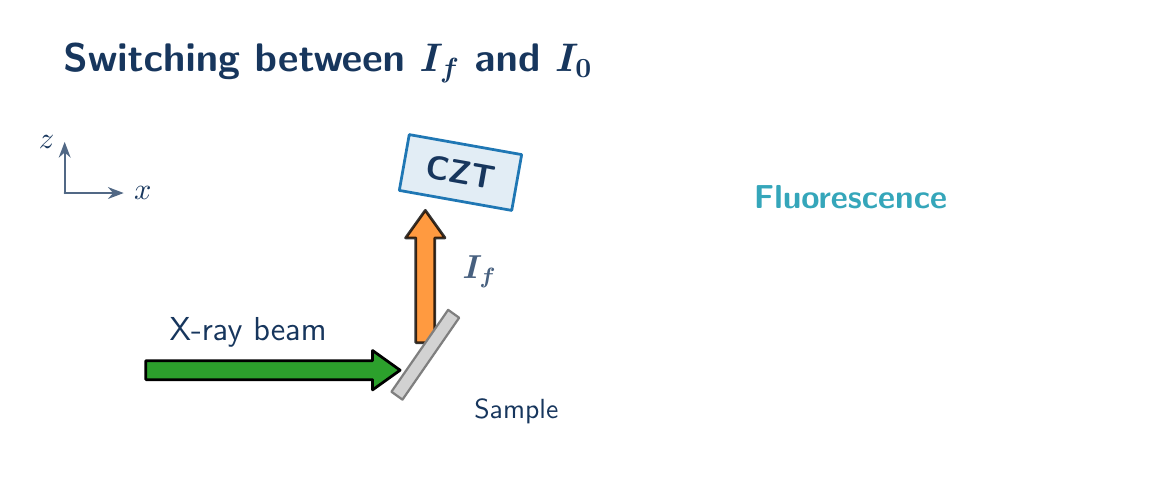
\begin{tikzpicture}[x=1cm,y=1cm,line join=round,line cap=round,
 every node/.style={font=\sffamily\fontsize{12}{14}\selectfont,text=ink},
]
\newcommand{\BeamArrow}[4]{%
  \begin{scope}
    \coordinate (beamStart) at #3;
    \coordinate (beamEnd) at #4;
    \path let \p1 = ($(beamEnd)-(beamStart)$),
      \n1 = {atan2(\y1,\x1)}, \n2 = {veclen(\x1,\y1)} in
      \pgfextra{\xdef\beamAngle{\n1}\xdef\beamLength{\n2}};
    \begin{scope}[shift={(beamStart)},rotate=\beamAngle]
      \path[fill=#1,draw=black,opacity=#2,line width=.35mm,line join=round]
        (0,-1.2mm) -- (\beamLength-3.5mm,-1.2mm)
        -- (\beamLength-3.5mm,-2.5mm) -- (\beamLength,0)
        -- (\beamLength-3.5mm,2.5mm) -- (\beamLength-3.5mm,1.2mm)
        -- (0,1.2mm) -- cycle;
    \end{scope}
  \end{scope}
}
\path[use as bounding box] (-1.05,-1.25) rectangle (12.8878,4.35);
\node[anchor=west,font=\sffamily\bfseries\fontsize{14}{17}\selectfont] at (-.72,3.9) {Switching between $\bm{I_f}$ and $\bm{I_0}$};
\draw[ink!75,line width=.8pt,-{Stealth[length=2mm]}] (-.58,2.25) -- (.17,2.25) node[anchor=west,font=\sffamily\fontsize{11}{13}\selectfont] {$x$};
\draw[ink!75,line width=.8pt,-{Stealth[length=2mm]}] (-.58,2.25) -- (-.58,2.9) node[anchor=east,font=\sffamily\fontsize{11}{13}\selectfont] {$z$};
\BeamArrow{beamgreen}{1.0000}{(.45,0)}{(3.68,0)}
\node at (1.75,.48) {X-ray beam};
\BeamArrow{beamgreen}{0.0000}{(.45,0)}{(5.98,0)}
\BeamArrow{fluororange}{0.7902}{(4,.35)}{(4,2.03)}
\node[opacity=0.7902,anchor=west] at (4.35,1.25) {$\bm{I_f}$};
\node[opacity=0.0000] at (5.25,.48) {$\bm{I_0}$};
\begin{scope}[shift={(4,0.1962)}]
\path[draw=samplegray,fill=samplegray!35,line width=.8pt] (-.43,-.47) -- (-.29,-.57) -- (.43,.47) -- (.29,.57) -- cycle;
\end{scope}
\node[anchor=west,font=\sffamily\fontsize{10}{12}\selectfont] at (4.5,-0.5238) {Sample};
\begin{scope}[shift={(4.4468,2.5106)},rotate=-10.0911,transform shape]
\node[draw=detectorblue,fill=detectorblue!13,line width=1pt,minimum width=1.45cm,minimum height=.72cm,inner sep=2pt,font=\sffamily\bfseries\fontsize{13}{15}\selectfont] {CZT};
\end{scope}
\node[opacity=0.7902,font=\sffamily\bfseries\fontsize{13}{15}\selectfont,text=motioncyan] at (9.4,2.2) {Fluorescence};
\node[opacity=0.0000,font=\sffamily\bfseries\fontsize{13}{15}\selectfont,text=motioncyan] at (9.4,2.2) {Incident beam};
\end{tikzpicture}
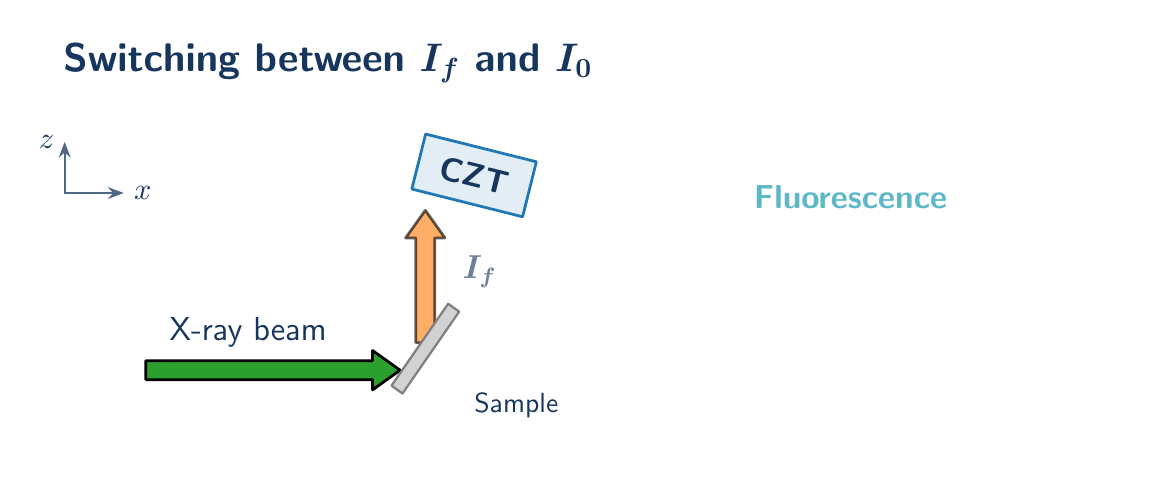
\begin{tikzpicture}[x=1cm,y=1cm,line join=round,line cap=round,
 every node/.style={font=\sffamily\fontsize{12}{14}\selectfont,text=ink},
]
\newcommand{\BeamArrow}[4]{%
  \begin{scope}
    \coordinate (beamStart) at #3;
    \coordinate (beamEnd) at #4;
    \path let \p1 = ($(beamEnd)-(beamStart)$),
      \n1 = {atan2(\y1,\x1)}, \n2 = {veclen(\x1,\y1)} in
      \pgfextra{\xdef\beamAngle{\n1}\xdef\beamLength{\n2}};
    \begin{scope}[shift={(beamStart)},rotate=\beamAngle]
      \path[fill=#1,draw=black,opacity=#2,line width=.35mm,line join=round]
        (0,-1.2mm) -- (\beamLength-3.5mm,-1.2mm)
        -- (\beamLength-3.5mm,-2.5mm) -- (\beamLength,0)
        -- (\beamLength-3.5mm,2.5mm) -- (\beamLength-3.5mm,1.2mm)
        -- (0,1.2mm) -- cycle;
    \end{scope}
  \end{scope}
}
\path[use as bounding box] (-1.05,-1.25) rectangle (12.8878,4.35);
\node[anchor=west,font=\sffamily\bfseries\fontsize{14}{17}\selectfont] at (-.72,3.9) {Switching between $\bm{I_f}$ and $\bm{I_0}$};
\draw[ink!75,line width=.8pt,-{Stealth[length=2mm]}] (-.58,2.25) -- (.17,2.25) node[anchor=west,font=\sffamily\fontsize{11}{13}\selectfont] {$x$};
\draw[ink!75,line width=.8pt,-{Stealth[length=2mm]}] (-.58,2.25) -- (-.58,2.9) node[anchor=east,font=\sffamily\fontsize{11}{13}\selectfont] {$z$};
\BeamArrow{beamgreen}{1.0000}{(.45,0)}{(3.68,0)}
\node at (1.75,.48) {X-ray beam};
\BeamArrow{beamgreen}{0.0000}{(.45,0)}{(5.98,0)}
\BeamArrow{fluororange}{0.6318}{(4,.35)}{(4,2.03)}
\node[opacity=0.6318,anchor=west] at (4.35,1.25) {$\bm{I_f}$};
\node[opacity=0.0000] at (5.25,.48) {$\bm{I_0}$};
\begin{scope}[shift={(4,0.2734)}]
\path[draw=samplegray,fill=samplegray!35,line width=.8pt] (-.43,-.47) -- (-.29,-.57) -- (.43,.47) -- (.29,.57) -- cycle;
\end{scope}
\node[anchor=west,font=\sffamily\fontsize{10}{12}\selectfont] at (4.5,-0.4466) {Sample};
\begin{scope}[shift={(4.6196,2.4736)},rotate=-14.0625,transform shape]
\node[draw=detectorblue,fill=detectorblue!13,line width=1pt,minimum width=1.45cm,minimum height=.72cm,inner sep=2pt,font=\sffamily\bfseries\fontsize{13}{15}\selectfont] {CZT};
\end{scope}
\node[opacity=0.6318,font=\sffamily\bfseries\fontsize{13}{15}\selectfont,text=motioncyan] at (9.4,2.2) {Fluorescence};
\node[opacity=0.0000,font=\sffamily\bfseries\fontsize{13}{15}\selectfont,text=motioncyan] at (9.4,2.2) {Incident beam};
\end{tikzpicture}
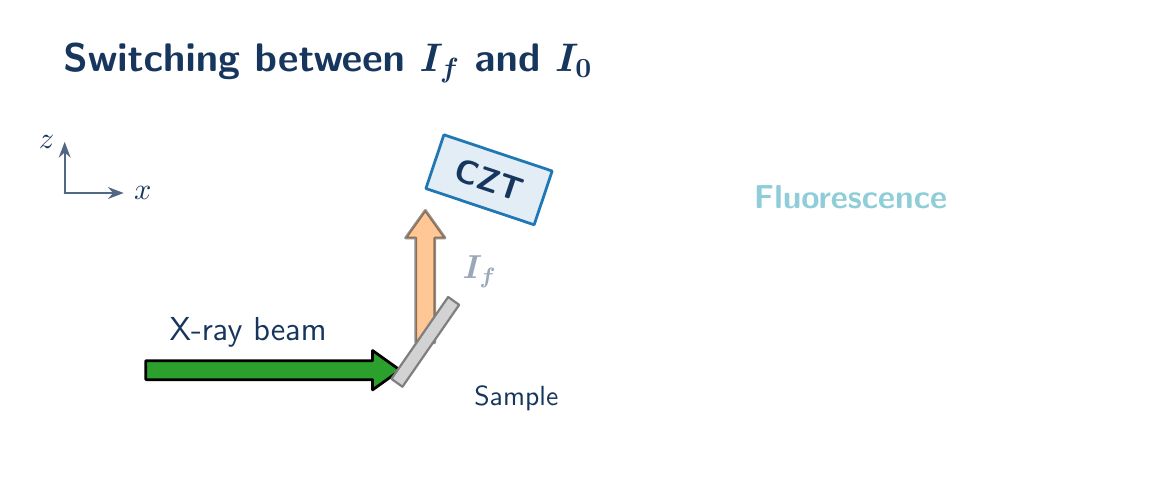
\begin{tikzpicture}[x=1cm,y=1cm,line join=round,line cap=round,
 every node/.style={font=\sffamily\fontsize{12}{14}\selectfont,text=ink},
]
\newcommand{\BeamArrow}[4]{%
  \begin{scope}
    \coordinate (beamStart) at #3;
    \coordinate (beamEnd) at #4;
    \path let \p1 = ($(beamEnd)-(beamStart)$),
      \n1 = {atan2(\y1,\x1)}, \n2 = {veclen(\x1,\y1)} in
      \pgfextra{\xdef\beamAngle{\n1}\xdef\beamLength{\n2}};
    \begin{scope}[shift={(beamStart)},rotate=\beamAngle]
      \path[fill=#1,draw=black,opacity=#2,line width=.35mm,line join=round]
        (0,-1.2mm) -- (\beamLength-3.5mm,-1.2mm)
        -- (\beamLength-3.5mm,-2.5mm) -- (\beamLength,0)
        -- (\beamLength-3.5mm,2.5mm) -- (\beamLength-3.5mm,1.2mm)
        -- (0,1.2mm) -- cycle;
    \end{scope}
  \end{scope}
}
\path[use as bounding box] (-1.05,-1.25) rectangle (12.8878,4.35);
\node[anchor=west,font=\sffamily\bfseries\fontsize{14}{17}\selectfont] at (-.72,3.9) {Switching between $\bm{I_f}$ and $\bm{I_0}$};
\draw[ink!75,line width=.8pt,-{Stealth[length=2mm]}] (-.58,2.25) -- (.17,2.25) node[anchor=west,font=\sffamily\fontsize{11}{13}\selectfont] {$x$};
\draw[ink!75,line width=.8pt,-{Stealth[length=2mm]}] (-.58,2.25) -- (-.58,2.9) node[anchor=east,font=\sffamily\fontsize{11}{13}\selectfont] {$z$};
\BeamArrow{beamgreen}{1.0000}{(.45,0)}{(3.68,0)}
\node at (1.75,.48) {X-ray beam};
\BeamArrow{beamgreen}{0.0000}{(.45,0)}{(5.98,0)}
\BeamArrow{fluororange}{0.4386}{(4,.35)}{(4,2.03)}
\node[opacity=0.4386,anchor=west] at (4.35,1.25) {$\bm{I_f}$};
\node[opacity=0.0000] at (5.25,.48) {$\bm{I_0}$};
\begin{scope}[shift={(4,0.3598)}]
\path[draw=samplegray,fill=samplegray!35,line width=.8pt] (-.43,-.47) -- (-.29,-.57) -- (.43,.47) -- (.29,.57) -- cycle;
\end{scope}
\node[anchor=west,font=\sffamily\fontsize{10}{12}\selectfont] at (4.5,-0.3602) {Sample};
\begin{scope}[shift={(4.8092,2.4182)},rotate=-18.5026,transform shape]
\node[draw=detectorblue,fill=detectorblue!13,line width=1pt,minimum width=1.45cm,minimum height=.72cm,inner sep=2pt,font=\sffamily\bfseries\fontsize{13}{15}\selectfont] {CZT};
\end{scope}
\node[opacity=0.4386,font=\sffamily\bfseries\fontsize{13}{15}\selectfont,text=motioncyan] at (9.4,2.2) {Fluorescence};
\node[opacity=0.0000,font=\sffamily\bfseries\fontsize{13}{15}\selectfont,text=motioncyan] at (9.4,2.2) {Incident beam};
\end{tikzpicture}
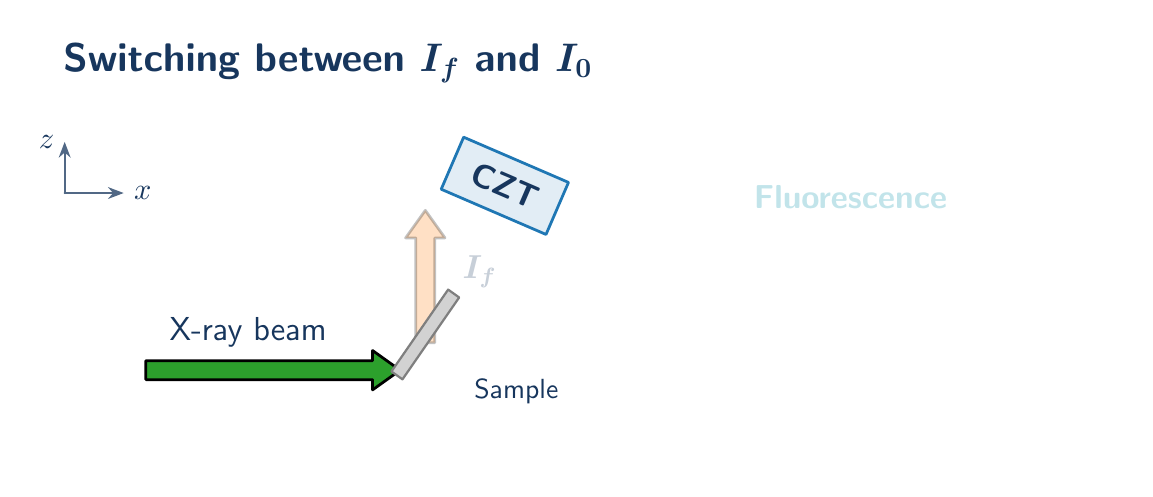
\begin{tikzpicture}[x=1cm,y=1cm,line join=round,line cap=round,
 every node/.style={font=\sffamily\fontsize{12}{14}\selectfont,text=ink},
]
\newcommand{\BeamArrow}[4]{%
  \begin{scope}
    \coordinate (beamStart) at #3;
    \coordinate (beamEnd) at #4;
    \path let \p1 = ($(beamEnd)-(beamStart)$),
      \n1 = {atan2(\y1,\x1)}, \n2 = {veclen(\x1,\y1)} in
      \pgfextra{\xdef\beamAngle{\n1}\xdef\beamLength{\n2}};
    \begin{scope}[shift={(beamStart)},rotate=\beamAngle]
      \path[fill=#1,draw=black,opacity=#2,line width=.35mm,line join=round]
        (0,-1.2mm) -- (\beamLength-3.5mm,-1.2mm)
        -- (\beamLength-3.5mm,-2.5mm) -- (\beamLength,0)
        -- (\beamLength-3.5mm,2.5mm) -- (\beamLength-3.5mm,1.2mm)
        -- (0,1.2mm) -- cycle;
    \end{scope}
  \end{scope}
}
\path[use as bounding box] (-1.05,-1.25) rectangle (12.8878,4.35);
\node[anchor=west,font=\sffamily\bfseries\fontsize{14}{17}\selectfont] at (-.72,3.9) {Switching between $\bm{I_f}$ and $\bm{I_0}$};
\draw[ink!75,line width=.8pt,-{Stealth[length=2mm]}] (-.58,2.25) -- (.17,2.25) node[anchor=west,font=\sffamily\fontsize{11}{13}\selectfont] {$x$};
\draw[ink!75,line width=.8pt,-{Stealth[length=2mm]}] (-.58,2.25) -- (-.58,2.9) node[anchor=east,font=\sffamily\fontsize{11}{13}\selectfont] {$z$};
\BeamArrow{beamgreen}{1.0000}{(.45,0)}{(3.68,0)}
\node at (1.75,.48) {X-ray beam};
\BeamArrow{beamgreen}{0.0000}{(.45,0)}{(5.98,0)}
\BeamArrow{fluororange}{0.2387}{(4,.35)}{(4,2.03)}
\node[opacity=0.2387,anchor=west] at (4.35,1.25) {$\bm{I_f}$};
\node[opacity=0.0000] at (5.25,.48) {$\bm{I_0}$};
\begin{scope}[shift={(4,0.4537)}]
\path[draw=samplegray,fill=samplegray!35,line width=.8pt] (-.43,-.47) -- (-.29,-.57) -- (.43,.47) -- (.29,.57) -- cycle;
\end{scope}
\node[anchor=west,font=\sffamily\fontsize{10}{12}\selectfont] at (4.5,-0.2663) {Sample};
\begin{scope}[shift={(5.0100,2.3415)},rotate=-23.3333,transform shape]
\node[draw=detectorblue,fill=detectorblue!13,line width=1pt,minimum width=1.45cm,minimum height=.72cm,inner sep=2pt,font=\sffamily\bfseries\fontsize{13}{15}\selectfont] {CZT};
\end{scope}
\node[opacity=0.2387,font=\sffamily\bfseries\fontsize{13}{15}\selectfont,text=motioncyan] at (9.4,2.2) {Fluorescence};
\node[opacity=0.0000,font=\sffamily\bfseries\fontsize{13}{15}\selectfont,text=motioncyan] at (9.4,2.2) {Incident beam};
\end{tikzpicture}
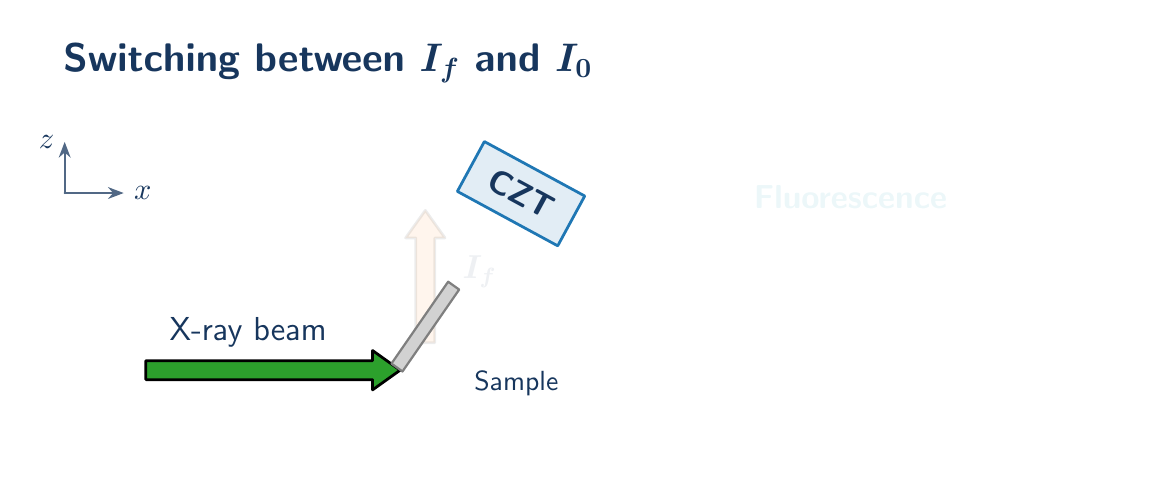
\begin{tikzpicture}[x=1cm,y=1cm,line join=round,line cap=round,
 every node/.style={font=\sffamily\fontsize{12}{14}\selectfont,text=ink},
]
\newcommand{\BeamArrow}[4]{%
  \begin{scope}
    \coordinate (beamStart) at #3;
    \coordinate (beamEnd) at #4;
    \path let \p1 = ($(beamEnd)-(beamStart)$),
      \n1 = {atan2(\y1,\x1)}, \n2 = {veclen(\x1,\y1)} in
      \pgfextra{\xdef\beamAngle{\n1}\xdef\beamLength{\n2}};
    \begin{scope}[shift={(beamStart)},rotate=\beamAngle]
      \path[fill=#1,draw=black,opacity=#2,line width=.35mm,line join=round]
        (0,-1.2mm) -- (\beamLength-3.5mm,-1.2mm)
        -- (\beamLength-3.5mm,-2.5mm) -- (\beamLength,0)
        -- (\beamLength-3.5mm,2.5mm) -- (\beamLength-3.5mm,1.2mm)
        -- (0,1.2mm) -- cycle;
    \end{scope}
  \end{scope}
}
\path[use as bounding box] (-1.05,-1.25) rectangle (12.8878,4.35);
\node[anchor=west,font=\sffamily\bfseries\fontsize{14}{17}\selectfont] at (-.72,3.9) {Switching between $\bm{I_f}$ and $\bm{I_0}$};
\draw[ink!75,line width=.8pt,-{Stealth[length=2mm]}] (-.58,2.25) -- (.17,2.25) node[anchor=west,font=\sffamily\fontsize{11}{13}\selectfont] {$x$};
\draw[ink!75,line width=.8pt,-{Stealth[length=2mm]}] (-.58,2.25) -- (-.58,2.9) node[anchor=east,font=\sffamily\fontsize{11}{13}\selectfont] {$z$};
\BeamArrow{beamgreen}{1.0000}{(.45,0)}{(3.68,0)}
\node at (1.75,.48) {X-ray beam};
\BeamArrow{beamgreen}{0.0000}{(.45,0)}{(5.98,0)}
\BeamArrow{fluororange}{0.0746}{(4,.35)}{(4,2.03)}
\node[opacity=0.0746,anchor=west] at (4.35,1.25) {$\bm{I_f}$};
\node[opacity=0.0000] at (5.25,.48) {$\bm{I_0}$};
\begin{scope}[shift={(4,0.5537)}]
\path[draw=samplegray,fill=samplegray!35,line width=.8pt] (-.43,-.47) -- (-.29,-.57) -- (.43,.47) -- (.29,.57) -- cycle;
\end{scope}
\node[anchor=west,font=\sffamily\fontsize{10}{12}\selectfont] at (4.5,-0.1663) {Sample};
\begin{scope}[shift={(5.2158,2.2415)},rotate=-28.4766,transform shape]
\node[draw=detectorblue,fill=detectorblue!13,line width=1pt,minimum width=1.45cm,minimum height=.72cm,inner sep=2pt,font=\sffamily\bfseries\fontsize{13}{15}\selectfont] {CZT};
\end{scope}
\node[opacity=0.0746,font=\sffamily\bfseries\fontsize{13}{15}\selectfont,text=motioncyan] at (9.4,2.2) {Fluorescence};
\node[opacity=0.0000,font=\sffamily\bfseries\fontsize{13}{15}\selectfont,text=motioncyan] at (9.4,2.2) {Incident beam};
\end{tikzpicture}
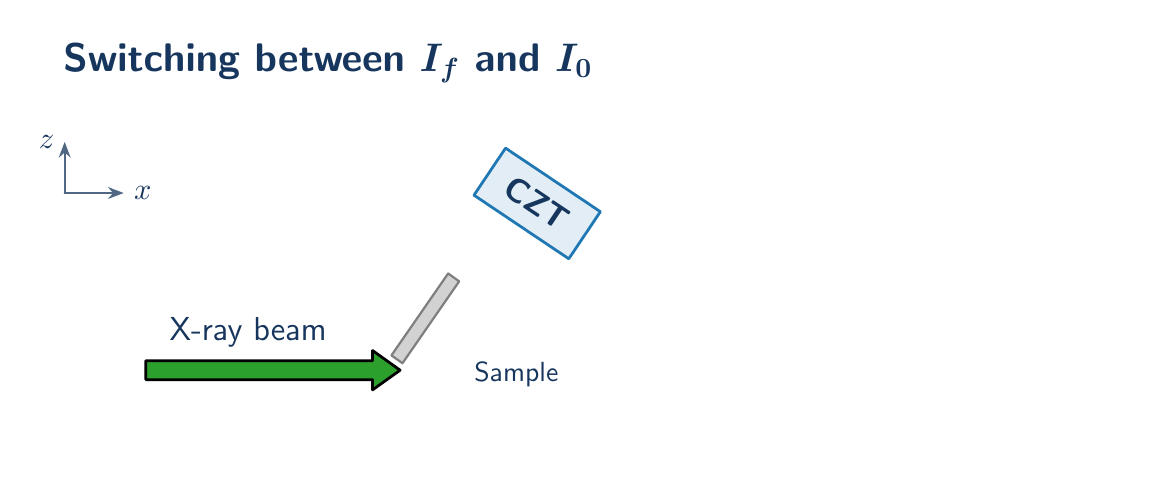
\begin{tikzpicture}[x=1cm,y=1cm,line join=round,line cap=round,
 every node/.style={font=\sffamily\fontsize{12}{14}\selectfont,text=ink},
]
\newcommand{\BeamArrow}[4]{%
  \begin{scope}
    \coordinate (beamStart) at #3;
    \coordinate (beamEnd) at #4;
    \path let \p1 = ($(beamEnd)-(beamStart)$),
      \n1 = {atan2(\y1,\x1)}, \n2 = {veclen(\x1,\y1)} in
      \pgfextra{\xdef\beamAngle{\n1}\xdef\beamLength{\n2}};
    \begin{scope}[shift={(beamStart)},rotate=\beamAngle]
      \path[fill=#1,draw=black,opacity=#2,line width=.35mm,line join=round]
        (0,-1.2mm) -- (\beamLength-3.5mm,-1.2mm)
        -- (\beamLength-3.5mm,-2.5mm) -- (\beamLength,0)
        -- (\beamLength-3.5mm,2.5mm) -- (\beamLength-3.5mm,1.2mm)
        -- (0,1.2mm) -- cycle;
    \end{scope}
  \end{scope}
}
\path[use as bounding box] (-1.05,-1.25) rectangle (12.8878,4.35);
\node[anchor=west,font=\sffamily\bfseries\fontsize{14}{17}\selectfont] at (-.72,3.9) {Switching between $\bm{I_f}$ and $\bm{I_0}$};
\draw[ink!75,line width=.8pt,-{Stealth[length=2mm]}] (-.58,2.25) -- (.17,2.25) node[anchor=west,font=\sffamily\fontsize{11}{13}\selectfont] {$x$};
\draw[ink!75,line width=.8pt,-{Stealth[length=2mm]}] (-.58,2.25) -- (-.58,2.9) node[anchor=east,font=\sffamily\fontsize{11}{13}\selectfont] {$z$};
\BeamArrow{beamgreen}{1.0000}{(.45,0)}{(3.68,0)}
\node at (1.75,.48) {X-ray beam};
\BeamArrow{beamgreen}{0.0000}{(.45,0)}{(5.98,0)}
\BeamArrow{fluororange}{0.0003}{(4,.35)}{(4,2.03)}
\node[opacity=0.0003,anchor=west] at (4.35,1.25) {$\bm{I_f}$};
\node[opacity=0.0000] at (5.25,.48) {$\bm{I_0}$};
\begin{scope}[shift={(4,0.6583)}]
\path[draw=samplegray,fill=samplegray!35,line width=.8pt] (-.43,-.47) -- (-.29,-.57) -- (.43,.47) -- (.29,.57) -- cycle;
\end{scope}
\node[anchor=west,font=\sffamily\fontsize{10}{12}\selectfont] at (4.5,-0.0617) {Sample};
\begin{scope}[shift={(5.4206,2.1177)},rotate=-33.8542,transform shape]
\node[draw=detectorblue,fill=detectorblue!13,line width=1pt,minimum width=1.45cm,minimum height=.72cm,inner sep=2pt,font=\sffamily\bfseries\fontsize{13}{15}\selectfont] {CZT};
\end{scope}
\node[opacity=0.0003,font=\sffamily\bfseries\fontsize{13}{15}\selectfont,text=motioncyan] at (9.4,2.2) {Fluorescence};
\node[opacity=0.0000,font=\sffamily\bfseries\fontsize{13}{15}\selectfont,text=motioncyan] at (9.4,2.2) {Incident beam};
\end{tikzpicture}
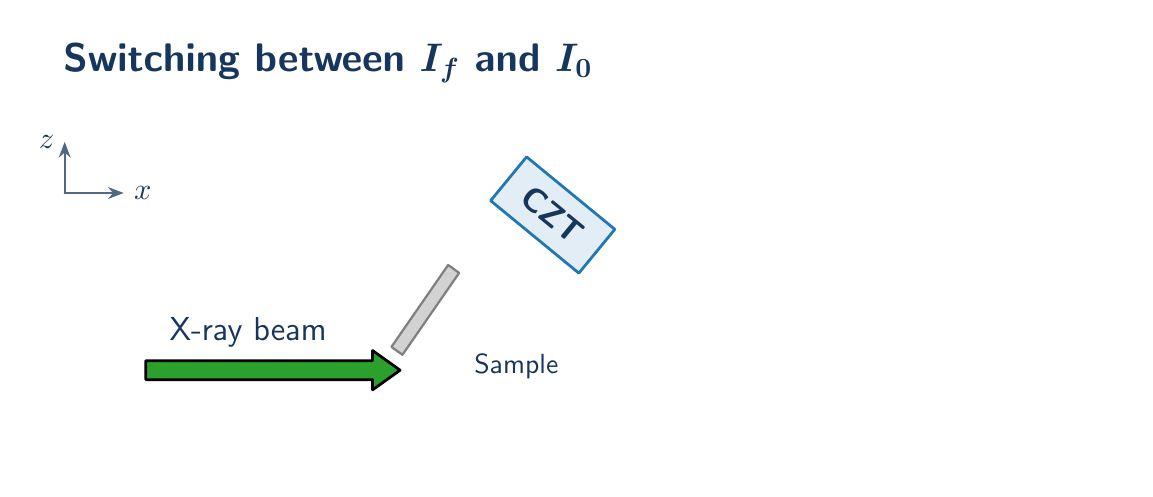
\begin{tikzpicture}[x=1cm,y=1cm,line join=round,line cap=round,
 every node/.style={font=\sffamily\fontsize{12}{14}\selectfont,text=ink},
]
\newcommand{\BeamArrow}[4]{%
  \begin{scope}
    \coordinate (beamStart) at #3;
    \coordinate (beamEnd) at #4;
    \path let \p1 = ($(beamEnd)-(beamStart)$),
      \n1 = {atan2(\y1,\x1)}, \n2 = {veclen(\x1,\y1)} in
      \pgfextra{\xdef\beamAngle{\n1}\xdef\beamLength{\n2}};
    \begin{scope}[shift={(beamStart)},rotate=\beamAngle]
      \path[fill=#1,draw=black,opacity=#2,line width=.35mm,line join=round]
        (0,-1.2mm) -- (\beamLength-3.5mm,-1.2mm)
        -- (\beamLength-3.5mm,-2.5mm) -- (\beamLength,0)
        -- (\beamLength-3.5mm,2.5mm) -- (\beamLength-3.5mm,1.2mm)
        -- (0,1.2mm) -- cycle;
    \end{scope}
  \end{scope}
}
\path[use as bounding box] (-1.05,-1.25) rectangle (12.8878,4.35);
\node[anchor=west,font=\sffamily\bfseries\fontsize{14}{17}\selectfont] at (-.72,3.9) {Switching between $\bm{I_f}$ and $\bm{I_0}$};
\draw[ink!75,line width=.8pt,-{Stealth[length=2mm]}] (-.58,2.25) -- (.17,2.25) node[anchor=west,font=\sffamily\fontsize{11}{13}\selectfont] {$x$};
\draw[ink!75,line width=.8pt,-{Stealth[length=2mm]}] (-.58,2.25) -- (-.58,2.9) node[anchor=east,font=\sffamily\fontsize{11}{13}\selectfont] {$z$};
\BeamArrow{beamgreen}{1.0000}{(.45,0)}{(3.68,0)}
\node at (1.75,.48) {X-ray beam};
\BeamArrow{beamgreen}{0.0000}{(.45,0)}{(5.98,0)}
\BeamArrow{fluororange}{0.0000}{(4,.35)}{(4,2.03)}
\node[opacity=0.0000,anchor=west] at (4.35,1.25) {$\bm{I_f}$};
\node[opacity=0.0000] at (5.25,.48) {$\bm{I_0}$};
\begin{scope}[shift={(4,0.7659)}]
\path[draw=samplegray,fill=samplegray!35,line width=.8pt] (-.43,-.47) -- (-.29,-.57) -- (.43,.47) -- (.29,.57) -- cycle;
\end{scope}
\node[anchor=west,font=\sffamily\fontsize{10}{12}\selectfont] at (4.5,0.0459) {Sample};
\begin{scope}[shift={(5.6182,1.9708)},rotate=-39.3880,transform shape]
\node[draw=detectorblue,fill=detectorblue!13,line width=1pt,minimum width=1.45cm,minimum height=.72cm,inner sep=2pt,font=\sffamily\bfseries\fontsize{13}{15}\selectfont] {CZT};
\end{scope}
\node[opacity=0.0000,font=\sffamily\bfseries\fontsize{13}{15}\selectfont,text=motioncyan] at (9.4,2.2) {Fluorescence};
\node[opacity=0.0000,font=\sffamily\bfseries\fontsize{13}{15}\selectfont,text=motioncyan] at (9.4,2.2) {Incident beam};
\end{tikzpicture}
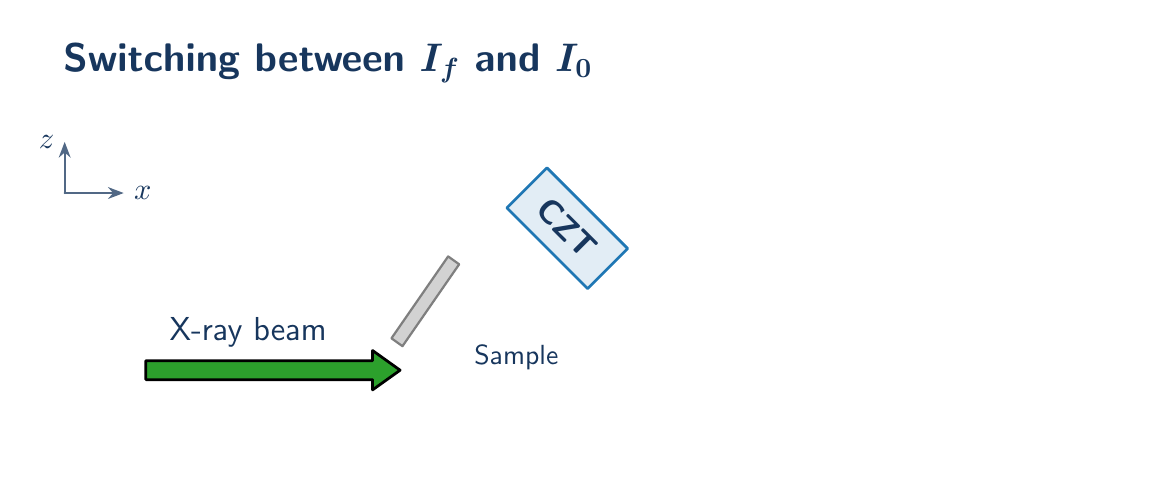
\begin{tikzpicture}[x=1cm,y=1cm,line join=round,line cap=round,
 every node/.style={font=\sffamily\fontsize{12}{14}\selectfont,text=ink},
]
\newcommand{\BeamArrow}[4]{%
  \begin{scope}
    \coordinate (beamStart) at #3;
    \coordinate (beamEnd) at #4;
    \path let \p1 = ($(beamEnd)-(beamStart)$),
      \n1 = {atan2(\y1,\x1)}, \n2 = {veclen(\x1,\y1)} in
      \pgfextra{\xdef\beamAngle{\n1}\xdef\beamLength{\n2}};
    \begin{scope}[shift={(beamStart)},rotate=\beamAngle]
      \path[fill=#1,draw=black,opacity=#2,line width=.35mm,line join=round]
        (0,-1.2mm) -- (\beamLength-3.5mm,-1.2mm)
        -- (\beamLength-3.5mm,-2.5mm) -- (\beamLength,0)
        -- (\beamLength-3.5mm,2.5mm) -- (\beamLength-3.5mm,1.2mm)
        -- (0,1.2mm) -- cycle;
    \end{scope}
  \end{scope}
}
\path[use as bounding box] (-1.05,-1.25) rectangle (12.8878,4.35);
\node[anchor=west,font=\sffamily\bfseries\fontsize{14}{17}\selectfont] at (-.72,3.9) {Switching between $\bm{I_f}$ and $\bm{I_0}$};
\draw[ink!75,line width=.8pt,-{Stealth[length=2mm]}] (-.58,2.25) -- (.17,2.25) node[anchor=west,font=\sffamily\fontsize{11}{13}\selectfont] {$x$};
\draw[ink!75,line width=.8pt,-{Stealth[length=2mm]}] (-.58,2.25) -- (-.58,2.9) node[anchor=east,font=\sffamily\fontsize{11}{13}\selectfont] {$z$};
\BeamArrow{beamgreen}{1.0000}{(.45,0)}{(3.68,0)}
\node at (1.75,.48) {X-ray beam};
\BeamArrow{beamgreen}{0.0000}{(.45,0)}{(5.98,0)}
\BeamArrow{fluororange}{0.0000}{(4,.35)}{(4,2.03)}
\node[opacity=0.0000,anchor=west] at (4.35,1.25) {$\bm{I_f}$};
\node[opacity=0.0000] at (5.25,.48) {$\bm{I_0}$};
\begin{scope}[shift={(4,0.8750)}]
\path[draw=samplegray,fill=samplegray!35,line width=.8pt] (-.43,-.47) -- (-.29,-.57) -- (.43,.47) -- (.29,.57) -- cycle;
\end{scope}
\node[anchor=west,font=\sffamily\fontsize{10}{12}\selectfont] at (4.5,0.1550) {Sample};
\begin{scope}[shift={(5.8031,1.8031)},rotate=-45.0000,transform shape]
\node[draw=detectorblue,fill=detectorblue!13,line width=1pt,minimum width=1.45cm,minimum height=.72cm,inner sep=2pt,font=\sffamily\bfseries\fontsize{13}{15}\selectfont] {CZT};
\end{scope}
\node[opacity=0.0000,font=\sffamily\bfseries\fontsize{13}{15}\selectfont,text=motioncyan] at (9.4,2.2) {Fluorescence};
\node[opacity=0.0000,font=\sffamily\bfseries\fontsize{13}{15}\selectfont,text=motioncyan] at (9.4,2.2) {Incident beam};
\end{tikzpicture}
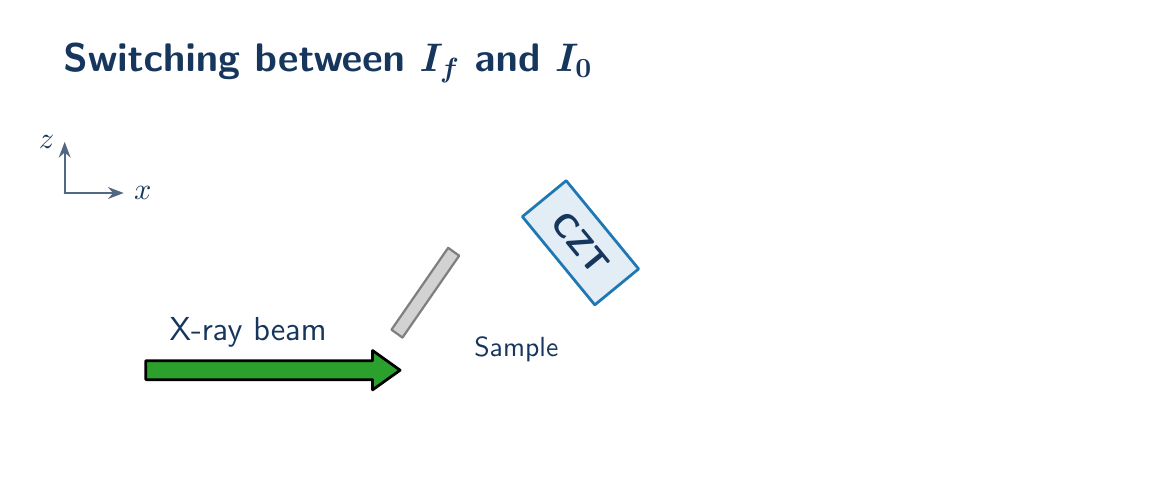
\begin{tikzpicture}[x=1cm,y=1cm,line join=round,line cap=round,
 every node/.style={font=\sffamily\fontsize{12}{14}\selectfont,text=ink},
]
\newcommand{\BeamArrow}[4]{%
  \begin{scope}
    \coordinate (beamStart) at #3;
    \coordinate (beamEnd) at #4;
    \path let \p1 = ($(beamEnd)-(beamStart)$),
      \n1 = {atan2(\y1,\x1)}, \n2 = {veclen(\x1,\y1)} in
      \pgfextra{\xdef\beamAngle{\n1}\xdef\beamLength{\n2}};
    \begin{scope}[shift={(beamStart)},rotate=\beamAngle]
      \path[fill=#1,draw=black,opacity=#2,line width=.35mm,line join=round]
        (0,-1.2mm) -- (\beamLength-3.5mm,-1.2mm)
        -- (\beamLength-3.5mm,-2.5mm) -- (\beamLength,0)
        -- (\beamLength-3.5mm,2.5mm) -- (\beamLength-3.5mm,1.2mm)
        -- (0,1.2mm) -- cycle;
    \end{scope}
  \end{scope}
}
\path[use as bounding box] (-1.05,-1.25) rectangle (12.8878,4.35);
\node[anchor=west,font=\sffamily\bfseries\fontsize{14}{17}\selectfont] at (-.72,3.9) {Switching between $\bm{I_f}$ and $\bm{I_0}$};
\draw[ink!75,line width=.8pt,-{Stealth[length=2mm]}] (-.58,2.25) -- (.17,2.25) node[anchor=west,font=\sffamily\fontsize{11}{13}\selectfont] {$x$};
\draw[ink!75,line width=.8pt,-{Stealth[length=2mm]}] (-.58,2.25) -- (-.58,2.9) node[anchor=east,font=\sffamily\fontsize{11}{13}\selectfont] {$z$};
\BeamArrow{beamgreen}{1.0000}{(.45,0)}{(3.68,0)}
\node at (1.75,.48) {X-ray beam};
\BeamArrow{beamgreen}{0.0000}{(.45,0)}{(5.98,0)}
\BeamArrow{fluororange}{0.0000}{(4,.35)}{(4,2.03)}
\node[opacity=0.0000,anchor=west] at (4.35,1.25) {$\bm{I_f}$};
\node[opacity=0.0000] at (5.25,.48) {$\bm{I_0}$};
\begin{scope}[shift={(4,0.9841)}]
\path[draw=samplegray,fill=samplegray!35,line width=.8pt] (-.43,-.47) -- (-.29,-.57) -- (.43,.47) -- (.29,.57) -- cycle;
\end{scope}
\node[anchor=west,font=\sffamily\fontsize{10}{12}\selectfont] at (4.5,0.2641) {Sample};
\begin{scope}[shift={(5.9708,1.6182)},rotate=-50.6120,transform shape]
\node[draw=detectorblue,fill=detectorblue!13,line width=1pt,minimum width=1.45cm,minimum height=.72cm,inner sep=2pt,font=\sffamily\bfseries\fontsize{13}{15}\selectfont] {CZT};
\end{scope}
\node[opacity=0.0000,font=\sffamily\bfseries\fontsize{13}{15}\selectfont,text=motioncyan] at (9.4,2.2) {Fluorescence};
\node[opacity=0.0000,font=\sffamily\bfseries\fontsize{13}{15}\selectfont,text=motioncyan] at (9.4,2.2) {Incident beam};
\end{tikzpicture}
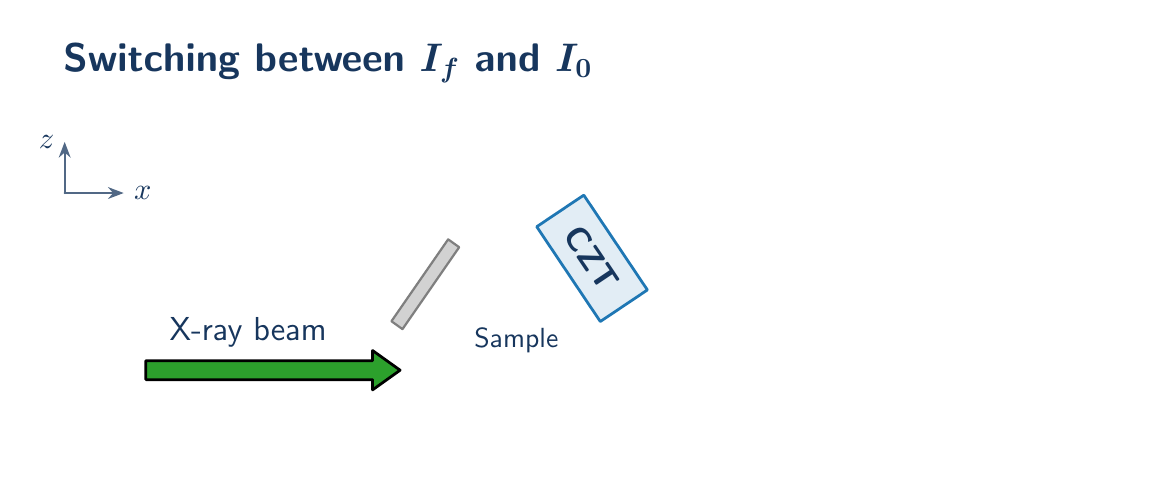
\begin{tikzpicture}[x=1cm,y=1cm,line join=round,line cap=round,
 every node/.style={font=\sffamily\fontsize{12}{14}\selectfont,text=ink},
]
\newcommand{\BeamArrow}[4]{%
  \begin{scope}
    \coordinate (beamStart) at #3;
    \coordinate (beamEnd) at #4;
    \path let \p1 = ($(beamEnd)-(beamStart)$),
      \n1 = {atan2(\y1,\x1)}, \n2 = {veclen(\x1,\y1)} in
      \pgfextra{\xdef\beamAngle{\n1}\xdef\beamLength{\n2}};
    \begin{scope}[shift={(beamStart)},rotate=\beamAngle]
      \path[fill=#1,draw=black,opacity=#2,line width=.35mm,line join=round]
        (0,-1.2mm) -- (\beamLength-3.5mm,-1.2mm)
        -- (\beamLength-3.5mm,-2.5mm) -- (\beamLength,0)
        -- (\beamLength-3.5mm,2.5mm) -- (\beamLength-3.5mm,1.2mm)
        -- (0,1.2mm) -- cycle;
    \end{scope}
  \end{scope}
}
\path[use as bounding box] (-1.05,-1.25) rectangle (12.8878,4.35);
\node[anchor=west,font=\sffamily\bfseries\fontsize{14}{17}\selectfont] at (-.72,3.9) {Switching between $\bm{I_f}$ and $\bm{I_0}$};
\draw[ink!75,line width=.8pt,-{Stealth[length=2mm]}] (-.58,2.25) -- (.17,2.25) node[anchor=west,font=\sffamily\fontsize{11}{13}\selectfont] {$x$};
\draw[ink!75,line width=.8pt,-{Stealth[length=2mm]}] (-.58,2.25) -- (-.58,2.9) node[anchor=east,font=\sffamily\fontsize{11}{13}\selectfont] {$z$};
\BeamArrow{beamgreen}{0.9997}{(.45,0)}{(3.68,0)}
\node at (1.75,.48) {X-ray beam};
\BeamArrow{beamgreen}{0.0003}{(.45,0)}{(5.98,0)}
\BeamArrow{fluororange}{0.0000}{(4,.35)}{(4,2.03)}
\node[opacity=0.0000,anchor=west] at (4.35,1.25) {$\bm{I_f}$};
\node[opacity=0.0003] at (5.25,.48) {$\bm{I_0}$};
\begin{scope}[shift={(4,1.0917)}]
\path[draw=samplegray,fill=samplegray!35,line width=.8pt] (-.43,-.47) -- (-.29,-.57) -- (.43,.47) -- (.29,.57) -- cycle;
\end{scope}
\node[anchor=west,font=\sffamily\fontsize{10}{12}\selectfont] at (4.5,0.3717) {Sample};
\begin{scope}[shift={(6.1177,1.4206)},rotate=-56.1458,transform shape]
\node[draw=detectorblue,fill=detectorblue!13,line width=1pt,minimum width=1.45cm,minimum height=.72cm,inner sep=2pt,font=\sffamily\bfseries\fontsize{13}{15}\selectfont] {CZT};
\end{scope}
\node[opacity=0.0000,font=\sffamily\bfseries\fontsize{13}{15}\selectfont,text=motioncyan] at (9.4,2.2) {Fluorescence};
\node[opacity=0.0003,font=\sffamily\bfseries\fontsize{13}{15}\selectfont,text=motioncyan] at (9.4,2.2) {Incident beam};
\end{tikzpicture}
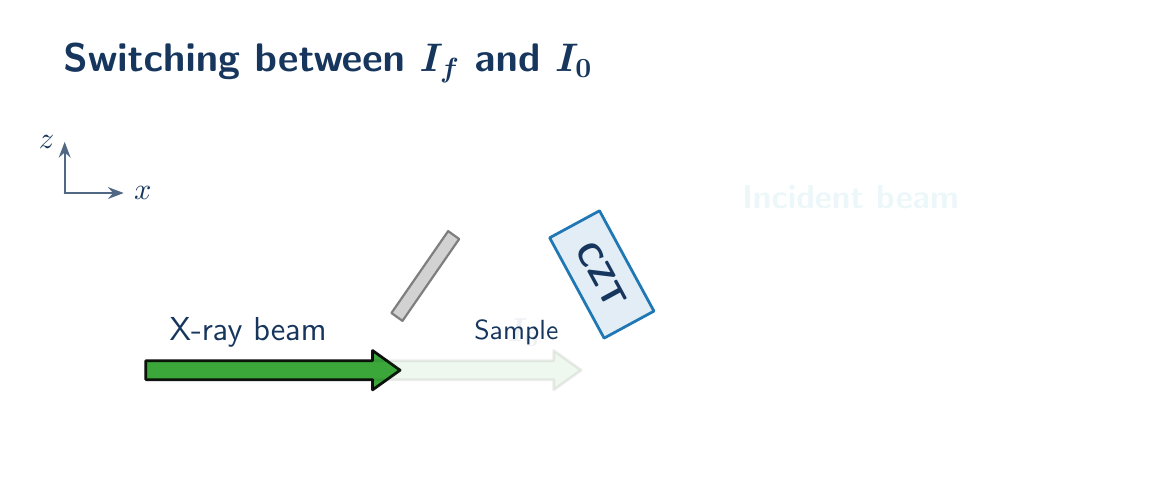
\begin{tikzpicture}[x=1cm,y=1cm,line join=round,line cap=round,
 every node/.style={font=\sffamily\fontsize{12}{14}\selectfont,text=ink},
]
\newcommand{\BeamArrow}[4]{%
  \begin{scope}
    \coordinate (beamStart) at #3;
    \coordinate (beamEnd) at #4;
    \path let \p1 = ($(beamEnd)-(beamStart)$),
      \n1 = {atan2(\y1,\x1)}, \n2 = {veclen(\x1,\y1)} in
      \pgfextra{\xdef\beamAngle{\n1}\xdef\beamLength{\n2}};
    \begin{scope}[shift={(beamStart)},rotate=\beamAngle]
      \path[fill=#1,draw=black,opacity=#2,line width=.35mm,line join=round]
        (0,-1.2mm) -- (\beamLength-3.5mm,-1.2mm)
        -- (\beamLength-3.5mm,-2.5mm) -- (\beamLength,0)
        -- (\beamLength-3.5mm,2.5mm) -- (\beamLength-3.5mm,1.2mm)
        -- (0,1.2mm) -- cycle;
    \end{scope}
  \end{scope}
}
\path[use as bounding box] (-1.05,-1.25) rectangle (12.8878,4.35);
\node[anchor=west,font=\sffamily\bfseries\fontsize{14}{17}\selectfont] at (-.72,3.9) {Switching between $\bm{I_f}$ and $\bm{I_0}$};
\draw[ink!75,line width=.8pt,-{Stealth[length=2mm]}] (-.58,2.25) -- (.17,2.25) node[anchor=west,font=\sffamily\fontsize{11}{13}\selectfont] {$x$};
\draw[ink!75,line width=.8pt,-{Stealth[length=2mm]}] (-.58,2.25) -- (-.58,2.9) node[anchor=east,font=\sffamily\fontsize{11}{13}\selectfont] {$z$};
\BeamArrow{beamgreen}{0.9254}{(.45,0)}{(3.68,0)}
\node at (1.75,.48) {X-ray beam};
\BeamArrow{beamgreen}{0.0746}{(.45,0)}{(5.98,0)}
\BeamArrow{fluororange}{0.0000}{(4,.35)}{(4,2.03)}
\node[opacity=0.0000,anchor=west] at (4.35,1.25) {$\bm{I_f}$};
\node[opacity=0.0746] at (5.25,.48) {$\bm{I_0}$};
\begin{scope}[shift={(4,1.1963)}]
\path[draw=samplegray,fill=samplegray!35,line width=.8pt] (-.43,-.47) -- (-.29,-.57) -- (.43,.47) -- (.29,.57) -- cycle;
\end{scope}
\node[anchor=west,font=\sffamily\fontsize{10}{12}\selectfont] at (4.5,0.4763) {Sample};
\begin{scope}[shift={(6.2415,1.2158)},rotate=-61.5234,transform shape]
\node[draw=detectorblue,fill=detectorblue!13,line width=1pt,minimum width=1.45cm,minimum height=.72cm,inner sep=2pt,font=\sffamily\bfseries\fontsize{13}{15}\selectfont] {CZT};
\end{scope}
\node[opacity=0.0000,font=\sffamily\bfseries\fontsize{13}{15}\selectfont,text=motioncyan] at (9.4,2.2) {Fluorescence};
\node[opacity=0.0746,font=\sffamily\bfseries\fontsize{13}{15}\selectfont,text=motioncyan] at (9.4,2.2) {Incident beam};
\end{tikzpicture}
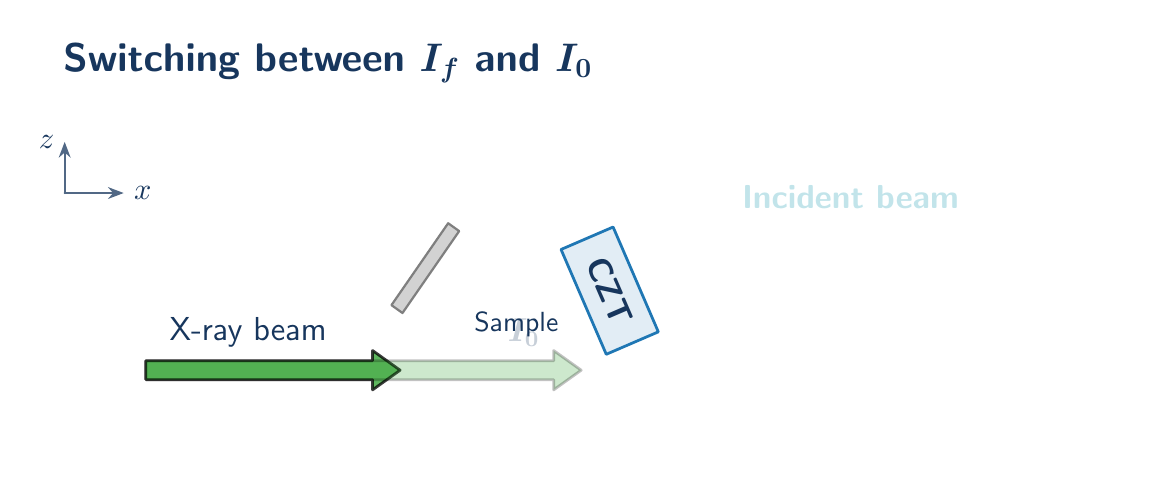
\begin{tikzpicture}[x=1cm,y=1cm,line join=round,line cap=round,
 every node/.style={font=\sffamily\fontsize{12}{14}\selectfont,text=ink},
]
\newcommand{\BeamArrow}[4]{%
  \begin{scope}
    \coordinate (beamStart) at #3;
    \coordinate (beamEnd) at #4;
    \path let \p1 = ($(beamEnd)-(beamStart)$),
      \n1 = {atan2(\y1,\x1)}, \n2 = {veclen(\x1,\y1)} in
      \pgfextra{\xdef\beamAngle{\n1}\xdef\beamLength{\n2}};
    \begin{scope}[shift={(beamStart)},rotate=\beamAngle]
      \path[fill=#1,draw=black,opacity=#2,line width=.35mm,line join=round]
        (0,-1.2mm) -- (\beamLength-3.5mm,-1.2mm)
        -- (\beamLength-3.5mm,-2.5mm) -- (\beamLength,0)
        -- (\beamLength-3.5mm,2.5mm) -- (\beamLength-3.5mm,1.2mm)
        -- (0,1.2mm) -- cycle;
    \end{scope}
  \end{scope}
}
\path[use as bounding box] (-1.05,-1.25) rectangle (12.8878,4.35);
\node[anchor=west,font=\sffamily\bfseries\fontsize{14}{17}\selectfont] at (-.72,3.9) {Switching between $\bm{I_f}$ and $\bm{I_0}$};
\draw[ink!75,line width=.8pt,-{Stealth[length=2mm]}] (-.58,2.25) -- (.17,2.25) node[anchor=west,font=\sffamily\fontsize{11}{13}\selectfont] {$x$};
\draw[ink!75,line width=.8pt,-{Stealth[length=2mm]}] (-.58,2.25) -- (-.58,2.9) node[anchor=east,font=\sffamily\fontsize{11}{13}\selectfont] {$z$};
\BeamArrow{beamgreen}{0.7613}{(.45,0)}{(3.68,0)}
\node at (1.75,.48) {X-ray beam};
\BeamArrow{beamgreen}{0.2387}{(.45,0)}{(5.98,0)}
\BeamArrow{fluororange}{0.0000}{(4,.35)}{(4,2.03)}
\node[opacity=0.0000,anchor=west] at (4.35,1.25) {$\bm{I_f}$};
\node[opacity=0.2387] at (5.25,.48) {$\bm{I_0}$};
\begin{scope}[shift={(4,1.2963)}]
\path[draw=samplegray,fill=samplegray!35,line width=.8pt] (-.43,-.47) -- (-.29,-.57) -- (.43,.47) -- (.29,.57) -- cycle;
\end{scope}
\node[anchor=west,font=\sffamily\fontsize{10}{12}\selectfont] at (4.5,0.5763) {Sample};
\begin{scope}[shift={(6.3415,1.0100)},rotate=-66.6667,transform shape]
\node[draw=detectorblue,fill=detectorblue!13,line width=1pt,minimum width=1.45cm,minimum height=.72cm,inner sep=2pt,font=\sffamily\bfseries\fontsize{13}{15}\selectfont] {CZT};
\end{scope}
\node[opacity=0.0000,font=\sffamily\bfseries\fontsize{13}{15}\selectfont,text=motioncyan] at (9.4,2.2) {Fluorescence};
\node[opacity=0.2387,font=\sffamily\bfseries\fontsize{13}{15}\selectfont,text=motioncyan] at (9.4,2.2) {Incident beam};
\end{tikzpicture}
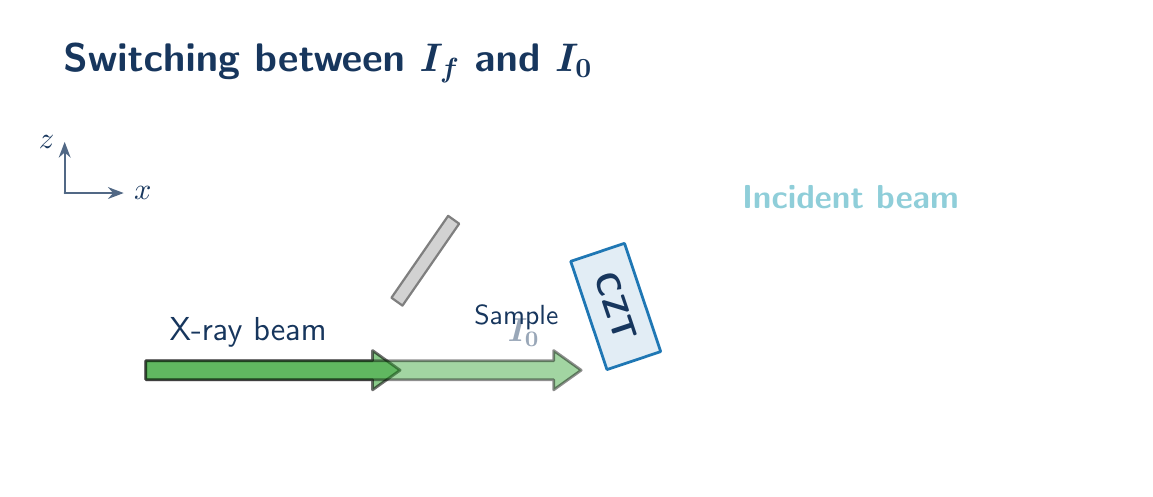
\begin{tikzpicture}[x=1cm,y=1cm,line join=round,line cap=round,
 every node/.style={font=\sffamily\fontsize{12}{14}\selectfont,text=ink},
]
\newcommand{\BeamArrow}[4]{%
  \begin{scope}
    \coordinate (beamStart) at #3;
    \coordinate (beamEnd) at #4;
    \path let \p1 = ($(beamEnd)-(beamStart)$),
      \n1 = {atan2(\y1,\x1)}, \n2 = {veclen(\x1,\y1)} in
      \pgfextra{\xdef\beamAngle{\n1}\xdef\beamLength{\n2}};
    \begin{scope}[shift={(beamStart)},rotate=\beamAngle]
      \path[fill=#1,draw=black,opacity=#2,line width=.35mm,line join=round]
        (0,-1.2mm) -- (\beamLength-3.5mm,-1.2mm)
        -- (\beamLength-3.5mm,-2.5mm) -- (\beamLength,0)
        -- (\beamLength-3.5mm,2.5mm) -- (\beamLength-3.5mm,1.2mm)
        -- (0,1.2mm) -- cycle;
    \end{scope}
  \end{scope}
}
\path[use as bounding box] (-1.05,-1.25) rectangle (12.8878,4.35);
\node[anchor=west,font=\sffamily\bfseries\fontsize{14}{17}\selectfont] at (-.72,3.9) {Switching between $\bm{I_f}$ and $\bm{I_0}$};
\draw[ink!75,line width=.8pt,-{Stealth[length=2mm]}] (-.58,2.25) -- (.17,2.25) node[anchor=west,font=\sffamily\fontsize{11}{13}\selectfont] {$x$};
\draw[ink!75,line width=.8pt,-{Stealth[length=2mm]}] (-.58,2.25) -- (-.58,2.9) node[anchor=east,font=\sffamily\fontsize{11}{13}\selectfont] {$z$};
\BeamArrow{beamgreen}{0.5614}{(.45,0)}{(3.68,0)}
\node at (1.75,.48) {X-ray beam};
\BeamArrow{beamgreen}{0.4386}{(.45,0)}{(5.98,0)}
\BeamArrow{fluororange}{0.0000}{(4,.35)}{(4,2.03)}
\node[opacity=0.0000,anchor=west] at (4.35,1.25) {$\bm{I_f}$};
\node[opacity=0.4386] at (5.25,.48) {$\bm{I_0}$};
\begin{scope}[shift={(4,1.3902)}]
\path[draw=samplegray,fill=samplegray!35,line width=.8pt] (-.43,-.47) -- (-.29,-.57) -- (.43,.47) -- (.29,.57) -- cycle;
\end{scope}
\node[anchor=west,font=\sffamily\fontsize{10}{12}\selectfont] at (4.5,0.6702) {Sample};
\begin{scope}[shift={(6.4182,0.8092)},rotate=-71.4974,transform shape]
\node[draw=detectorblue,fill=detectorblue!13,line width=1pt,minimum width=1.45cm,minimum height=.72cm,inner sep=2pt,font=\sffamily\bfseries\fontsize{13}{15}\selectfont] {CZT};
\end{scope}
\node[opacity=0.0000,font=\sffamily\bfseries\fontsize{13}{15}\selectfont,text=motioncyan] at (9.4,2.2) {Fluorescence};
\node[opacity=0.4386,font=\sffamily\bfseries\fontsize{13}{15}\selectfont,text=motioncyan] at (9.4,2.2) {Incident beam};
\end{tikzpicture}
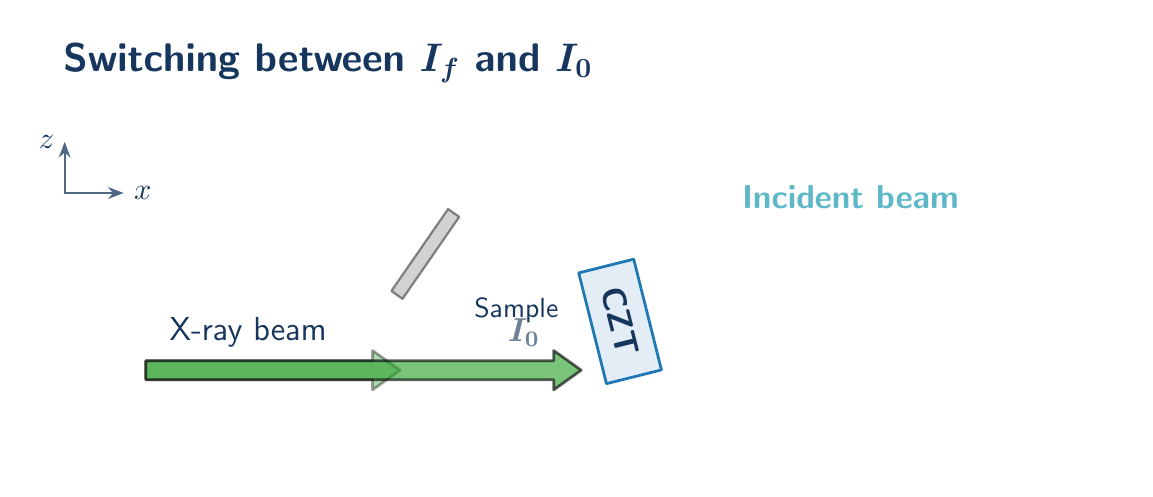
\begin{tikzpicture}[x=1cm,y=1cm,line join=round,line cap=round,
 every node/.style={font=\sffamily\fontsize{12}{14}\selectfont,text=ink},
]
\newcommand{\BeamArrow}[4]{%
  \begin{scope}
    \coordinate (beamStart) at #3;
    \coordinate (beamEnd) at #4;
    \path let \p1 = ($(beamEnd)-(beamStart)$),
      \n1 = {atan2(\y1,\x1)}, \n2 = {veclen(\x1,\y1)} in
      \pgfextra{\xdef\beamAngle{\n1}\xdef\beamLength{\n2}};
    \begin{scope}[shift={(beamStart)},rotate=\beamAngle]
      \path[fill=#1,draw=black,opacity=#2,line width=.35mm,line join=round]
        (0,-1.2mm) -- (\beamLength-3.5mm,-1.2mm)
        -- (\beamLength-3.5mm,-2.5mm) -- (\beamLength,0)
        -- (\beamLength-3.5mm,2.5mm) -- (\beamLength-3.5mm,1.2mm)
        -- (0,1.2mm) -- cycle;
    \end{scope}
  \end{scope}
}
\path[use as bounding box] (-1.05,-1.25) rectangle (12.8878,4.35);
\node[anchor=west,font=\sffamily\bfseries\fontsize{14}{17}\selectfont] at (-.72,3.9) {Switching between $\bm{I_f}$ and $\bm{I_0}$};
\draw[ink!75,line width=.8pt,-{Stealth[length=2mm]}] (-.58,2.25) -- (.17,2.25) node[anchor=west,font=\sffamily\fontsize{11}{13}\selectfont] {$x$};
\draw[ink!75,line width=.8pt,-{Stealth[length=2mm]}] (-.58,2.25) -- (-.58,2.9) node[anchor=east,font=\sffamily\fontsize{11}{13}\selectfont] {$z$};
\BeamArrow{beamgreen}{0.3682}{(.45,0)}{(3.68,0)}
\node at (1.75,.48) {X-ray beam};
\BeamArrow{beamgreen}{0.6318}{(.45,0)}{(5.98,0)}
\BeamArrow{fluororange}{0.0000}{(4,.35)}{(4,2.03)}
\node[opacity=0.0000,anchor=west] at (4.35,1.25) {$\bm{I_f}$};
\node[opacity=0.6318] at (5.25,.48) {$\bm{I_0}$};
\begin{scope}[shift={(4,1.4766)}]
\path[draw=samplegray,fill=samplegray!35,line width=.8pt] (-.43,-.47) -- (-.29,-.57) -- (.43,.47) -- (.29,.57) -- cycle;
\end{scope}
\node[anchor=west,font=\sffamily\fontsize{10}{12}\selectfont] at (4.5,0.7566) {Sample};
\begin{scope}[shift={(6.4736,0.6196)},rotate=-75.9375,transform shape]
\node[draw=detectorblue,fill=detectorblue!13,line width=1pt,minimum width=1.45cm,minimum height=.72cm,inner sep=2pt,font=\sffamily\bfseries\fontsize{13}{15}\selectfont] {CZT};
\end{scope}
\node[opacity=0.0000,font=\sffamily\bfseries\fontsize{13}{15}\selectfont,text=motioncyan] at (9.4,2.2) {Fluorescence};
\node[opacity=0.6318,font=\sffamily\bfseries\fontsize{13}{15}\selectfont,text=motioncyan] at (9.4,2.2) {Incident beam};
\end{tikzpicture}
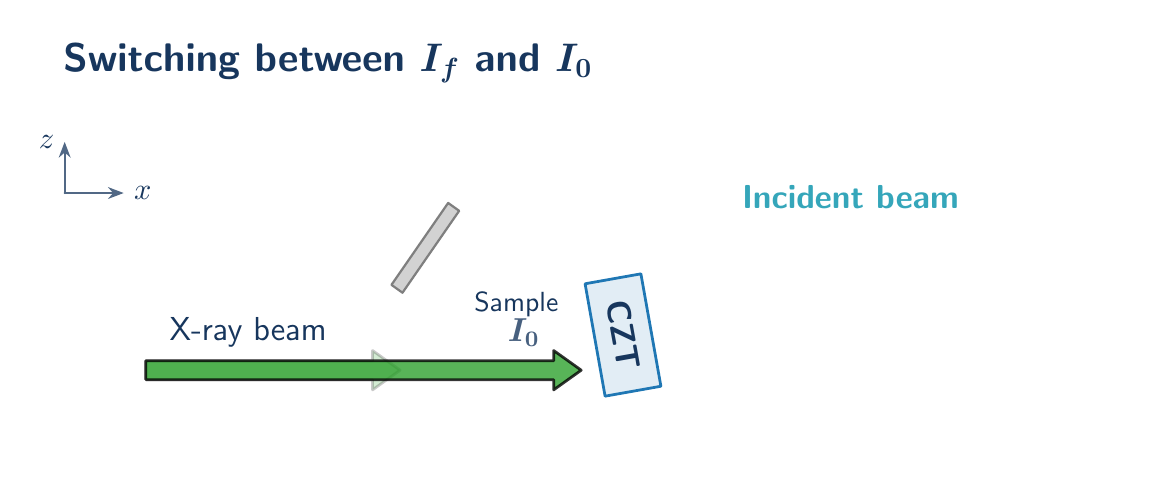
\begin{tikzpicture}[x=1cm,y=1cm,line join=round,line cap=round,
 every node/.style={font=\sffamily\fontsize{12}{14}\selectfont,text=ink},
]
\newcommand{\BeamArrow}[4]{%
  \begin{scope}
    \coordinate (beamStart) at #3;
    \coordinate (beamEnd) at #4;
    \path let \p1 = ($(beamEnd)-(beamStart)$),
      \n1 = {atan2(\y1,\x1)}, \n2 = {veclen(\x1,\y1)} in
      \pgfextra{\xdef\beamAngle{\n1}\xdef\beamLength{\n2}};
    \begin{scope}[shift={(beamStart)},rotate=\beamAngle]
      \path[fill=#1,draw=black,opacity=#2,line width=.35mm,line join=round]
        (0,-1.2mm) -- (\beamLength-3.5mm,-1.2mm)
        -- (\beamLength-3.5mm,-2.5mm) -- (\beamLength,0)
        -- (\beamLength-3.5mm,2.5mm) -- (\beamLength-3.5mm,1.2mm)
        -- (0,1.2mm) -- cycle;
    \end{scope}
  \end{scope}
}
\path[use as bounding box] (-1.05,-1.25) rectangle (12.8878,4.35);
\node[anchor=west,font=\sffamily\bfseries\fontsize{14}{17}\selectfont] at (-.72,3.9) {Switching between $\bm{I_f}$ and $\bm{I_0}$};
\draw[ink!75,line width=.8pt,-{Stealth[length=2mm]}] (-.58,2.25) -- (.17,2.25) node[anchor=west,font=\sffamily\fontsize{11}{13}\selectfont] {$x$};
\draw[ink!75,line width=.8pt,-{Stealth[length=2mm]}] (-.58,2.25) -- (-.58,2.9) node[anchor=east,font=\sffamily\fontsize{11}{13}\selectfont] {$z$};
\BeamArrow{beamgreen}{0.2098}{(.45,0)}{(3.68,0)}
\node at (1.75,.48) {X-ray beam};
\BeamArrow{beamgreen}{0.7902}{(.45,0)}{(5.98,0)}
\BeamArrow{fluororange}{0.0000}{(4,.35)}{(4,2.03)}
\node[opacity=0.0000,anchor=west] at (4.35,1.25) {$\bm{I_f}$};
\node[opacity=0.7902] at (5.25,.48) {$\bm{I_0}$};
\begin{scope}[shift={(4,1.5538)}]
\path[draw=samplegray,fill=samplegray!35,line width=.8pt] (-.43,-.47) -- (-.29,-.57) -- (.43,.47) -- (.29,.57) -- cycle;
\end{scope}
\node[anchor=west,font=\sffamily\fontsize{10}{12}\selectfont] at (4.5,0.8338) {Sample};
\begin{scope}[shift={(6.5106,0.4468)},rotate=-79.9089,transform shape]
\node[draw=detectorblue,fill=detectorblue!13,line width=1pt,minimum width=1.45cm,minimum height=.72cm,inner sep=2pt,font=\sffamily\bfseries\fontsize{13}{15}\selectfont] {CZT};
\end{scope}
\node[opacity=0.0000,font=\sffamily\bfseries\fontsize{13}{15}\selectfont,text=motioncyan] at (9.4,2.2) {Fluorescence};
\node[opacity=0.7902,font=\sffamily\bfseries\fontsize{13}{15}\selectfont,text=motioncyan] at (9.4,2.2) {Incident beam};
\end{tikzpicture}
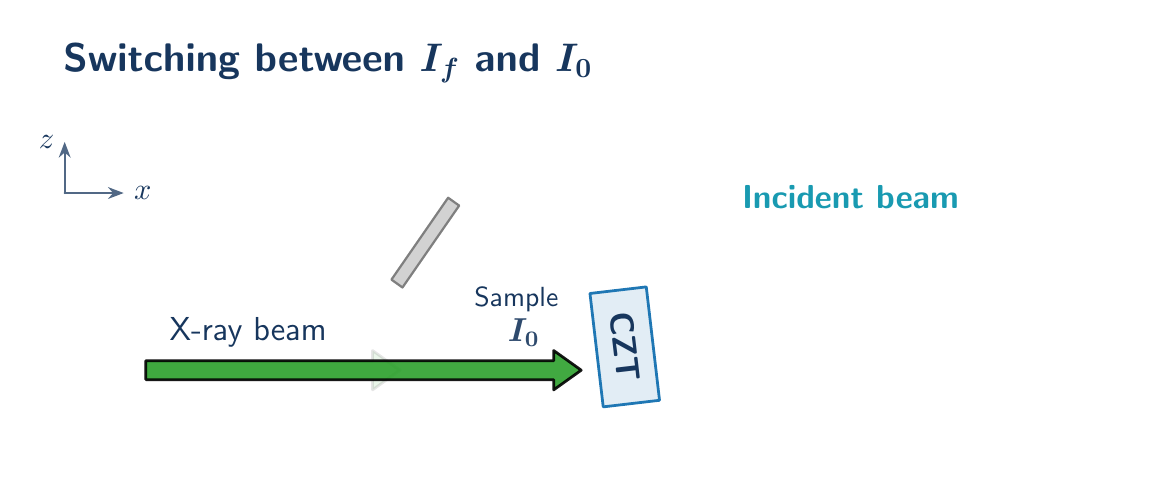
\begin{tikzpicture}[x=1cm,y=1cm,line join=round,line cap=round,
 every node/.style={font=\sffamily\fontsize{12}{14}\selectfont,text=ink},
]
\newcommand{\BeamArrow}[4]{%
  \begin{scope}
    \coordinate (beamStart) at #3;
    \coordinate (beamEnd) at #4;
    \path let \p1 = ($(beamEnd)-(beamStart)$),
      \n1 = {atan2(\y1,\x1)}, \n2 = {veclen(\x1,\y1)} in
      \pgfextra{\xdef\beamAngle{\n1}\xdef\beamLength{\n2}};
    \begin{scope}[shift={(beamStart)},rotate=\beamAngle]
      \path[fill=#1,draw=black,opacity=#2,line width=.35mm,line join=round]
        (0,-1.2mm) -- (\beamLength-3.5mm,-1.2mm)
        -- (\beamLength-3.5mm,-2.5mm) -- (\beamLength,0)
        -- (\beamLength-3.5mm,2.5mm) -- (\beamLength-3.5mm,1.2mm)
        -- (0,1.2mm) -- cycle;
    \end{scope}
  \end{scope}
}
\path[use as bounding box] (-1.05,-1.25) rectangle (12.8878,4.35);
\node[anchor=west,font=\sffamily\bfseries\fontsize{14}{17}\selectfont] at (-.72,3.9) {Switching between $\bm{I_f}$ and $\bm{I_0}$};
\draw[ink!75,line width=.8pt,-{Stealth[length=2mm]}] (-.58,2.25) -- (.17,2.25) node[anchor=west,font=\sffamily\fontsize{11}{13}\selectfont] {$x$};
\draw[ink!75,line width=.8pt,-{Stealth[length=2mm]}] (-.58,2.25) -- (-.58,2.9) node[anchor=east,font=\sffamily\fontsize{11}{13}\selectfont] {$z$};
\BeamArrow{beamgreen}{0.0992}{(.45,0)}{(3.68,0)}
\node at (1.75,.48) {X-ray beam};
\BeamArrow{beamgreen}{0.9008}{(.45,0)}{(5.98,0)}
\BeamArrow{fluororange}{0.0000}{(4,.35)}{(4,2.03)}
\node[opacity=0.0000,anchor=west] at (4.35,1.25) {$\bm{I_f}$};
\node[opacity=0.9008] at (5.25,.48) {$\bm{I_0}$};
\begin{scope}[shift={(4,1.6204)}]
\path[draw=samplegray,fill=samplegray!35,line width=.8pt] (-.43,-.47) -- (-.29,-.57) -- (.43,.47) -- (.29,.57) -- cycle;
\end{scope}
\node[anchor=west,font=\sffamily\fontsize{10}{12}\selectfont] at (4.5,0.9004) {Sample};
\begin{scope}[shift={(6.5328,0.2960)},rotate=-83.3333,transform shape]
\node[draw=detectorblue,fill=detectorblue!13,line width=1pt,minimum width=1.45cm,minimum height=.72cm,inner sep=2pt,font=\sffamily\bfseries\fontsize{13}{15}\selectfont] {CZT};
\end{scope}
\node[opacity=0.0000,font=\sffamily\bfseries\fontsize{13}{15}\selectfont,text=motioncyan] at (9.4,2.2) {Fluorescence};
\node[opacity=0.9008,font=\sffamily\bfseries\fontsize{13}{15}\selectfont,text=motioncyan] at (9.4,2.2) {Incident beam};
\end{tikzpicture}
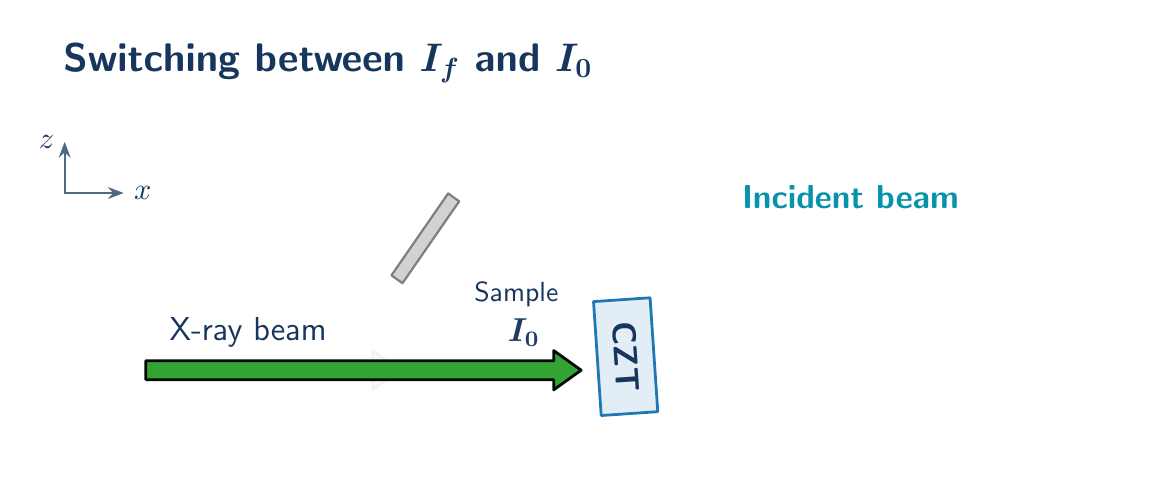
\begin{tikzpicture}[x=1cm,y=1cm,line join=round,line cap=round,
 every node/.style={font=\sffamily\fontsize{12}{14}\selectfont,text=ink},
]
\newcommand{\BeamArrow}[4]{%
  \begin{scope}
    \coordinate (beamStart) at #3;
    \coordinate (beamEnd) at #4;
    \path let \p1 = ($(beamEnd)-(beamStart)$),
      \n1 = {atan2(\y1,\x1)}, \n2 = {veclen(\x1,\y1)} in
      \pgfextra{\xdef\beamAngle{\n1}\xdef\beamLength{\n2}};
    \begin{scope}[shift={(beamStart)},rotate=\beamAngle]
      \path[fill=#1,draw=black,opacity=#2,line width=.35mm,line join=round]
        (0,-1.2mm) -- (\beamLength-3.5mm,-1.2mm)
        -- (\beamLength-3.5mm,-2.5mm) -- (\beamLength,0)
        -- (\beamLength-3.5mm,2.5mm) -- (\beamLength-3.5mm,1.2mm)
        -- (0,1.2mm) -- cycle;
    \end{scope}
  \end{scope}
}
\path[use as bounding box] (-1.05,-1.25) rectangle (12.8878,4.35);
\node[anchor=west,font=\sffamily\bfseries\fontsize{14}{17}\selectfont] at (-.72,3.9) {Switching between $\bm{I_f}$ and $\bm{I_0}$};
\draw[ink!75,line width=.8pt,-{Stealth[length=2mm]}] (-.58,2.25) -- (.17,2.25) node[anchor=west,font=\sffamily\fontsize{11}{13}\selectfont] {$x$};
\draw[ink!75,line width=.8pt,-{Stealth[length=2mm]}] (-.58,2.25) -- (-.58,2.9) node[anchor=east,font=\sffamily\fontsize{11}{13}\selectfont] {$z$};
\BeamArrow{beamgreen}{0.0355}{(.45,0)}{(3.68,0)}
\node at (1.75,.48) {X-ray beam};
\BeamArrow{beamgreen}{0.9645}{(.45,0)}{(5.98,0)}
\BeamArrow{fluororange}{0.0000}{(4,.35)}{(4,2.03)}
\node[opacity=0.0000,anchor=west] at (4.35,1.25) {$\bm{I_f}$};
\node[opacity=0.9645] at (5.25,.48) {$\bm{I_0}$};
\begin{scope}[shift={(4,1.6748)}]
\path[draw=samplegray,fill=samplegray!35,line width=.8pt] (-.43,-.47) -- (-.29,-.57) -- (.43,.47) -- (.29,.57) -- cycle;
\end{scope}
\node[anchor=west,font=\sffamily\fontsize{10}{12}\selectfont] at (4.5,0.9548) {Sample};
\begin{scope}[shift={(6.5442,0.1720)},rotate=-86.1328,transform shape]
\node[draw=detectorblue,fill=detectorblue!13,line width=1pt,minimum width=1.45cm,minimum height=.72cm,inner sep=2pt,font=\sffamily\bfseries\fontsize{13}{15}\selectfont] {CZT};
\end{scope}
\node[opacity=0.0000,font=\sffamily\bfseries\fontsize{13}{15}\selectfont,text=motioncyan] at (9.4,2.2) {Fluorescence};
\node[opacity=0.9645,font=\sffamily\bfseries\fontsize{13}{15}\selectfont,text=motioncyan] at (9.4,2.2) {Incident beam};
\end{tikzpicture}
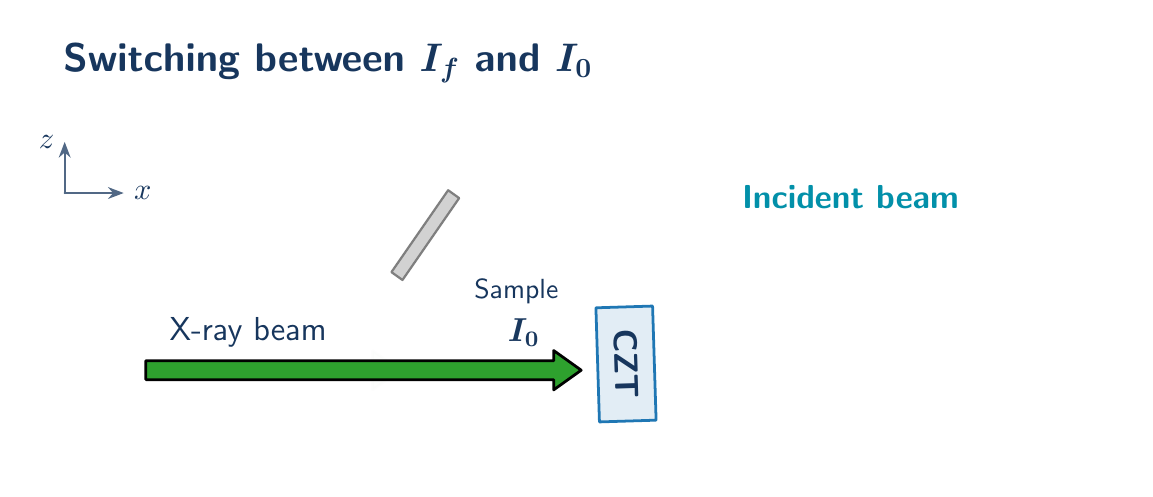
\begin{tikzpicture}[x=1cm,y=1cm,line join=round,line cap=round,
 every node/.style={font=\sffamily\fontsize{12}{14}\selectfont,text=ink},
]
\newcommand{\BeamArrow}[4]{%
  \begin{scope}
    \coordinate (beamStart) at #3;
    \coordinate (beamEnd) at #4;
    \path let \p1 = ($(beamEnd)-(beamStart)$),
      \n1 = {atan2(\y1,\x1)}, \n2 = {veclen(\x1,\y1)} in
      \pgfextra{\xdef\beamAngle{\n1}\xdef\beamLength{\n2}};
    \begin{scope}[shift={(beamStart)},rotate=\beamAngle]
      \path[fill=#1,draw=black,opacity=#2,line width=.35mm,line join=round]
        (0,-1.2mm) -- (\beamLength-3.5mm,-1.2mm)
        -- (\beamLength-3.5mm,-2.5mm) -- (\beamLength,0)
        -- (\beamLength-3.5mm,2.5mm) -- (\beamLength-3.5mm,1.2mm)
        -- (0,1.2mm) -- cycle;
    \end{scope}
  \end{scope}
}
\path[use as bounding box] (-1.05,-1.25) rectangle (12.8878,4.35);
\node[anchor=west,font=\sffamily\bfseries\fontsize{14}{17}\selectfont] at (-.72,3.9) {Switching between $\bm{I_f}$ and $\bm{I_0}$};
\draw[ink!75,line width=.8pt,-{Stealth[length=2mm]}] (-.58,2.25) -- (.17,2.25) node[anchor=west,font=\sffamily\fontsize{11}{13}\selectfont] {$x$};
\draw[ink!75,line width=.8pt,-{Stealth[length=2mm]}] (-.58,2.25) -- (-.58,2.9) node[anchor=east,font=\sffamily\fontsize{11}{13}\selectfont] {$z$};
\BeamArrow{beamgreen}{0.0078}{(.45,0)}{(3.68,0)}
\node at (1.75,.48) {X-ray beam};
\BeamArrow{beamgreen}{0.9922}{(.45,0)}{(5.98,0)}
\BeamArrow{fluororange}{0.0000}{(4,.35)}{(4,2.03)}
\node[opacity=0.0000,anchor=west] at (4.35,1.25) {$\bm{I_f}$};
\node[opacity=0.9922] at (5.25,.48) {$\bm{I_0}$};
\begin{scope}[shift={(4,1.7156)}]
\path[draw=samplegray,fill=samplegray!35,line width=.8pt] (-.43,-.47) -- (-.29,-.57) -- (.43,.47) -- (.29,.57) -- cycle;
\end{scope}
\node[anchor=west,font=\sffamily\fontsize{10}{12}\selectfont] at (4.5,0.9956) {Sample};
\begin{scope}[shift={(6.5488,0.0788)},rotate=-88.2292,transform shape]
\node[draw=detectorblue,fill=detectorblue!13,line width=1pt,minimum width=1.45cm,minimum height=.72cm,inner sep=2pt,font=\sffamily\bfseries\fontsize{13}{15}\selectfont] {CZT};
\end{scope}
\node[opacity=0.0000,font=\sffamily\bfseries\fontsize{13}{15}\selectfont,text=motioncyan] at (9.4,2.2) {Fluorescence};
\node[opacity=0.9922,font=\sffamily\bfseries\fontsize{13}{15}\selectfont,text=motioncyan] at (9.4,2.2) {Incident beam};
\end{tikzpicture}
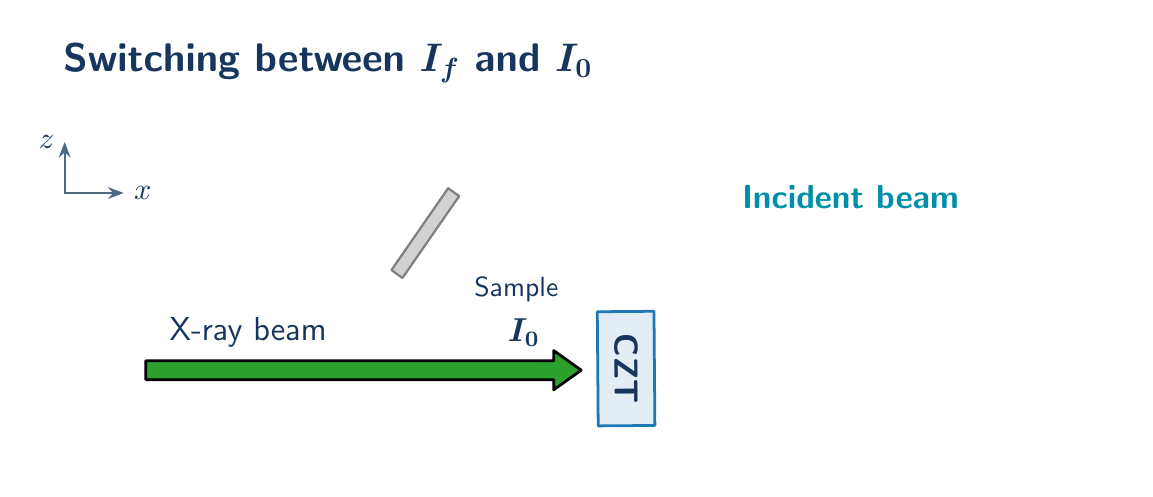
\begin{tikzpicture}[x=1cm,y=1cm,line join=round,line cap=round,
 every node/.style={font=\sffamily\fontsize{12}{14}\selectfont,text=ink},
]
\newcommand{\BeamArrow}[4]{%
  \begin{scope}
    \coordinate (beamStart) at #3;
    \coordinate (beamEnd) at #4;
    \path let \p1 = ($(beamEnd)-(beamStart)$),
      \n1 = {atan2(\y1,\x1)}, \n2 = {veclen(\x1,\y1)} in
      \pgfextra{\xdef\beamAngle{\n1}\xdef\beamLength{\n2}};
    \begin{scope}[shift={(beamStart)},rotate=\beamAngle]
      \path[fill=#1,draw=black,opacity=#2,line width=.35mm,line join=round]
        (0,-1.2mm) -- (\beamLength-3.5mm,-1.2mm)
        -- (\beamLength-3.5mm,-2.5mm) -- (\beamLength,0)
        -- (\beamLength-3.5mm,2.5mm) -- (\beamLength-3.5mm,1.2mm)
        -- (0,1.2mm) -- cycle;
    \end{scope}
  \end{scope}
}
\path[use as bounding box] (-1.05,-1.25) rectangle (12.8878,4.35);
\node[anchor=west,font=\sffamily\bfseries\fontsize{14}{17}\selectfont] at (-.72,3.9) {Switching between $\bm{I_f}$ and $\bm{I_0}$};
\draw[ink!75,line width=.8pt,-{Stealth[length=2mm]}] (-.58,2.25) -- (.17,2.25) node[anchor=west,font=\sffamily\fontsize{11}{13}\selectfont] {$x$};
\draw[ink!75,line width=.8pt,-{Stealth[length=2mm]}] (-.58,2.25) -- (-.58,2.9) node[anchor=east,font=\sffamily\fontsize{11}{13}\selectfont] {$z$};
\BeamArrow{beamgreen}{0.0005}{(.45,0)}{(3.68,0)}
\node at (1.75,.48) {X-ray beam};
\BeamArrow{beamgreen}{0.9995}{(.45,0)}{(5.98,0)}
\BeamArrow{fluororange}{0.0000}{(4,.35)}{(4,2.03)}
\node[opacity=0.0000,anchor=west] at (4.35,1.25) {$\bm{I_f}$};
\node[opacity=0.9995] at (5.25,.48) {$\bm{I_0}$};
\begin{scope}[shift={(4,1.7411)}]
\path[draw=samplegray,fill=samplegray!35,line width=.8pt] (-.43,-.47) -- (-.29,-.57) -- (.43,.47) -- (.29,.57) -- cycle;
\end{scope}
\node[anchor=west,font=\sffamily\fontsize{10}{12}\selectfont] at (4.5,1.0211) {Sample};
\begin{scope}[shift={(6.5499,0.0203)},rotate=-89.5443,transform shape]
\node[draw=detectorblue,fill=detectorblue!13,line width=1pt,minimum width=1.45cm,minimum height=.72cm,inner sep=2pt,font=\sffamily\bfseries\fontsize{13}{15}\selectfont] {CZT};
\end{scope}
\node[opacity=0.0000,font=\sffamily\bfseries\fontsize{13}{15}\selectfont,text=motioncyan] at (9.4,2.2) {Fluorescence};
\node[opacity=0.9995,font=\sffamily\bfseries\fontsize{13}{15}\selectfont,text=motioncyan] at (9.4,2.2) {Incident beam};
\end{tikzpicture}
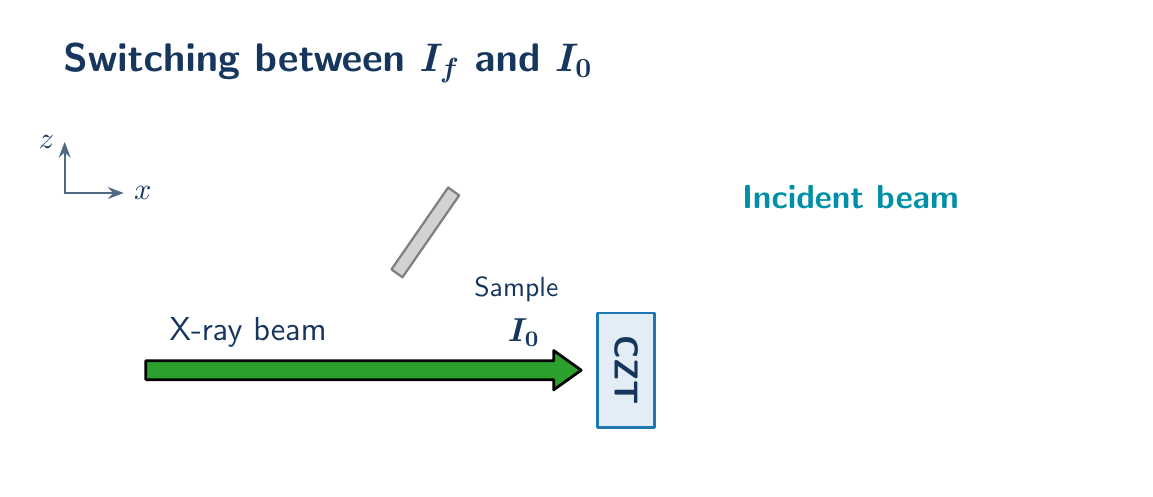
\begin{tikzpicture}[x=1cm,y=1cm,line join=round,line cap=round,
 every node/.style={font=\sffamily\fontsize{12}{14}\selectfont,text=ink},
]
\newcommand{\BeamArrow}[4]{%
  \begin{scope}
    \coordinate (beamStart) at #3;
    \coordinate (beamEnd) at #4;
    \path let \p1 = ($(beamEnd)-(beamStart)$),
      \n1 = {atan2(\y1,\x1)}, \n2 = {veclen(\x1,\y1)} in
      \pgfextra{\xdef\beamAngle{\n1}\xdef\beamLength{\n2}};
    \begin{scope}[shift={(beamStart)},rotate=\beamAngle]
      \path[fill=#1,draw=black,opacity=#2,line width=.35mm,line join=round]
        (0,-1.2mm) -- (\beamLength-3.5mm,-1.2mm)
        -- (\beamLength-3.5mm,-2.5mm) -- (\beamLength,0)
        -- (\beamLength-3.5mm,2.5mm) -- (\beamLength-3.5mm,1.2mm)
        -- (0,1.2mm) -- cycle;
    \end{scope}
  \end{scope}
}
\path[use as bounding box] (-1.05,-1.25) rectangle (12.8878,4.35);
\node[anchor=west,font=\sffamily\bfseries\fontsize{14}{17}\selectfont] at (-.72,3.9) {Switching between $\bm{I_f}$ and $\bm{I_0}$};
\draw[ink!75,line width=.8pt,-{Stealth[length=2mm]}] (-.58,2.25) -- (.17,2.25) node[anchor=west,font=\sffamily\fontsize{11}{13}\selectfont] {$x$};
\draw[ink!75,line width=.8pt,-{Stealth[length=2mm]}] (-.58,2.25) -- (-.58,2.9) node[anchor=east,font=\sffamily\fontsize{11}{13}\selectfont] {$z$};
\BeamArrow{beamgreen}{0.0000}{(.45,0)}{(3.68,0)}
\node at (1.75,.48) {X-ray beam};
\BeamArrow{beamgreen}{1.0000}{(.45,0)}{(5.98,0)}
\BeamArrow{fluororange}{0.0000}{(4,.35)}{(4,2.03)}
\node[opacity=0.0000,anchor=west] at (4.35,1.25) {$\bm{I_f}$};
\node[opacity=1.0000] at (5.25,.48) {$\bm{I_0}$};
\begin{scope}[shift={(4,1.7500)}]
\path[draw=samplegray,fill=samplegray!35,line width=.8pt] (-.43,-.47) -- (-.29,-.57) -- (.43,.47) -- (.29,.57) -- cycle;
\end{scope}
\node[anchor=west,font=\sffamily\fontsize{10}{12}\selectfont] at (4.5,1.0300) {Sample};
\begin{scope}[shift={(6.5500,0.0000)},rotate=-90.0000,transform shape]
\node[draw=detectorblue,fill=detectorblue!13,line width=1pt,minimum width=1.45cm,minimum height=.72cm,inner sep=2pt,font=\sffamily\bfseries\fontsize{13}{15}\selectfont] {CZT};
\end{scope}
\node[opacity=0.0000,font=\sffamily\bfseries\fontsize{13}{15}\selectfont,text=motioncyan] at (9.4,2.2) {Fluorescence};
\node[opacity=1.0000,font=\sffamily\bfseries\fontsize{13}{15}\selectfont,text=motioncyan] at (9.4,2.2) {Incident beam};
\end{tikzpicture}
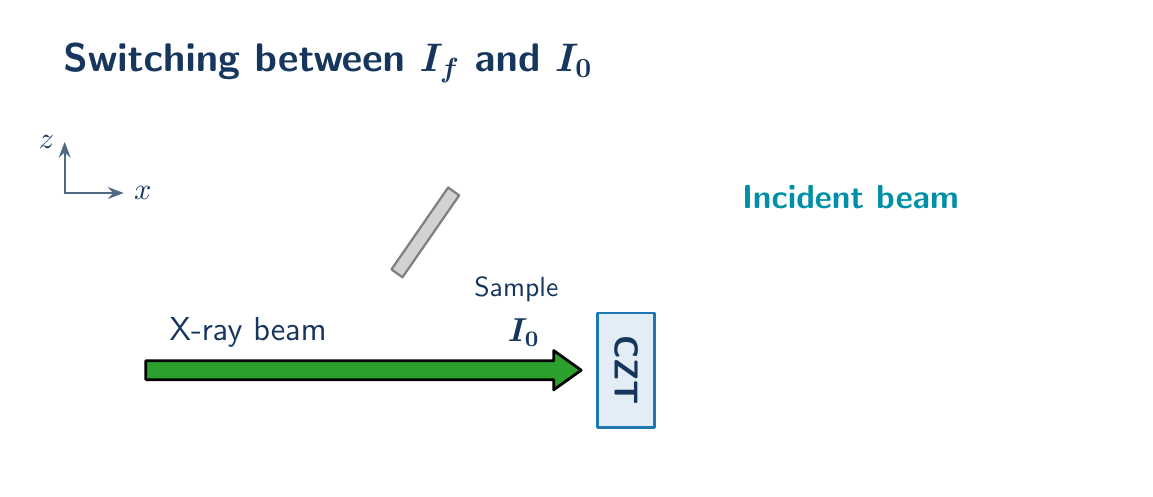
\begin{tikzpicture}[x=1cm,y=1cm,line join=round,line cap=round,
 every node/.style={font=\sffamily\fontsize{12}{14}\selectfont,text=ink},
]
\newcommand{\BeamArrow}[4]{%
  \begin{scope}
    \coordinate (beamStart) at #3;
    \coordinate (beamEnd) at #4;
    \path let \p1 = ($(beamEnd)-(beamStart)$),
      \n1 = {atan2(\y1,\x1)}, \n2 = {veclen(\x1,\y1)} in
      \pgfextra{\xdef\beamAngle{\n1}\xdef\beamLength{\n2}};
    \begin{scope}[shift={(beamStart)},rotate=\beamAngle]
      \path[fill=#1,draw=black,opacity=#2,line width=.35mm,line join=round]
        (0,-1.2mm) -- (\beamLength-3.5mm,-1.2mm)
        -- (\beamLength-3.5mm,-2.5mm) -- (\beamLength,0)
        -- (\beamLength-3.5mm,2.5mm) -- (\beamLength-3.5mm,1.2mm)
        -- (0,1.2mm) -- cycle;
    \end{scope}
  \end{scope}
}
\path[use as bounding box] (-1.05,-1.25) rectangle (12.8878,4.35);
\node[anchor=west,font=\sffamily\bfseries\fontsize{14}{17}\selectfont] at (-.72,3.9) {Switching between $\bm{I_f}$ and $\bm{I_0}$};
\draw[ink!75,line width=.8pt,-{Stealth[length=2mm]}] (-.58,2.25) -- (.17,2.25) node[anchor=west,font=\sffamily\fontsize{11}{13}\selectfont] {$x$};
\draw[ink!75,line width=.8pt,-{Stealth[length=2mm]}] (-.58,2.25) -- (-.58,2.9) node[anchor=east,font=\sffamily\fontsize{11}{13}\selectfont] {$z$};
\BeamArrow{beamgreen}{0.0000}{(.45,0)}{(3.68,0)}
\node at (1.75,.48) {X-ray beam};
\BeamArrow{beamgreen}{1.0000}{(.45,0)}{(5.98,0)}
\BeamArrow{fluororange}{0.0000}{(4,.35)}{(4,2.03)}
\node[opacity=0.0000,anchor=west] at (4.35,1.25) {$\bm{I_f}$};
\node[opacity=1.0000] at (5.25,.48) {$\bm{I_0}$};
\begin{scope}[shift={(4,1.7500)}]
\path[draw=samplegray,fill=samplegray!35,line width=.8pt] (-.43,-.47) -- (-.29,-.57) -- (.43,.47) -- (.29,.57) -- cycle;
\end{scope}
\node[anchor=west,font=\sffamily\fontsize{10}{12}\selectfont] at (4.5,1.0300) {Sample};
\begin{scope}[shift={(6.5500,0.0000)},rotate=-90.0000,transform shape]
\node[draw=detectorblue,fill=detectorblue!13,line width=1pt,minimum width=1.45cm,minimum height=.72cm,inner sep=2pt,font=\sffamily\bfseries\fontsize{13}{15}\selectfont] {CZT};
\end{scope}
\node[opacity=0.0000,font=\sffamily\bfseries\fontsize{13}{15}\selectfont,text=motioncyan] at (9.4,2.2) {Fluorescence};
\node[opacity=1.0000,font=\sffamily\bfseries\fontsize{13}{15}\selectfont,text=motioncyan] at (9.4,2.2) {Incident beam};
\end{tikzpicture}
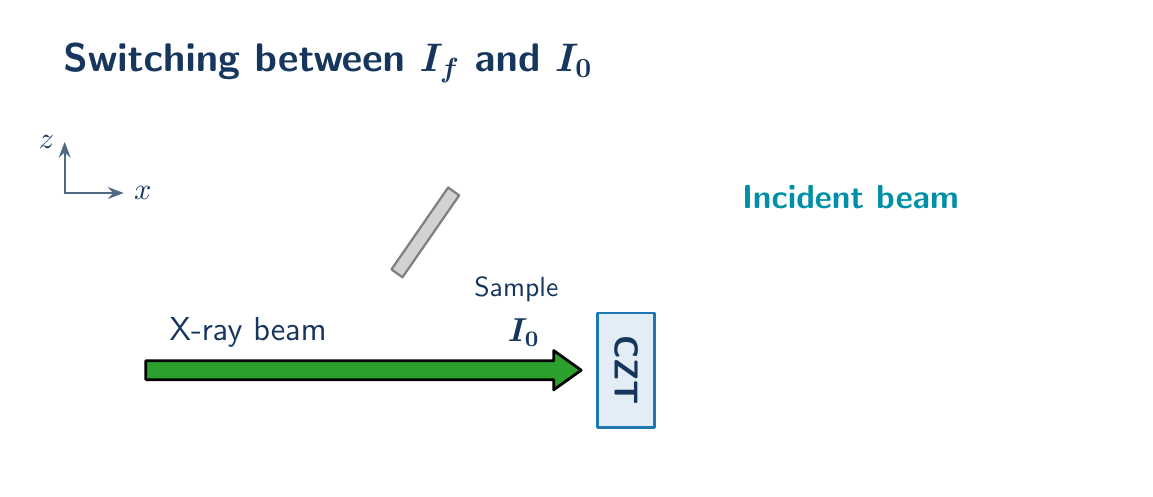
\begin{tikzpicture}[x=1cm,y=1cm,line join=round,line cap=round,
 every node/.style={font=\sffamily\fontsize{12}{14}\selectfont,text=ink},
]
\newcommand{\BeamArrow}[4]{%
  \begin{scope}
    \coordinate (beamStart) at #3;
    \coordinate (beamEnd) at #4;
    \path let \p1 = ($(beamEnd)-(beamStart)$),
      \n1 = {atan2(\y1,\x1)}, \n2 = {veclen(\x1,\y1)} in
      \pgfextra{\xdef\beamAngle{\n1}\xdef\beamLength{\n2}};
    \begin{scope}[shift={(beamStart)},rotate=\beamAngle]
      \path[fill=#1,draw=black,opacity=#2,line width=.35mm,line join=round]
        (0,-1.2mm) -- (\beamLength-3.5mm,-1.2mm)
        -- (\beamLength-3.5mm,-2.5mm) -- (\beamLength,0)
        -- (\beamLength-3.5mm,2.5mm) -- (\beamLength-3.5mm,1.2mm)
        -- (0,1.2mm) -- cycle;
    \end{scope}
  \end{scope}
}
\path[use as bounding box] (-1.05,-1.25) rectangle (12.8878,4.35);
\node[anchor=west,font=\sffamily\bfseries\fontsize{14}{17}\selectfont] at (-.72,3.9) {Switching between $\bm{I_f}$ and $\bm{I_0}$};
\draw[ink!75,line width=.8pt,-{Stealth[length=2mm]}] (-.58,2.25) -- (.17,2.25) node[anchor=west,font=\sffamily\fontsize{11}{13}\selectfont] {$x$};
\draw[ink!75,line width=.8pt,-{Stealth[length=2mm]}] (-.58,2.25) -- (-.58,2.9) node[anchor=east,font=\sffamily\fontsize{11}{13}\selectfont] {$z$};
\BeamArrow{beamgreen}{0.0000}{(.45,0)}{(3.68,0)}
\node at (1.75,.48) {X-ray beam};
\BeamArrow{beamgreen}{1.0000}{(.45,0)}{(5.98,0)}
\BeamArrow{fluororange}{0.0000}{(4,.35)}{(4,2.03)}
\node[opacity=0.0000,anchor=west] at (4.35,1.25) {$\bm{I_f}$};
\node[opacity=1.0000] at (5.25,.48) {$\bm{I_0}$};
\begin{scope}[shift={(4,1.7500)}]
\path[draw=samplegray,fill=samplegray!35,line width=.8pt] (-.43,-.47) -- (-.29,-.57) -- (.43,.47) -- (.29,.57) -- cycle;
\end{scope}
\node[anchor=west,font=\sffamily\fontsize{10}{12}\selectfont] at (4.5,1.0300) {Sample};
\begin{scope}[shift={(6.5500,0.0000)},rotate=-90.0000,transform shape]
\node[draw=detectorblue,fill=detectorblue!13,line width=1pt,minimum width=1.45cm,minimum height=.72cm,inner sep=2pt,font=\sffamily\bfseries\fontsize{13}{15}\selectfont] {CZT};
\end{scope}
\node[opacity=0.0000,font=\sffamily\bfseries\fontsize{13}{15}\selectfont,text=motioncyan] at (9.4,2.2) {Fluorescence};
\node[opacity=1.0000,font=\sffamily\bfseries\fontsize{13}{15}\selectfont,text=motioncyan] at (9.4,2.2) {Incident beam};
\end{tikzpicture}
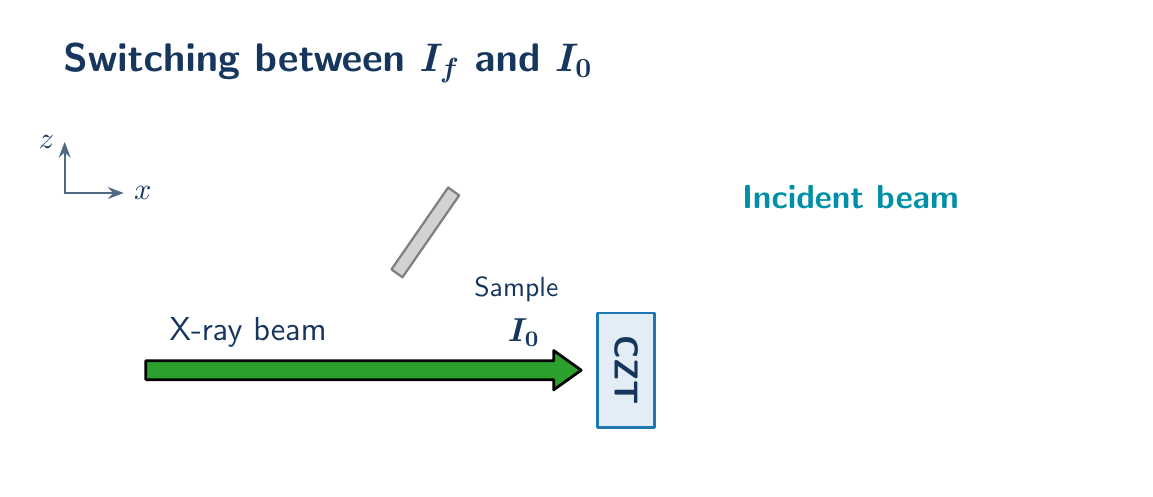
\begin{tikzpicture}[x=1cm,y=1cm,line join=round,line cap=round,
 every node/.style={font=\sffamily\fontsize{12}{14}\selectfont,text=ink},
]
\newcommand{\BeamArrow}[4]{%
  \begin{scope}
    \coordinate (beamStart) at #3;
    \coordinate (beamEnd) at #4;
    \path let \p1 = ($(beamEnd)-(beamStart)$),
      \n1 = {atan2(\y1,\x1)}, \n2 = {veclen(\x1,\y1)} in
      \pgfextra{\xdef\beamAngle{\n1}\xdef\beamLength{\n2}};
    \begin{scope}[shift={(beamStart)},rotate=\beamAngle]
      \path[fill=#1,draw=black,opacity=#2,line width=.35mm,line join=round]
        (0,-1.2mm) -- (\beamLength-3.5mm,-1.2mm)
        -- (\beamLength-3.5mm,-2.5mm) -- (\beamLength,0)
        -- (\beamLength-3.5mm,2.5mm) -- (\beamLength-3.5mm,1.2mm)
        -- (0,1.2mm) -- cycle;
    \end{scope}
  \end{scope}
}
\path[use as bounding box] (-1.05,-1.25) rectangle (12.8878,4.35);
\node[anchor=west,font=\sffamily\bfseries\fontsize{14}{17}\selectfont] at (-.72,3.9) {Switching between $\bm{I_f}$ and $\bm{I_0}$};
\draw[ink!75,line width=.8pt,-{Stealth[length=2mm]}] (-.58,2.25) -- (.17,2.25) node[anchor=west,font=\sffamily\fontsize{11}{13}\selectfont] {$x$};
\draw[ink!75,line width=.8pt,-{Stealth[length=2mm]}] (-.58,2.25) -- (-.58,2.9) node[anchor=east,font=\sffamily\fontsize{11}{13}\selectfont] {$z$};
\BeamArrow{beamgreen}{0.0000}{(.45,0)}{(3.68,0)}
\node at (1.75,.48) {X-ray beam};
\BeamArrow{beamgreen}{1.0000}{(.45,0)}{(5.98,0)}
\BeamArrow{fluororange}{0.0000}{(4,.35)}{(4,2.03)}
\node[opacity=0.0000,anchor=west] at (4.35,1.25) {$\bm{I_f}$};
\node[opacity=1.0000] at (5.25,.48) {$\bm{I_0}$};
\begin{scope}[shift={(4,1.7500)}]
\path[draw=samplegray,fill=samplegray!35,line width=.8pt] (-.43,-.47) -- (-.29,-.57) -- (.43,.47) -- (.29,.57) -- cycle;
\end{scope}
\node[anchor=west,font=\sffamily\fontsize{10}{12}\selectfont] at (4.5,1.0300) {Sample};
\begin{scope}[shift={(6.5500,0.0000)},rotate=-90.0000,transform shape]
\node[draw=detectorblue,fill=detectorblue!13,line width=1pt,minimum width=1.45cm,minimum height=.72cm,inner sep=2pt,font=\sffamily\bfseries\fontsize{13}{15}\selectfont] {CZT};
\end{scope}
\node[opacity=0.0000,font=\sffamily\bfseries\fontsize{13}{15}\selectfont,text=motioncyan] at (9.4,2.2) {Fluorescence};
\node[opacity=1.0000,font=\sffamily\bfseries\fontsize{13}{15}\selectfont,text=motioncyan] at (9.4,2.2) {Incident beam};
\end{tikzpicture}
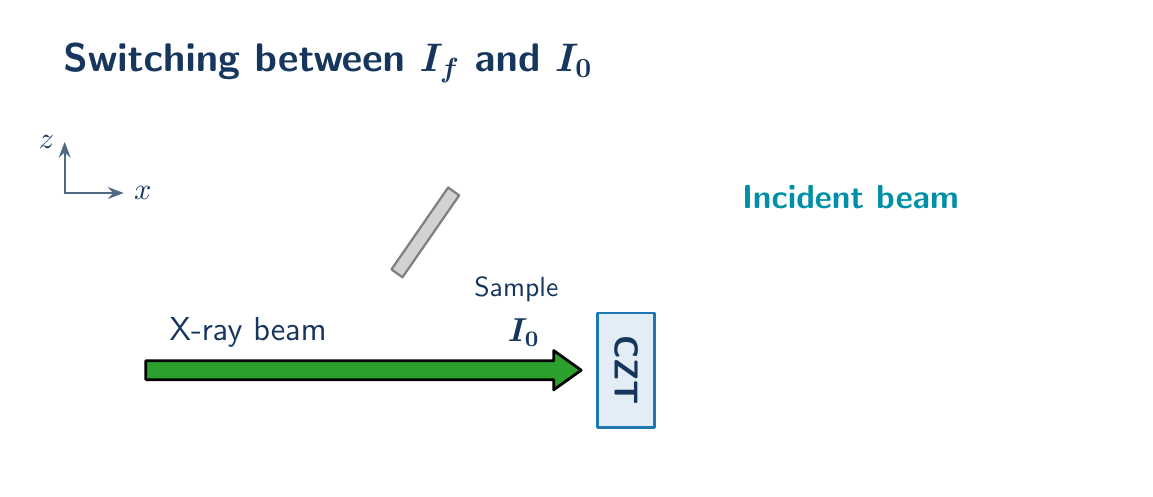
\begin{tikzpicture}[x=1cm,y=1cm,line join=round,line cap=round,
 every node/.style={font=\sffamily\fontsize{12}{14}\selectfont,text=ink},
]
\newcommand{\BeamArrow}[4]{%
  \begin{scope}
    \coordinate (beamStart) at #3;
    \coordinate (beamEnd) at #4;
    \path let \p1 = ($(beamEnd)-(beamStart)$),
      \n1 = {atan2(\y1,\x1)}, \n2 = {veclen(\x1,\y1)} in
      \pgfextra{\xdef\beamAngle{\n1}\xdef\beamLength{\n2}};
    \begin{scope}[shift={(beamStart)},rotate=\beamAngle]
      \path[fill=#1,draw=black,opacity=#2,line width=.35mm,line join=round]
        (0,-1.2mm) -- (\beamLength-3.5mm,-1.2mm)
        -- (\beamLength-3.5mm,-2.5mm) -- (\beamLength,0)
        -- (\beamLength-3.5mm,2.5mm) -- (\beamLength-3.5mm,1.2mm)
        -- (0,1.2mm) -- cycle;
    \end{scope}
  \end{scope}
}
\path[use as bounding box] (-1.05,-1.25) rectangle (12.8878,4.35);
\node[anchor=west,font=\sffamily\bfseries\fontsize{14}{17}\selectfont] at (-.72,3.9) {Switching between $\bm{I_f}$ and $\bm{I_0}$};
\draw[ink!75,line width=.8pt,-{Stealth[length=2mm]}] (-.58,2.25) -- (.17,2.25) node[anchor=west,font=\sffamily\fontsize{11}{13}\selectfont] {$x$};
\draw[ink!75,line width=.8pt,-{Stealth[length=2mm]}] (-.58,2.25) -- (-.58,2.9) node[anchor=east,font=\sffamily\fontsize{11}{13}\selectfont] {$z$};
\BeamArrow{beamgreen}{0.0000}{(.45,0)}{(3.68,0)}
\node at (1.75,.48) {X-ray beam};
\BeamArrow{beamgreen}{1.0000}{(.45,0)}{(5.98,0)}
\BeamArrow{fluororange}{0.0000}{(4,.35)}{(4,2.03)}
\node[opacity=0.0000,anchor=west] at (4.35,1.25) {$\bm{I_f}$};
\node[opacity=1.0000] at (5.25,.48) {$\bm{I_0}$};
\begin{scope}[shift={(4,1.7500)}]
\path[draw=samplegray,fill=samplegray!35,line width=.8pt] (-.43,-.47) -- (-.29,-.57) -- (.43,.47) -- (.29,.57) -- cycle;
\end{scope}
\node[anchor=west,font=\sffamily\fontsize{10}{12}\selectfont] at (4.5,1.0300) {Sample};
\begin{scope}[shift={(6.5500,0.0000)},rotate=-90.0000,transform shape]
\node[draw=detectorblue,fill=detectorblue!13,line width=1pt,minimum width=1.45cm,minimum height=.72cm,inner sep=2pt,font=\sffamily\bfseries\fontsize{13}{15}\selectfont] {CZT};
\end{scope}
\node[opacity=0.0000,font=\sffamily\bfseries\fontsize{13}{15}\selectfont,text=motioncyan] at (9.4,2.2) {Fluorescence};
\node[opacity=1.0000,font=\sffamily\bfseries\fontsize{13}{15}\selectfont,text=motioncyan] at (9.4,2.2) {Incident beam};
\end{tikzpicture}
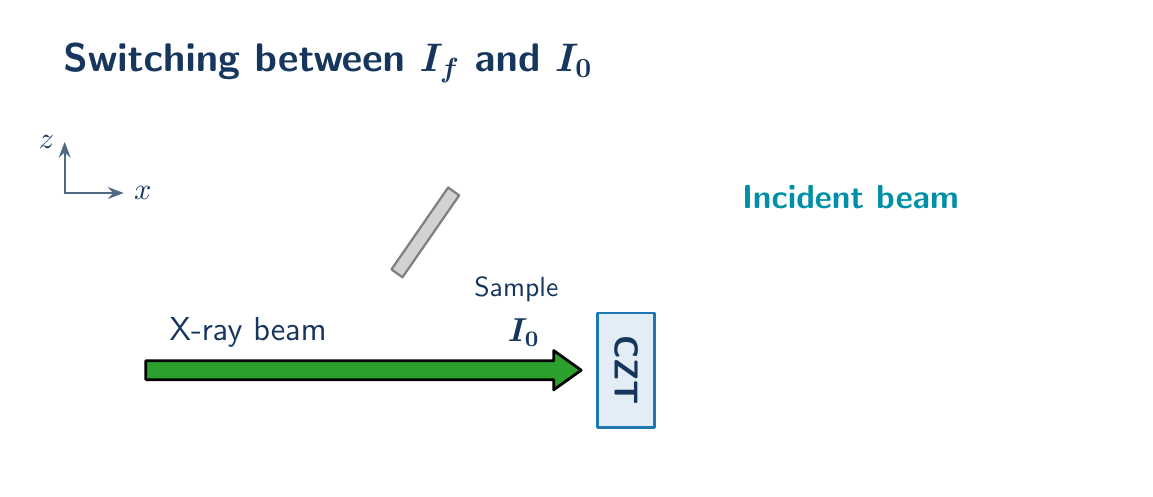
\begin{tikzpicture}[x=1cm,y=1cm,line join=round,line cap=round,
 every node/.style={font=\sffamily\fontsize{12}{14}\selectfont,text=ink},
]
\newcommand{\BeamArrow}[4]{%
  \begin{scope}
    \coordinate (beamStart) at #3;
    \coordinate (beamEnd) at #4;
    \path let \p1 = ($(beamEnd)-(beamStart)$),
      \n1 = {atan2(\y1,\x1)}, \n2 = {veclen(\x1,\y1)} in
      \pgfextra{\xdef\beamAngle{\n1}\xdef\beamLength{\n2}};
    \begin{scope}[shift={(beamStart)},rotate=\beamAngle]
      \path[fill=#1,draw=black,opacity=#2,line width=.35mm,line join=round]
        (0,-1.2mm) -- (\beamLength-3.5mm,-1.2mm)
        -- (\beamLength-3.5mm,-2.5mm) -- (\beamLength,0)
        -- (\beamLength-3.5mm,2.5mm) -- (\beamLength-3.5mm,1.2mm)
        -- (0,1.2mm) -- cycle;
    \end{scope}
  \end{scope}
}
\path[use as bounding box] (-1.05,-1.25) rectangle (12.8878,4.35);
\node[anchor=west,font=\sffamily\bfseries\fontsize{14}{17}\selectfont] at (-.72,3.9) {Switching between $\bm{I_f}$ and $\bm{I_0}$};
\draw[ink!75,line width=.8pt,-{Stealth[length=2mm]}] (-.58,2.25) -- (.17,2.25) node[anchor=west,font=\sffamily\fontsize{11}{13}\selectfont] {$x$};
\draw[ink!75,line width=.8pt,-{Stealth[length=2mm]}] (-.58,2.25) -- (-.58,2.9) node[anchor=east,font=\sffamily\fontsize{11}{13}\selectfont] {$z$};
\BeamArrow{beamgreen}{0.0000}{(.45,0)}{(3.68,0)}
\node at (1.75,.48) {X-ray beam};
\BeamArrow{beamgreen}{1.0000}{(.45,0)}{(5.98,0)}
\BeamArrow{fluororange}{0.0000}{(4,.35)}{(4,2.03)}
\node[opacity=0.0000,anchor=west] at (4.35,1.25) {$\bm{I_f}$};
\node[opacity=1.0000] at (5.25,.48) {$\bm{I_0}$};
\begin{scope}[shift={(4,1.7500)}]
\path[draw=samplegray,fill=samplegray!35,line width=.8pt] (-.43,-.47) -- (-.29,-.57) -- (.43,.47) -- (.29,.57) -- cycle;
\end{scope}
\node[anchor=west,font=\sffamily\fontsize{10}{12}\selectfont] at (4.5,1.0300) {Sample};
\begin{scope}[shift={(6.5500,0.0000)},rotate=-90.0000,transform shape]
\node[draw=detectorblue,fill=detectorblue!13,line width=1pt,minimum width=1.45cm,minimum height=.72cm,inner sep=2pt,font=\sffamily\bfseries\fontsize{13}{15}\selectfont] {CZT};
\end{scope}
\node[opacity=0.0000,font=\sffamily\bfseries\fontsize{13}{15}\selectfont,text=motioncyan] at (9.4,2.2) {Fluorescence};
\node[opacity=1.0000,font=\sffamily\bfseries\fontsize{13}{15}\selectfont,text=motioncyan] at (9.4,2.2) {Incident beam};
\end{tikzpicture}
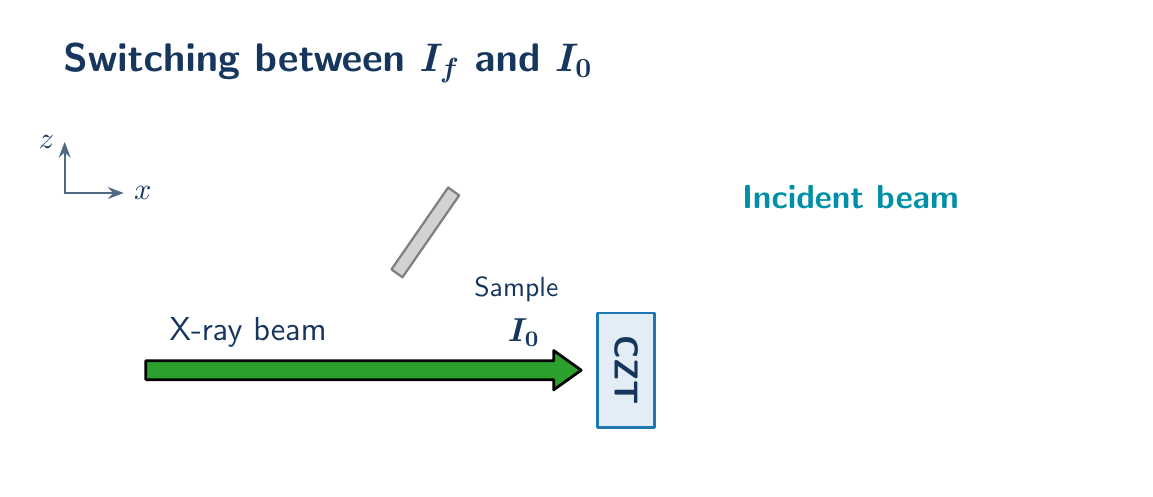
\begin{tikzpicture}[x=1cm,y=1cm,line join=round,line cap=round,
 every node/.style={font=\sffamily\fontsize{12}{14}\selectfont,text=ink},
]
\newcommand{\BeamArrow}[4]{%
  \begin{scope}
    \coordinate (beamStart) at #3;
    \coordinate (beamEnd) at #4;
    \path let \p1 = ($(beamEnd)-(beamStart)$),
      \n1 = {atan2(\y1,\x1)}, \n2 = {veclen(\x1,\y1)} in
      \pgfextra{\xdef\beamAngle{\n1}\xdef\beamLength{\n2}};
    \begin{scope}[shift={(beamStart)},rotate=\beamAngle]
      \path[fill=#1,draw=black,opacity=#2,line width=.35mm,line join=round]
        (0,-1.2mm) -- (\beamLength-3.5mm,-1.2mm)
        -- (\beamLength-3.5mm,-2.5mm) -- (\beamLength,0)
        -- (\beamLength-3.5mm,2.5mm) -- (\beamLength-3.5mm,1.2mm)
        -- (0,1.2mm) -- cycle;
    \end{scope}
  \end{scope}
}
\path[use as bounding box] (-1.05,-1.25) rectangle (12.8878,4.35);
\node[anchor=west,font=\sffamily\bfseries\fontsize{14}{17}\selectfont] at (-.72,3.9) {Switching between $\bm{I_f}$ and $\bm{I_0}$};
\draw[ink!75,line width=.8pt,-{Stealth[length=2mm]}] (-.58,2.25) -- (.17,2.25) node[anchor=west,font=\sffamily\fontsize{11}{13}\selectfont] {$x$};
\draw[ink!75,line width=.8pt,-{Stealth[length=2mm]}] (-.58,2.25) -- (-.58,2.9) node[anchor=east,font=\sffamily\fontsize{11}{13}\selectfont] {$z$};
\BeamArrow{beamgreen}{0.0000}{(.45,0)}{(3.68,0)}
\node at (1.75,.48) {X-ray beam};
\BeamArrow{beamgreen}{1.0000}{(.45,0)}{(5.98,0)}
\BeamArrow{fluororange}{0.0000}{(4,.35)}{(4,2.03)}
\node[opacity=0.0000,anchor=west] at (4.35,1.25) {$\bm{I_f}$};
\node[opacity=1.0000] at (5.25,.48) {$\bm{I_0}$};
\begin{scope}[shift={(4,1.7500)}]
\path[draw=samplegray,fill=samplegray!35,line width=.8pt] (-.43,-.47) -- (-.29,-.57) -- (.43,.47) -- (.29,.57) -- cycle;
\end{scope}
\node[anchor=west,font=\sffamily\fontsize{10}{12}\selectfont] at (4.5,1.0300) {Sample};
\begin{scope}[shift={(6.5500,0.0000)},rotate=-90.0000,transform shape]
\node[draw=detectorblue,fill=detectorblue!13,line width=1pt,minimum width=1.45cm,minimum height=.72cm,inner sep=2pt,font=\sffamily\bfseries\fontsize{13}{15}\selectfont] {CZT};
\end{scope}
\node[opacity=0.0000,font=\sffamily\bfseries\fontsize{13}{15}\selectfont,text=motioncyan] at (9.4,2.2) {Fluorescence};
\node[opacity=1.0000,font=\sffamily\bfseries\fontsize{13}{15}\selectfont,text=motioncyan] at (9.4,2.2) {Incident beam};
\end{tikzpicture}
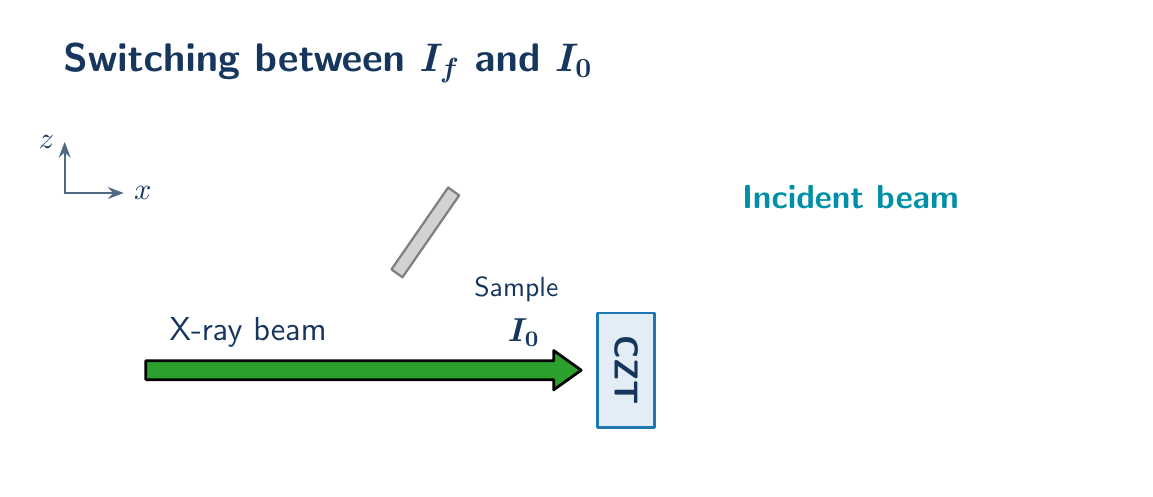
\begin{tikzpicture}[x=1cm,y=1cm,line join=round,line cap=round,
 every node/.style={font=\sffamily\fontsize{12}{14}\selectfont,text=ink},
]
\newcommand{\BeamArrow}[4]{%
  \begin{scope}
    \coordinate (beamStart) at #3;
    \coordinate (beamEnd) at #4;
    \path let \p1 = ($(beamEnd)-(beamStart)$),
      \n1 = {atan2(\y1,\x1)}, \n2 = {veclen(\x1,\y1)} in
      \pgfextra{\xdef\beamAngle{\n1}\xdef\beamLength{\n2}};
    \begin{scope}[shift={(beamStart)},rotate=\beamAngle]
      \path[fill=#1,draw=black,opacity=#2,line width=.35mm,line join=round]
        (0,-1.2mm) -- (\beamLength-3.5mm,-1.2mm)
        -- (\beamLength-3.5mm,-2.5mm) -- (\beamLength,0)
        -- (\beamLength-3.5mm,2.5mm) -- (\beamLength-3.5mm,1.2mm)
        -- (0,1.2mm) -- cycle;
    \end{scope}
  \end{scope}
}
\path[use as bounding box] (-1.05,-1.25) rectangle (12.8878,4.35);
\node[anchor=west,font=\sffamily\bfseries\fontsize{14}{17}\selectfont] at (-.72,3.9) {Switching between $\bm{I_f}$ and $\bm{I_0}$};
\draw[ink!75,line width=.8pt,-{Stealth[length=2mm]}] (-.58,2.25) -- (.17,2.25) node[anchor=west,font=\sffamily\fontsize{11}{13}\selectfont] {$x$};
\draw[ink!75,line width=.8pt,-{Stealth[length=2mm]}] (-.58,2.25) -- (-.58,2.9) node[anchor=east,font=\sffamily\fontsize{11}{13}\selectfont] {$z$};
\BeamArrow{beamgreen}{0.0000}{(.45,0)}{(3.68,0)}
\node at (1.75,.48) {X-ray beam};
\BeamArrow{beamgreen}{1.0000}{(.45,0)}{(5.98,0)}
\BeamArrow{fluororange}{0.0000}{(4,.35)}{(4,2.03)}
\node[opacity=0.0000,anchor=west] at (4.35,1.25) {$\bm{I_f}$};
\node[opacity=1.0000] at (5.25,.48) {$\bm{I_0}$};
\begin{scope}[shift={(4,1.7500)}]
\path[draw=samplegray,fill=samplegray!35,line width=.8pt] (-.43,-.47) -- (-.29,-.57) -- (.43,.47) -- (.29,.57) -- cycle;
\end{scope}
\node[anchor=west,font=\sffamily\fontsize{10}{12}\selectfont] at (4.5,1.0300) {Sample};
\begin{scope}[shift={(6.5500,0.0000)},rotate=-90.0000,transform shape]
\node[draw=detectorblue,fill=detectorblue!13,line width=1pt,minimum width=1.45cm,minimum height=.72cm,inner sep=2pt,font=\sffamily\bfseries\fontsize{13}{15}\selectfont] {CZT};
\end{scope}
\node[opacity=0.0000,font=\sffamily\bfseries\fontsize{13}{15}\selectfont,text=motioncyan] at (9.4,2.2) {Fluorescence};
\node[opacity=1.0000,font=\sffamily\bfseries\fontsize{13}{15}\selectfont,text=motioncyan] at (9.4,2.2) {Incident beam};
\end{tikzpicture}
\begin{tikzpicture}[x=1cm,y=1cm,line join=round,line cap=round,
 every node/.style={font=\sffamily\fontsize{12}{14}\selectfont,text=ink},
]
\newcommand{\BeamArrow}[4]{%
  \begin{scope}
    \coordinate (beamStart) at #3;
    \coordinate (beamEnd) at #4;
    \path let \p1 = ($(beamEnd)-(beamStart)$),
      \n1 = {atan2(\y1,\x1)}, \n2 = {veclen(\x1,\y1)} in
      \pgfextra{\xdef\beamAngle{\n1}\xdef\beamLength{\n2}};
    \begin{scope}[shift={(beamStart)},rotate=\beamAngle]
      \path[fill=#1,draw=black,opacity=#2,line width=.35mm,line join=round]
        (0,-1.2mm) -- (\beamLength-3.5mm,-1.2mm)
        -- (\beamLength-3.5mm,-2.5mm) -- (\beamLength,0)
        -- (\beamLength-3.5mm,2.5mm) -- (\beamLength-3.5mm,1.2mm)
        -- (0,1.2mm) -- cycle;
    \end{scope}
  \end{scope}
}
\path[use as bounding box] (-1.05,-1.25) rectangle (12.8878,4.35);
\node[anchor=west,font=\sffamily\bfseries\fontsize{14}{17}\selectfont] at (-.72,3.9) {Switching between $\bm{I_f}$ and $\bm{I_0}$};
\draw[ink!75,line width=.8pt,-{Stealth[length=2mm]}] (-.58,2.25) -- (.17,2.25) node[anchor=west,font=\sffamily\fontsize{11}{13}\selectfont] {$x$};
\draw[ink!75,line width=.8pt,-{Stealth[length=2mm]}] (-.58,2.25) -- (-.58,2.9) node[anchor=east,font=\sffamily\fontsize{11}{13}\selectfont] {$z$};
\BeamArrow{beamgreen}{0.0000}{(.45,0)}{(3.68,0)}
\node at (1.75,.48) {X-ray beam};
\BeamArrow{beamgreen}{1.0000}{(.45,0)}{(5.98,0)}
\BeamArrow{fluororange}{0.0000}{(4,.35)}{(4,2.03)}
\node[opacity=0.0000,anchor=west] at (4.35,1.25) {$\bm{I_f}$};
\node[opacity=1.0000] at (5.25,.48) {$\bm{I_0}$};
\begin{scope}[shift={(4,1.7500)}]
\path[draw=samplegray,fill=samplegray!35,line width=.8pt] (-.43,-.47) -- (-.29,-.57) -- (.43,.47) -- (.29,.57) -- cycle;
\end{scope}
\node[anchor=west,font=\sffamily\fontsize{10}{12}\selectfont] at (4.5,1.0300) {Sample};
\begin{scope}[shift={(6.5500,0.0000)},rotate=-90.0000,transform shape]
\node[draw=detectorblue,fill=detectorblue!13,line width=1pt,minimum width=1.45cm,minimum height=.72cm,inner sep=2pt,font=\sffamily\bfseries\fontsize{13}{15}\selectfont] {CZT};
\end{scope}
\node[opacity=0.0000,font=\sffamily\bfseries\fontsize{13}{15}\selectfont,text=motioncyan] at (9.4,2.2) {Fluorescence};
\node[opacity=1.0000,font=\sffamily\bfseries\fontsize{13}{15}\selectfont,text=motioncyan] at (9.4,2.2) {Incident beam};
\end{tikzpicture}
\begin{tikzpicture}[x=1cm,y=1cm,line join=round,line cap=round,
 every node/.style={font=\sffamily\fontsize{12}{14}\selectfont,text=ink},
]
\newcommand{\BeamArrow}[4]{%
  \begin{scope}
    \coordinate (beamStart) at #3;
    \coordinate (beamEnd) at #4;
    \path let \p1 = ($(beamEnd)-(beamStart)$),
      \n1 = {atan2(\y1,\x1)}, \n2 = {veclen(\x1,\y1)} in
      \pgfextra{\xdef\beamAngle{\n1}\xdef\beamLength{\n2}};
    \begin{scope}[shift={(beamStart)},rotate=\beamAngle]
      \path[fill=#1,draw=black,opacity=#2,line width=.35mm,line join=round]
        (0,-1.2mm) -- (\beamLength-3.5mm,-1.2mm)
        -- (\beamLength-3.5mm,-2.5mm) -- (\beamLength,0)
        -- (\beamLength-3.5mm,2.5mm) -- (\beamLength-3.5mm,1.2mm)
        -- (0,1.2mm) -- cycle;
    \end{scope}
  \end{scope}
}
\path[use as bounding box] (-1.05,-1.25) rectangle (12.8878,4.35);
\node[anchor=west,font=\sffamily\bfseries\fontsize{14}{17}\selectfont] at (-.72,3.9) {Switching between $\bm{I_f}$ and $\bm{I_0}$};
\draw[ink!75,line width=.8pt,-{Stealth[length=2mm]}] (-.58,2.25) -- (.17,2.25) node[anchor=west,font=\sffamily\fontsize{11}{13}\selectfont] {$x$};
\draw[ink!75,line width=.8pt,-{Stealth[length=2mm]}] (-.58,2.25) -- (-.58,2.9) node[anchor=east,font=\sffamily\fontsize{11}{13}\selectfont] {$z$};
\BeamArrow{beamgreen}{0.0000}{(.45,0)}{(3.68,0)}
\node at (1.75,.48) {X-ray beam};
\BeamArrow{beamgreen}{1.0000}{(.45,0)}{(5.98,0)}
\BeamArrow{fluororange}{0.0000}{(4,.35)}{(4,2.03)}
\node[opacity=0.0000,anchor=west] at (4.35,1.25) {$\bm{I_f}$};
\node[opacity=1.0000] at (5.25,.48) {$\bm{I_0}$};
\begin{scope}[shift={(4,1.7500)}]
\path[draw=samplegray,fill=samplegray!35,line width=.8pt] (-.43,-.47) -- (-.29,-.57) -- (.43,.47) -- (.29,.57) -- cycle;
\end{scope}
\node[anchor=west,font=\sffamily\fontsize{10}{12}\selectfont] at (4.5,1.0300) {Sample};
\begin{scope}[shift={(6.5500,0.0000)},rotate=-90.0000,transform shape]
\node[draw=detectorblue,fill=detectorblue!13,line width=1pt,minimum width=1.45cm,minimum height=.72cm,inner sep=2pt,font=\sffamily\bfseries\fontsize{13}{15}\selectfont] {CZT};
\end{scope}
\node[opacity=0.0000,font=\sffamily\bfseries\fontsize{13}{15}\selectfont,text=motioncyan] at (9.4,2.2) {Fluorescence};
\node[opacity=1.0000,font=\sffamily\bfseries\fontsize{13}{15}\selectfont,text=motioncyan] at (9.4,2.2) {Incident beam};
\end{tikzpicture}
\begin{tikzpicture}[x=1cm,y=1cm,line join=round,line cap=round,
 every node/.style={font=\sffamily\fontsize{12}{14}\selectfont,text=ink},
]
\newcommand{\BeamArrow}[4]{%
  \begin{scope}
    \coordinate (beamStart) at #3;
    \coordinate (beamEnd) at #4;
    \path let \p1 = ($(beamEnd)-(beamStart)$),
      \n1 = {atan2(\y1,\x1)}, \n2 = {veclen(\x1,\y1)} in
      \pgfextra{\xdef\beamAngle{\n1}\xdef\beamLength{\n2}};
    \begin{scope}[shift={(beamStart)},rotate=\beamAngle]
      \path[fill=#1,draw=black,opacity=#2,line width=.35mm,line join=round]
        (0,-1.2mm) -- (\beamLength-3.5mm,-1.2mm)
        -- (\beamLength-3.5mm,-2.5mm) -- (\beamLength,0)
        -- (\beamLength-3.5mm,2.5mm) -- (\beamLength-3.5mm,1.2mm)
        -- (0,1.2mm) -- cycle;
    \end{scope}
  \end{scope}
}
\path[use as bounding box] (-1.05,-1.25) rectangle (12.8878,4.35);
\node[anchor=west,font=\sffamily\bfseries\fontsize{14}{17}\selectfont] at (-.72,3.9) {Switching between $\bm{I_f}$ and $\bm{I_0}$};
\draw[ink!75,line width=.8pt,-{Stealth[length=2mm]}] (-.58,2.25) -- (.17,2.25) node[anchor=west,font=\sffamily\fontsize{11}{13}\selectfont] {$x$};
\draw[ink!75,line width=.8pt,-{Stealth[length=2mm]}] (-.58,2.25) -- (-.58,2.9) node[anchor=east,font=\sffamily\fontsize{11}{13}\selectfont] {$z$};
\BeamArrow{beamgreen}{0.0000}{(.45,0)}{(3.68,0)}
\node at (1.75,.48) {X-ray beam};
\BeamArrow{beamgreen}{1.0000}{(.45,0)}{(5.98,0)}
\BeamArrow{fluororange}{0.0000}{(4,.35)}{(4,2.03)}
\node[opacity=0.0000,anchor=west] at (4.35,1.25) {$\bm{I_f}$};
\node[opacity=1.0000] at (5.25,.48) {$\bm{I_0}$};
\begin{scope}[shift={(4,1.7500)}]
\path[draw=samplegray,fill=samplegray!35,line width=.8pt] (-.43,-.47) -- (-.29,-.57) -- (.43,.47) -- (.29,.57) -- cycle;
\end{scope}
\node[anchor=west,font=\sffamily\fontsize{10}{12}\selectfont] at (4.5,1.0300) {Sample};
\begin{scope}[shift={(6.5500,0.0000)},rotate=-90.0000,transform shape]
\node[draw=detectorblue,fill=detectorblue!13,line width=1pt,minimum width=1.45cm,minimum height=.72cm,inner sep=2pt,font=\sffamily\bfseries\fontsize{13}{15}\selectfont] {CZT};
\end{scope}
\node[opacity=0.0000,font=\sffamily\bfseries\fontsize{13}{15}\selectfont,text=motioncyan] at (9.4,2.2) {Fluorescence};
\node[opacity=1.0000,font=\sffamily\bfseries\fontsize{13}{15}\selectfont,text=motioncyan] at (9.4,2.2) {Incident beam};
\end{tikzpicture}
\begin{tikzpicture}[x=1cm,y=1cm,line join=round,line cap=round,
 every node/.style={font=\sffamily\fontsize{12}{14}\selectfont,text=ink},
]
\newcommand{\BeamArrow}[4]{%
  \begin{scope}
    \coordinate (beamStart) at #3;
    \coordinate (beamEnd) at #4;
    \path let \p1 = ($(beamEnd)-(beamStart)$),
      \n1 = {atan2(\y1,\x1)}, \n2 = {veclen(\x1,\y1)} in
      \pgfextra{\xdef\beamAngle{\n1}\xdef\beamLength{\n2}};
    \begin{scope}[shift={(beamStart)},rotate=\beamAngle]
      \path[fill=#1,draw=black,opacity=#2,line width=.35mm,line join=round]
        (0,-1.2mm) -- (\beamLength-3.5mm,-1.2mm)
        -- (\beamLength-3.5mm,-2.5mm) -- (\beamLength,0)
        -- (\beamLength-3.5mm,2.5mm) -- (\beamLength-3.5mm,1.2mm)
        -- (0,1.2mm) -- cycle;
    \end{scope}
  \end{scope}
}
\path[use as bounding box] (-1.05,-1.25) rectangle (12.8878,4.35);
\node[anchor=west,font=\sffamily\bfseries\fontsize{14}{17}\selectfont] at (-.72,3.9) {Switching between $\bm{I_f}$ and $\bm{I_0}$};
\draw[ink!75,line width=.8pt,-{Stealth[length=2mm]}] (-.58,2.25) -- (.17,2.25) node[anchor=west,font=\sffamily\fontsize{11}{13}\selectfont] {$x$};
\draw[ink!75,line width=.8pt,-{Stealth[length=2mm]}] (-.58,2.25) -- (-.58,2.9) node[anchor=east,font=\sffamily\fontsize{11}{13}\selectfont] {$z$};
\BeamArrow{beamgreen}{0.0000}{(.45,0)}{(3.68,0)}
\node at (1.75,.48) {X-ray beam};
\BeamArrow{beamgreen}{1.0000}{(.45,0)}{(5.98,0)}
\BeamArrow{fluororange}{0.0000}{(4,.35)}{(4,2.03)}
\node[opacity=0.0000,anchor=west] at (4.35,1.25) {$\bm{I_f}$};
\node[opacity=1.0000] at (5.25,.48) {$\bm{I_0}$};
\begin{scope}[shift={(4,1.7500)}]
\path[draw=samplegray,fill=samplegray!35,line width=.8pt] (-.43,-.47) -- (-.29,-.57) -- (.43,.47) -- (.29,.57) -- cycle;
\end{scope}
\node[anchor=west,font=\sffamily\fontsize{10}{12}\selectfont] at (4.5,1.0300) {Sample};
\begin{scope}[shift={(6.5500,0.0000)},rotate=-90.0000,transform shape]
\node[draw=detectorblue,fill=detectorblue!13,line width=1pt,minimum width=1.45cm,minimum height=.72cm,inner sep=2pt,font=\sffamily\bfseries\fontsize{13}{15}\selectfont] {CZT};
\end{scope}
\node[opacity=0.0000,font=\sffamily\bfseries\fontsize{13}{15}\selectfont,text=motioncyan] at (9.4,2.2) {Fluorescence};
\node[opacity=1.0000,font=\sffamily\bfseries\fontsize{13}{15}\selectfont,text=motioncyan] at (9.4,2.2) {Incident beam};
\end{tikzpicture}
\begin{tikzpicture}[x=1cm,y=1cm,line join=round,line cap=round,
 every node/.style={font=\sffamily\fontsize{12}{14}\selectfont,text=ink},
]
\newcommand{\BeamArrow}[4]{%
  \begin{scope}
    \coordinate (beamStart) at #3;
    \coordinate (beamEnd) at #4;
    \path let \p1 = ($(beamEnd)-(beamStart)$),
      \n1 = {atan2(\y1,\x1)}, \n2 = {veclen(\x1,\y1)} in
      \pgfextra{\xdef\beamAngle{\n1}\xdef\beamLength{\n2}};
    \begin{scope}[shift={(beamStart)},rotate=\beamAngle]
      \path[fill=#1,draw=black,opacity=#2,line width=.35mm,line join=round]
        (0,-1.2mm) -- (\beamLength-3.5mm,-1.2mm)
        -- (\beamLength-3.5mm,-2.5mm) -- (\beamLength,0)
        -- (\beamLength-3.5mm,2.5mm) -- (\beamLength-3.5mm,1.2mm)
        -- (0,1.2mm) -- cycle;
    \end{scope}
  \end{scope}
}
\path[use as bounding box] (-1.05,-1.25) rectangle (12.8878,4.35);
\node[anchor=west,font=\sffamily\bfseries\fontsize{14}{17}\selectfont] at (-.72,3.9) {Switching between $\bm{I_f}$ and $\bm{I_0}$};
\draw[ink!75,line width=.8pt,-{Stealth[length=2mm]}] (-.58,2.25) -- (.17,2.25) node[anchor=west,font=\sffamily\fontsize{11}{13}\selectfont] {$x$};
\draw[ink!75,line width=.8pt,-{Stealth[length=2mm]}] (-.58,2.25) -- (-.58,2.9) node[anchor=east,font=\sffamily\fontsize{11}{13}\selectfont] {$z$};
\BeamArrow{beamgreen}{0.0000}{(.45,0)}{(3.68,0)}
\node at (1.75,.48) {X-ray beam};
\BeamArrow{beamgreen}{1.0000}{(.45,0)}{(5.98,0)}
\BeamArrow{fluororange}{0.0000}{(4,.35)}{(4,2.03)}
\node[opacity=0.0000,anchor=west] at (4.35,1.25) {$\bm{I_f}$};
\node[opacity=1.0000] at (5.25,.48) {$\bm{I_0}$};
\begin{scope}[shift={(4,1.7500)}]
\path[draw=samplegray,fill=samplegray!35,line width=.8pt] (-.43,-.47) -- (-.29,-.57) -- (.43,.47) -- (.29,.57) -- cycle;
\end{scope}
\node[anchor=west,font=\sffamily\fontsize{10}{12}\selectfont] at (4.5,1.0300) {Sample};
\begin{scope}[shift={(6.5500,0.0000)},rotate=-90.0000,transform shape]
\node[draw=detectorblue,fill=detectorblue!13,line width=1pt,minimum width=1.45cm,minimum height=.72cm,inner sep=2pt,font=\sffamily\bfseries\fontsize{13}{15}\selectfont] {CZT};
\end{scope}
\node[opacity=0.0000,font=\sffamily\bfseries\fontsize{13}{15}\selectfont,text=motioncyan] at (9.4,2.2) {Fluorescence};
\node[opacity=1.0000,font=\sffamily\bfseries\fontsize{13}{15}\selectfont,text=motioncyan] at (9.4,2.2) {Incident beam};
\end{tikzpicture}
\begin{tikzpicture}[x=1cm,y=1cm,line join=round,line cap=round,
 every node/.style={font=\sffamily\fontsize{12}{14}\selectfont,text=ink},
]
\newcommand{\BeamArrow}[4]{%
  \begin{scope}
    \coordinate (beamStart) at #3;
    \coordinate (beamEnd) at #4;
    \path let \p1 = ($(beamEnd)-(beamStart)$),
      \n1 = {atan2(\y1,\x1)}, \n2 = {veclen(\x1,\y1)} in
      \pgfextra{\xdef\beamAngle{\n1}\xdef\beamLength{\n2}};
    \begin{scope}[shift={(beamStart)},rotate=\beamAngle]
      \path[fill=#1,draw=black,opacity=#2,line width=.35mm,line join=round]
        (0,-1.2mm) -- (\beamLength-3.5mm,-1.2mm)
        -- (\beamLength-3.5mm,-2.5mm) -- (\beamLength,0)
        -- (\beamLength-3.5mm,2.5mm) -- (\beamLength-3.5mm,1.2mm)
        -- (0,1.2mm) -- cycle;
    \end{scope}
  \end{scope}
}
\path[use as bounding box] (-1.05,-1.25) rectangle (12.8878,4.35);
\node[anchor=west,font=\sffamily\bfseries\fontsize{14}{17}\selectfont] at (-.72,3.9) {Switching between $\bm{I_f}$ and $\bm{I_0}$};
\draw[ink!75,line width=.8pt,-{Stealth[length=2mm]}] (-.58,2.25) -- (.17,2.25) node[anchor=west,font=\sffamily\fontsize{11}{13}\selectfont] {$x$};
\draw[ink!75,line width=.8pt,-{Stealth[length=2mm]}] (-.58,2.25) -- (-.58,2.9) node[anchor=east,font=\sffamily\fontsize{11}{13}\selectfont] {$z$};
\BeamArrow{beamgreen}{0.0000}{(.45,0)}{(3.68,0)}
\node at (1.75,.48) {X-ray beam};
\BeamArrow{beamgreen}{1.0000}{(.45,0)}{(5.98,0)}
\BeamArrow{fluororange}{0.0000}{(4,.35)}{(4,2.03)}
\node[opacity=0.0000,anchor=west] at (4.35,1.25) {$\bm{I_f}$};
\node[opacity=1.0000] at (5.25,.48) {$\bm{I_0}$};
\begin{scope}[shift={(4,1.7500)}]
\path[draw=samplegray,fill=samplegray!35,line width=.8pt] (-.43,-.47) -- (-.29,-.57) -- (.43,.47) -- (.29,.57) -- cycle;
\end{scope}
\node[anchor=west,font=\sffamily\fontsize{10}{12}\selectfont] at (4.5,1.0300) {Sample};
\begin{scope}[shift={(6.5500,0.0000)},rotate=-90.0000,transform shape]
\node[draw=detectorblue,fill=detectorblue!13,line width=1pt,minimum width=1.45cm,minimum height=.72cm,inner sep=2pt,font=\sffamily\bfseries\fontsize{13}{15}\selectfont] {CZT};
\end{scope}
\node[opacity=0.0000,font=\sffamily\bfseries\fontsize{13}{15}\selectfont,text=motioncyan] at (9.4,2.2) {Fluorescence};
\node[opacity=1.0000,font=\sffamily\bfseries\fontsize{13}{15}\selectfont,text=motioncyan] at (9.4,2.2) {Incident beam};
\end{tikzpicture}
\begin{tikzpicture}[x=1cm,y=1cm,line join=round,line cap=round,
 every node/.style={font=\sffamily\fontsize{12}{14}\selectfont,text=ink},
]
\newcommand{\BeamArrow}[4]{%
  \begin{scope}
    \coordinate (beamStart) at #3;
    \coordinate (beamEnd) at #4;
    \path let \p1 = ($(beamEnd)-(beamStart)$),
      \n1 = {atan2(\y1,\x1)}, \n2 = {veclen(\x1,\y1)} in
      \pgfextra{\xdef\beamAngle{\n1}\xdef\beamLength{\n2}};
    \begin{scope}[shift={(beamStart)},rotate=\beamAngle]
      \path[fill=#1,draw=black,opacity=#2,line width=.35mm,line join=round]
        (0,-1.2mm) -- (\beamLength-3.5mm,-1.2mm)
        -- (\beamLength-3.5mm,-2.5mm) -- (\beamLength,0)
        -- (\beamLength-3.5mm,2.5mm) -- (\beamLength-3.5mm,1.2mm)
        -- (0,1.2mm) -- cycle;
    \end{scope}
  \end{scope}
}
\path[use as bounding box] (-1.05,-1.25) rectangle (12.8878,4.35);
\node[anchor=west,font=\sffamily\bfseries\fontsize{14}{17}\selectfont] at (-.72,3.9) {Switching between $\bm{I_f}$ and $\bm{I_0}$};
\draw[ink!75,line width=.8pt,-{Stealth[length=2mm]}] (-.58,2.25) -- (.17,2.25) node[anchor=west,font=\sffamily\fontsize{11}{13}\selectfont] {$x$};
\draw[ink!75,line width=.8pt,-{Stealth[length=2mm]}] (-.58,2.25) -- (-.58,2.9) node[anchor=east,font=\sffamily\fontsize{11}{13}\selectfont] {$z$};
\BeamArrow{beamgreen}{0.0000}{(.45,0)}{(3.68,0)}
\node at (1.75,.48) {X-ray beam};
\BeamArrow{beamgreen}{1.0000}{(.45,0)}{(5.98,0)}
\BeamArrow{fluororange}{0.0000}{(4,.35)}{(4,2.03)}
\node[opacity=0.0000,anchor=west] at (4.35,1.25) {$\bm{I_f}$};
\node[opacity=1.0000] at (5.25,.48) {$\bm{I_0}$};
\begin{scope}[shift={(4,1.7500)}]
\path[draw=samplegray,fill=samplegray!35,line width=.8pt] (-.43,-.47) -- (-.29,-.57) -- (.43,.47) -- (.29,.57) -- cycle;
\end{scope}
\node[anchor=west,font=\sffamily\fontsize{10}{12}\selectfont] at (4.5,1.0300) {Sample};
\begin{scope}[shift={(6.5500,0.0000)},rotate=-90.0000,transform shape]
\node[draw=detectorblue,fill=detectorblue!13,line width=1pt,minimum width=1.45cm,minimum height=.72cm,inner sep=2pt,font=\sffamily\bfseries\fontsize{13}{15}\selectfont] {CZT};
\end{scope}
\node[opacity=0.0000,font=\sffamily\bfseries\fontsize{13}{15}\selectfont,text=motioncyan] at (9.4,2.2) {Fluorescence};
\node[opacity=1.0000,font=\sffamily\bfseries\fontsize{13}{15}\selectfont,text=motioncyan] at (9.4,2.2) {Incident beam};
\end{tikzpicture}
\begin{tikzpicture}[x=1cm,y=1cm,line join=round,line cap=round,
 every node/.style={font=\sffamily\fontsize{12}{14}\selectfont,text=ink},
]
\newcommand{\BeamArrow}[4]{%
  \begin{scope}
    \coordinate (beamStart) at #3;
    \coordinate (beamEnd) at #4;
    \path let \p1 = ($(beamEnd)-(beamStart)$),
      \n1 = {atan2(\y1,\x1)}, \n2 = {veclen(\x1,\y1)} in
      \pgfextra{\xdef\beamAngle{\n1}\xdef\beamLength{\n2}};
    \begin{scope}[shift={(beamStart)},rotate=\beamAngle]
      \path[fill=#1,draw=black,opacity=#2,line width=.35mm,line join=round]
        (0,-1.2mm) -- (\beamLength-3.5mm,-1.2mm)
        -- (\beamLength-3.5mm,-2.5mm) -- (\beamLength,0)
        -- (\beamLength-3.5mm,2.5mm) -- (\beamLength-3.5mm,1.2mm)
        -- (0,1.2mm) -- cycle;
    \end{scope}
  \end{scope}
}
\path[use as bounding box] (-1.05,-1.25) rectangle (12.8878,4.35);
\node[anchor=west,font=\sffamily\bfseries\fontsize{14}{17}\selectfont] at (-.72,3.9) {Switching between $\bm{I_f}$ and $\bm{I_0}$};
\draw[ink!75,line width=.8pt,-{Stealth[length=2mm]}] (-.58,2.25) -- (.17,2.25) node[anchor=west,font=\sffamily\fontsize{11}{13}\selectfont] {$x$};
\draw[ink!75,line width=.8pt,-{Stealth[length=2mm]}] (-.58,2.25) -- (-.58,2.9) node[anchor=east,font=\sffamily\fontsize{11}{13}\selectfont] {$z$};
\BeamArrow{beamgreen}{0.0000}{(.45,0)}{(3.68,0)}
\node at (1.75,.48) {X-ray beam};
\BeamArrow{beamgreen}{1.0000}{(.45,0)}{(5.98,0)}
\BeamArrow{fluororange}{0.0000}{(4,.35)}{(4,2.03)}
\node[opacity=0.0000,anchor=west] at (4.35,1.25) {$\bm{I_f}$};
\node[opacity=1.0000] at (5.25,.48) {$\bm{I_0}$};
\begin{scope}[shift={(4,1.7500)}]
\path[draw=samplegray,fill=samplegray!35,line width=.8pt] (-.43,-.47) -- (-.29,-.57) -- (.43,.47) -- (.29,.57) -- cycle;
\end{scope}
\node[anchor=west,font=\sffamily\fontsize{10}{12}\selectfont] at (4.5,1.0300) {Sample};
\begin{scope}[shift={(6.5500,0.0000)},rotate=-90.0000,transform shape]
\node[draw=detectorblue,fill=detectorblue!13,line width=1pt,minimum width=1.45cm,minimum height=.72cm,inner sep=2pt,font=\sffamily\bfseries\fontsize{13}{15}\selectfont] {CZT};
\end{scope}
\node[opacity=0.0000,font=\sffamily\bfseries\fontsize{13}{15}\selectfont,text=motioncyan] at (9.4,2.2) {Fluorescence};
\node[opacity=1.0000,font=\sffamily\bfseries\fontsize{13}{15}\selectfont,text=motioncyan] at (9.4,2.2) {Incident beam};
\end{tikzpicture}
\begin{tikzpicture}[x=1cm,y=1cm,line join=round,line cap=round,
 every node/.style={font=\sffamily\fontsize{12}{14}\selectfont,text=ink},
]
\newcommand{\BeamArrow}[4]{%
  \begin{scope}
    \coordinate (beamStart) at #3;
    \coordinate (beamEnd) at #4;
    \path let \p1 = ($(beamEnd)-(beamStart)$),
      \n1 = {atan2(\y1,\x1)}, \n2 = {veclen(\x1,\y1)} in
      \pgfextra{\xdef\beamAngle{\n1}\xdef\beamLength{\n2}};
    \begin{scope}[shift={(beamStart)},rotate=\beamAngle]
      \path[fill=#1,draw=black,opacity=#2,line width=.35mm,line join=round]
        (0,-1.2mm) -- (\beamLength-3.5mm,-1.2mm)
        -- (\beamLength-3.5mm,-2.5mm) -- (\beamLength,0)
        -- (\beamLength-3.5mm,2.5mm) -- (\beamLength-3.5mm,1.2mm)
        -- (0,1.2mm) -- cycle;
    \end{scope}
  \end{scope}
}
\path[use as bounding box] (-1.05,-1.25) rectangle (12.8878,4.35);
\node[anchor=west,font=\sffamily\bfseries\fontsize{14}{17}\selectfont] at (-.72,3.9) {Switching between $\bm{I_f}$ and $\bm{I_0}$};
\draw[ink!75,line width=.8pt,-{Stealth[length=2mm]}] (-.58,2.25) -- (.17,2.25) node[anchor=west,font=\sffamily\fontsize{11}{13}\selectfont] {$x$};
\draw[ink!75,line width=.8pt,-{Stealth[length=2mm]}] (-.58,2.25) -- (-.58,2.9) node[anchor=east,font=\sffamily\fontsize{11}{13}\selectfont] {$z$};
\BeamArrow{beamgreen}{0.0000}{(.45,0)}{(3.68,0)}
\node at (1.75,.48) {X-ray beam};
\BeamArrow{beamgreen}{1.0000}{(.45,0)}{(5.98,0)}
\BeamArrow{fluororange}{0.0000}{(4,.35)}{(4,2.03)}
\node[opacity=0.0000,anchor=west] at (4.35,1.25) {$\bm{I_f}$};
\node[opacity=1.0000] at (5.25,.48) {$\bm{I_0}$};
\begin{scope}[shift={(4,1.7500)}]
\path[draw=samplegray,fill=samplegray!35,line width=.8pt] (-.43,-.47) -- (-.29,-.57) -- (.43,.47) -- (.29,.57) -- cycle;
\end{scope}
\node[anchor=west,font=\sffamily\fontsize{10}{12}\selectfont] at (4.5,1.0300) {Sample};
\begin{scope}[shift={(6.5500,0.0000)},rotate=-90.0000,transform shape]
\node[draw=detectorblue,fill=detectorblue!13,line width=1pt,minimum width=1.45cm,minimum height=.72cm,inner sep=2pt,font=\sffamily\bfseries\fontsize{13}{15}\selectfont] {CZT};
\end{scope}
\node[opacity=0.0000,font=\sffamily\bfseries\fontsize{13}{15}\selectfont,text=motioncyan] at (9.4,2.2) {Fluorescence};
\node[opacity=1.0000,font=\sffamily\bfseries\fontsize{13}{15}\selectfont,text=motioncyan] at (9.4,2.2) {Incident beam};
\end{tikzpicture}
\begin{tikzpicture}[x=1cm,y=1cm,line join=round,line cap=round,
 every node/.style={font=\sffamily\fontsize{12}{14}\selectfont,text=ink},
]
\newcommand{\BeamArrow}[4]{%
  \begin{scope}
    \coordinate (beamStart) at #3;
    \coordinate (beamEnd) at #4;
    \path let \p1 = ($(beamEnd)-(beamStart)$),
      \n1 = {atan2(\y1,\x1)}, \n2 = {veclen(\x1,\y1)} in
      \pgfextra{\xdef\beamAngle{\n1}\xdef\beamLength{\n2}};
    \begin{scope}[shift={(beamStart)},rotate=\beamAngle]
      \path[fill=#1,draw=black,opacity=#2,line width=.35mm,line join=round]
        (0,-1.2mm) -- (\beamLength-3.5mm,-1.2mm)
        -- (\beamLength-3.5mm,-2.5mm) -- (\beamLength,0)
        -- (\beamLength-3.5mm,2.5mm) -- (\beamLength-3.5mm,1.2mm)
        -- (0,1.2mm) -- cycle;
    \end{scope}
  \end{scope}
}
\path[use as bounding box] (-1.05,-1.25) rectangle (12.8878,4.35);
\node[anchor=west,font=\sffamily\bfseries\fontsize{14}{17}\selectfont] at (-.72,3.9) {Switching between $\bm{I_f}$ and $\bm{I_0}$};
\draw[ink!75,line width=.8pt,-{Stealth[length=2mm]}] (-.58,2.25) -- (.17,2.25) node[anchor=west,font=\sffamily\fontsize{11}{13}\selectfont] {$x$};
\draw[ink!75,line width=.8pt,-{Stealth[length=2mm]}] (-.58,2.25) -- (-.58,2.9) node[anchor=east,font=\sffamily\fontsize{11}{13}\selectfont] {$z$};
\BeamArrow{beamgreen}{0.0000}{(.45,0)}{(3.68,0)}
\node at (1.75,.48) {X-ray beam};
\BeamArrow{beamgreen}{1.0000}{(.45,0)}{(5.98,0)}
\BeamArrow{fluororange}{0.0000}{(4,.35)}{(4,2.03)}
\node[opacity=0.0000,anchor=west] at (4.35,1.25) {$\bm{I_f}$};
\node[opacity=1.0000] at (5.25,.48) {$\bm{I_0}$};
\begin{scope}[shift={(4,1.7500)}]
\path[draw=samplegray,fill=samplegray!35,line width=.8pt] (-.43,-.47) -- (-.29,-.57) -- (.43,.47) -- (.29,.57) -- cycle;
\end{scope}
\node[anchor=west,font=\sffamily\fontsize{10}{12}\selectfont] at (4.5,1.0300) {Sample};
\begin{scope}[shift={(6.5500,0.0000)},rotate=-90.0000,transform shape]
\node[draw=detectorblue,fill=detectorblue!13,line width=1pt,minimum width=1.45cm,minimum height=.72cm,inner sep=2pt,font=\sffamily\bfseries\fontsize{13}{15}\selectfont] {CZT};
\end{scope}
\node[opacity=0.0000,font=\sffamily\bfseries\fontsize{13}{15}\selectfont,text=motioncyan] at (9.4,2.2) {Fluorescence};
\node[opacity=1.0000,font=\sffamily\bfseries\fontsize{13}{15}\selectfont,text=motioncyan] at (9.4,2.2) {Incident beam};
\end{tikzpicture}
\begin{tikzpicture}[x=1cm,y=1cm,line join=round,line cap=round,
 every node/.style={font=\sffamily\fontsize{12}{14}\selectfont,text=ink},
]
\newcommand{\BeamArrow}[4]{%
  \begin{scope}
    \coordinate (beamStart) at #3;
    \coordinate (beamEnd) at #4;
    \path let \p1 = ($(beamEnd)-(beamStart)$),
      \n1 = {atan2(\y1,\x1)}, \n2 = {veclen(\x1,\y1)} in
      \pgfextra{\xdef\beamAngle{\n1}\xdef\beamLength{\n2}};
    \begin{scope}[shift={(beamStart)},rotate=\beamAngle]
      \path[fill=#1,draw=black,opacity=#2,line width=.35mm,line join=round]
        (0,-1.2mm) -- (\beamLength-3.5mm,-1.2mm)
        -- (\beamLength-3.5mm,-2.5mm) -- (\beamLength,0)
        -- (\beamLength-3.5mm,2.5mm) -- (\beamLength-3.5mm,1.2mm)
        -- (0,1.2mm) -- cycle;
    \end{scope}
  \end{scope}
}
\path[use as bounding box] (-1.05,-1.25) rectangle (12.8878,4.35);
\node[anchor=west,font=\sffamily\bfseries\fontsize{14}{17}\selectfont] at (-.72,3.9) {Switching between $\bm{I_f}$ and $\bm{I_0}$};
\draw[ink!75,line width=.8pt,-{Stealth[length=2mm]}] (-.58,2.25) -- (.17,2.25) node[anchor=west,font=\sffamily\fontsize{11}{13}\selectfont] {$x$};
\draw[ink!75,line width=.8pt,-{Stealth[length=2mm]}] (-.58,2.25) -- (-.58,2.9) node[anchor=east,font=\sffamily\fontsize{11}{13}\selectfont] {$z$};
\BeamArrow{beamgreen}{0.0000}{(.45,0)}{(3.68,0)}
\node at (1.75,.48) {X-ray beam};
\BeamArrow{beamgreen}{1.0000}{(.45,0)}{(5.98,0)}
\BeamArrow{fluororange}{0.0000}{(4,.35)}{(4,2.03)}
\node[opacity=0.0000,anchor=west] at (4.35,1.25) {$\bm{I_f}$};
\node[opacity=1.0000] at (5.25,.48) {$\bm{I_0}$};
\begin{scope}[shift={(4,1.7500)}]
\path[draw=samplegray,fill=samplegray!35,line width=.8pt] (-.43,-.47) -- (-.29,-.57) -- (.43,.47) -- (.29,.57) -- cycle;
\end{scope}
\node[anchor=west,font=\sffamily\fontsize{10}{12}\selectfont] at (4.5,1.0300) {Sample};
\begin{scope}[shift={(6.5500,0.0000)},rotate=-90.0000,transform shape]
\node[draw=detectorblue,fill=detectorblue!13,line width=1pt,minimum width=1.45cm,minimum height=.72cm,inner sep=2pt,font=\sffamily\bfseries\fontsize{13}{15}\selectfont] {CZT};
\end{scope}
\node[opacity=0.0000,font=\sffamily\bfseries\fontsize{13}{15}\selectfont,text=motioncyan] at (9.4,2.2) {Fluorescence};
\node[opacity=1.0000,font=\sffamily\bfseries\fontsize{13}{15}\selectfont,text=motioncyan] at (9.4,2.2) {Incident beam};
\end{tikzpicture}
\begin{tikzpicture}[x=1cm,y=1cm,line join=round,line cap=round,
 every node/.style={font=\sffamily\fontsize{12}{14}\selectfont,text=ink},
]
\newcommand{\BeamArrow}[4]{%
  \begin{scope}
    \coordinate (beamStart) at #3;
    \coordinate (beamEnd) at #4;
    \path let \p1 = ($(beamEnd)-(beamStart)$),
      \n1 = {atan2(\y1,\x1)}, \n2 = {veclen(\x1,\y1)} in
      \pgfextra{\xdef\beamAngle{\n1}\xdef\beamLength{\n2}};
    \begin{scope}[shift={(beamStart)},rotate=\beamAngle]
      \path[fill=#1,draw=black,opacity=#2,line width=.35mm,line join=round]
        (0,-1.2mm) -- (\beamLength-3.5mm,-1.2mm)
        -- (\beamLength-3.5mm,-2.5mm) -- (\beamLength,0)
        -- (\beamLength-3.5mm,2.5mm) -- (\beamLength-3.5mm,1.2mm)
        -- (0,1.2mm) -- cycle;
    \end{scope}
  \end{scope}
}
\path[use as bounding box] (-1.05,-1.25) rectangle (12.8878,4.35);
\node[anchor=west,font=\sffamily\bfseries\fontsize{14}{17}\selectfont] at (-.72,3.9) {Switching between $\bm{I_f}$ and $\bm{I_0}$};
\draw[ink!75,line width=.8pt,-{Stealth[length=2mm]}] (-.58,2.25) -- (.17,2.25) node[anchor=west,font=\sffamily\fontsize{11}{13}\selectfont] {$x$};
\draw[ink!75,line width=.8pt,-{Stealth[length=2mm]}] (-.58,2.25) -- (-.58,2.9) node[anchor=east,font=\sffamily\fontsize{11}{13}\selectfont] {$z$};
\BeamArrow{beamgreen}{0.0005}{(.45,0)}{(3.68,0)}
\node at (1.75,.48) {X-ray beam};
\BeamArrow{beamgreen}{0.9995}{(.45,0)}{(5.98,0)}
\BeamArrow{fluororange}{0.0000}{(4,.35)}{(4,2.03)}
\node[opacity=0.0000,anchor=west] at (4.35,1.25) {$\bm{I_f}$};
\node[opacity=0.9995] at (5.25,.48) {$\bm{I_0}$};
\begin{scope}[shift={(4,1.7411)}]
\path[draw=samplegray,fill=samplegray!35,line width=.8pt] (-.43,-.47) -- (-.29,-.57) -- (.43,.47) -- (.29,.57) -- cycle;
\end{scope}
\node[anchor=west,font=\sffamily\fontsize{10}{12}\selectfont] at (4.5,1.0211) {Sample};
\begin{scope}[shift={(6.5499,0.0203)},rotate=-89.5443,transform shape]
\node[draw=detectorblue,fill=detectorblue!13,line width=1pt,minimum width=1.45cm,minimum height=.72cm,inner sep=2pt,font=\sffamily\bfseries\fontsize{13}{15}\selectfont] {CZT};
\end{scope}
\node[opacity=0.0000,font=\sffamily\bfseries\fontsize{13}{15}\selectfont,text=motioncyan] at (9.4,2.2) {Fluorescence};
\node[opacity=0.9995,font=\sffamily\bfseries\fontsize{13}{15}\selectfont,text=motioncyan] at (9.4,2.2) {Incident beam};
\end{tikzpicture}
\begin{tikzpicture}[x=1cm,y=1cm,line join=round,line cap=round,
 every node/.style={font=\sffamily\fontsize{12}{14}\selectfont,text=ink},
]
\newcommand{\BeamArrow}[4]{%
  \begin{scope}
    \coordinate (beamStart) at #3;
    \coordinate (beamEnd) at #4;
    \path let \p1 = ($(beamEnd)-(beamStart)$),
      \n1 = {atan2(\y1,\x1)}, \n2 = {veclen(\x1,\y1)} in
      \pgfextra{\xdef\beamAngle{\n1}\xdef\beamLength{\n2}};
    \begin{scope}[shift={(beamStart)},rotate=\beamAngle]
      \path[fill=#1,draw=black,opacity=#2,line width=.35mm,line join=round]
        (0,-1.2mm) -- (\beamLength-3.5mm,-1.2mm)
        -- (\beamLength-3.5mm,-2.5mm) -- (\beamLength,0)
        -- (\beamLength-3.5mm,2.5mm) -- (\beamLength-3.5mm,1.2mm)
        -- (0,1.2mm) -- cycle;
    \end{scope}
  \end{scope}
}
\path[use as bounding box] (-1.05,-1.25) rectangle (12.8878,4.35);
\node[anchor=west,font=\sffamily\bfseries\fontsize{14}{17}\selectfont] at (-.72,3.9) {Switching between $\bm{I_f}$ and $\bm{I_0}$};
\draw[ink!75,line width=.8pt,-{Stealth[length=2mm]}] (-.58,2.25) -- (.17,2.25) node[anchor=west,font=\sffamily\fontsize{11}{13}\selectfont] {$x$};
\draw[ink!75,line width=.8pt,-{Stealth[length=2mm]}] (-.58,2.25) -- (-.58,2.9) node[anchor=east,font=\sffamily\fontsize{11}{13}\selectfont] {$z$};
\BeamArrow{beamgreen}{0.0078}{(.45,0)}{(3.68,0)}
\node at (1.75,.48) {X-ray beam};
\BeamArrow{beamgreen}{0.9922}{(.45,0)}{(5.98,0)}
\BeamArrow{fluororange}{0.0000}{(4,.35)}{(4,2.03)}
\node[opacity=0.0000,anchor=west] at (4.35,1.25) {$\bm{I_f}$};
\node[opacity=0.9922] at (5.25,.48) {$\bm{I_0}$};
\begin{scope}[shift={(4,1.7156)}]
\path[draw=samplegray,fill=samplegray!35,line width=.8pt] (-.43,-.47) -- (-.29,-.57) -- (.43,.47) -- (.29,.57) -- cycle;
\end{scope}
\node[anchor=west,font=\sffamily\fontsize{10}{12}\selectfont] at (4.5,0.9956) {Sample};
\begin{scope}[shift={(6.5488,0.0788)},rotate=-88.2292,transform shape]
\node[draw=detectorblue,fill=detectorblue!13,line width=1pt,minimum width=1.45cm,minimum height=.72cm,inner sep=2pt,font=\sffamily\bfseries\fontsize{13}{15}\selectfont] {CZT};
\end{scope}
\node[opacity=0.0000,font=\sffamily\bfseries\fontsize{13}{15}\selectfont,text=motioncyan] at (9.4,2.2) {Fluorescence};
\node[opacity=0.9922,font=\sffamily\bfseries\fontsize{13}{15}\selectfont,text=motioncyan] at (9.4,2.2) {Incident beam};
\end{tikzpicture}
\begin{tikzpicture}[x=1cm,y=1cm,line join=round,line cap=round,
 every node/.style={font=\sffamily\fontsize{12}{14}\selectfont,text=ink},
]
\newcommand{\BeamArrow}[4]{%
  \begin{scope}
    \coordinate (beamStart) at #3;
    \coordinate (beamEnd) at #4;
    \path let \p1 = ($(beamEnd)-(beamStart)$),
      \n1 = {atan2(\y1,\x1)}, \n2 = {veclen(\x1,\y1)} in
      \pgfextra{\xdef\beamAngle{\n1}\xdef\beamLength{\n2}};
    \begin{scope}[shift={(beamStart)},rotate=\beamAngle]
      \path[fill=#1,draw=black,opacity=#2,line width=.35mm,line join=round]
        (0,-1.2mm) -- (\beamLength-3.5mm,-1.2mm)
        -- (\beamLength-3.5mm,-2.5mm) -- (\beamLength,0)
        -- (\beamLength-3.5mm,2.5mm) -- (\beamLength-3.5mm,1.2mm)
        -- (0,1.2mm) -- cycle;
    \end{scope}
  \end{scope}
}
\path[use as bounding box] (-1.05,-1.25) rectangle (12.8878,4.35);
\node[anchor=west,font=\sffamily\bfseries\fontsize{14}{17}\selectfont] at (-.72,3.9) {Switching between $\bm{I_f}$ and $\bm{I_0}$};
\draw[ink!75,line width=.8pt,-{Stealth[length=2mm]}] (-.58,2.25) -- (.17,2.25) node[anchor=west,font=\sffamily\fontsize{11}{13}\selectfont] {$x$};
\draw[ink!75,line width=.8pt,-{Stealth[length=2mm]}] (-.58,2.25) -- (-.58,2.9) node[anchor=east,font=\sffamily\fontsize{11}{13}\selectfont] {$z$};
\BeamArrow{beamgreen}{0.0355}{(.45,0)}{(3.68,0)}
\node at (1.75,.48) {X-ray beam};
\BeamArrow{beamgreen}{0.9645}{(.45,0)}{(5.98,0)}
\BeamArrow{fluororange}{0.0000}{(4,.35)}{(4,2.03)}
\node[opacity=0.0000,anchor=west] at (4.35,1.25) {$\bm{I_f}$};
\node[opacity=0.9645] at (5.25,.48) {$\bm{I_0}$};
\begin{scope}[shift={(4,1.6748)}]
\path[draw=samplegray,fill=samplegray!35,line width=.8pt] (-.43,-.47) -- (-.29,-.57) -- (.43,.47) -- (.29,.57) -- cycle;
\end{scope}
\node[anchor=west,font=\sffamily\fontsize{10}{12}\selectfont] at (4.5,0.9548) {Sample};
\begin{scope}[shift={(6.5442,0.1720)},rotate=-86.1328,transform shape]
\node[draw=detectorblue,fill=detectorblue!13,line width=1pt,minimum width=1.45cm,minimum height=.72cm,inner sep=2pt,font=\sffamily\bfseries\fontsize{13}{15}\selectfont] {CZT};
\end{scope}
\node[opacity=0.0000,font=\sffamily\bfseries\fontsize{13}{15}\selectfont,text=motioncyan] at (9.4,2.2) {Fluorescence};
\node[opacity=0.9645,font=\sffamily\bfseries\fontsize{13}{15}\selectfont,text=motioncyan] at (9.4,2.2) {Incident beam};
\end{tikzpicture}
\begin{tikzpicture}[x=1cm,y=1cm,line join=round,line cap=round,
 every node/.style={font=\sffamily\fontsize{12}{14}\selectfont,text=ink},
]
\newcommand{\BeamArrow}[4]{%
  \begin{scope}
    \coordinate (beamStart) at #3;
    \coordinate (beamEnd) at #4;
    \path let \p1 = ($(beamEnd)-(beamStart)$),
      \n1 = {atan2(\y1,\x1)}, \n2 = {veclen(\x1,\y1)} in
      \pgfextra{\xdef\beamAngle{\n1}\xdef\beamLength{\n2}};
    \begin{scope}[shift={(beamStart)},rotate=\beamAngle]
      \path[fill=#1,draw=black,opacity=#2,line width=.35mm,line join=round]
        (0,-1.2mm) -- (\beamLength-3.5mm,-1.2mm)
        -- (\beamLength-3.5mm,-2.5mm) -- (\beamLength,0)
        -- (\beamLength-3.5mm,2.5mm) -- (\beamLength-3.5mm,1.2mm)
        -- (0,1.2mm) -- cycle;
    \end{scope}
  \end{scope}
}
\path[use as bounding box] (-1.05,-1.25) rectangle (12.8878,4.35);
\node[anchor=west,font=\sffamily\bfseries\fontsize{14}{17}\selectfont] at (-.72,3.9) {Switching between $\bm{I_f}$ and $\bm{I_0}$};
\draw[ink!75,line width=.8pt,-{Stealth[length=2mm]}] (-.58,2.25) -- (.17,2.25) node[anchor=west,font=\sffamily\fontsize{11}{13}\selectfont] {$x$};
\draw[ink!75,line width=.8pt,-{Stealth[length=2mm]}] (-.58,2.25) -- (-.58,2.9) node[anchor=east,font=\sffamily\fontsize{11}{13}\selectfont] {$z$};
\BeamArrow{beamgreen}{0.0992}{(.45,0)}{(3.68,0)}
\node at (1.75,.48) {X-ray beam};
\BeamArrow{beamgreen}{0.9008}{(.45,0)}{(5.98,0)}
\BeamArrow{fluororange}{0.0000}{(4,.35)}{(4,2.03)}
\node[opacity=0.0000,anchor=west] at (4.35,1.25) {$\bm{I_f}$};
\node[opacity=0.9008] at (5.25,.48) {$\bm{I_0}$};
\begin{scope}[shift={(4,1.6204)}]
\path[draw=samplegray,fill=samplegray!35,line width=.8pt] (-.43,-.47) -- (-.29,-.57) -- (.43,.47) -- (.29,.57) -- cycle;
\end{scope}
\node[anchor=west,font=\sffamily\fontsize{10}{12}\selectfont] at (4.5,0.9004) {Sample};
\begin{scope}[shift={(6.5328,0.2960)},rotate=-83.3333,transform shape]
\node[draw=detectorblue,fill=detectorblue!13,line width=1pt,minimum width=1.45cm,minimum height=.72cm,inner sep=2pt,font=\sffamily\bfseries\fontsize{13}{15}\selectfont] {CZT};
\end{scope}
\node[opacity=0.0000,font=\sffamily\bfseries\fontsize{13}{15}\selectfont,text=motioncyan] at (9.4,2.2) {Fluorescence};
\node[opacity=0.9008,font=\sffamily\bfseries\fontsize{13}{15}\selectfont,text=motioncyan] at (9.4,2.2) {Incident beam};
\end{tikzpicture}
\begin{tikzpicture}[x=1cm,y=1cm,line join=round,line cap=round,
 every node/.style={font=\sffamily\fontsize{12}{14}\selectfont,text=ink},
]
\newcommand{\BeamArrow}[4]{%
  \begin{scope}
    \coordinate (beamStart) at #3;
    \coordinate (beamEnd) at #4;
    \path let \p1 = ($(beamEnd)-(beamStart)$),
      \n1 = {atan2(\y1,\x1)}, \n2 = {veclen(\x1,\y1)} in
      \pgfextra{\xdef\beamAngle{\n1}\xdef\beamLength{\n2}};
    \begin{scope}[shift={(beamStart)},rotate=\beamAngle]
      \path[fill=#1,draw=black,opacity=#2,line width=.35mm,line join=round]
        (0,-1.2mm) -- (\beamLength-3.5mm,-1.2mm)
        -- (\beamLength-3.5mm,-2.5mm) -- (\beamLength,0)
        -- (\beamLength-3.5mm,2.5mm) -- (\beamLength-3.5mm,1.2mm)
        -- (0,1.2mm) -- cycle;
    \end{scope}
  \end{scope}
}
\path[use as bounding box] (-1.05,-1.25) rectangle (12.8878,4.35);
\node[anchor=west,font=\sffamily\bfseries\fontsize{14}{17}\selectfont] at (-.72,3.9) {Switching between $\bm{I_f}$ and $\bm{I_0}$};
\draw[ink!75,line width=.8pt,-{Stealth[length=2mm]}] (-.58,2.25) -- (.17,2.25) node[anchor=west,font=\sffamily\fontsize{11}{13}\selectfont] {$x$};
\draw[ink!75,line width=.8pt,-{Stealth[length=2mm]}] (-.58,2.25) -- (-.58,2.9) node[anchor=east,font=\sffamily\fontsize{11}{13}\selectfont] {$z$};
\BeamArrow{beamgreen}{0.2098}{(.45,0)}{(3.68,0)}
\node at (1.75,.48) {X-ray beam};
\BeamArrow{beamgreen}{0.7902}{(.45,0)}{(5.98,0)}
\BeamArrow{fluororange}{0.0000}{(4,.35)}{(4,2.03)}
\node[opacity=0.0000,anchor=west] at (4.35,1.25) {$\bm{I_f}$};
\node[opacity=0.7902] at (5.25,.48) {$\bm{I_0}$};
\begin{scope}[shift={(4,1.5538)}]
\path[draw=samplegray,fill=samplegray!35,line width=.8pt] (-.43,-.47) -- (-.29,-.57) -- (.43,.47) -- (.29,.57) -- cycle;
\end{scope}
\node[anchor=west,font=\sffamily\fontsize{10}{12}\selectfont] at (4.5,0.8338) {Sample};
\begin{scope}[shift={(6.5106,0.4468)},rotate=-79.9089,transform shape]
\node[draw=detectorblue,fill=detectorblue!13,line width=1pt,minimum width=1.45cm,minimum height=.72cm,inner sep=2pt,font=\sffamily\bfseries\fontsize{13}{15}\selectfont] {CZT};
\end{scope}
\node[opacity=0.0000,font=\sffamily\bfseries\fontsize{13}{15}\selectfont,text=motioncyan] at (9.4,2.2) {Fluorescence};
\node[opacity=0.7902,font=\sffamily\bfseries\fontsize{13}{15}\selectfont,text=motioncyan] at (9.4,2.2) {Incident beam};
\end{tikzpicture}
\begin{tikzpicture}[x=1cm,y=1cm,line join=round,line cap=round,
 every node/.style={font=\sffamily\fontsize{12}{14}\selectfont,text=ink},
]
\newcommand{\BeamArrow}[4]{%
  \begin{scope}
    \coordinate (beamStart) at #3;
    \coordinate (beamEnd) at #4;
    \path let \p1 = ($(beamEnd)-(beamStart)$),
      \n1 = {atan2(\y1,\x1)}, \n2 = {veclen(\x1,\y1)} in
      \pgfextra{\xdef\beamAngle{\n1}\xdef\beamLength{\n2}};
    \begin{scope}[shift={(beamStart)},rotate=\beamAngle]
      \path[fill=#1,draw=black,opacity=#2,line width=.35mm,line join=round]
        (0,-1.2mm) -- (\beamLength-3.5mm,-1.2mm)
        -- (\beamLength-3.5mm,-2.5mm) -- (\beamLength,0)
        -- (\beamLength-3.5mm,2.5mm) -- (\beamLength-3.5mm,1.2mm)
        -- (0,1.2mm) -- cycle;
    \end{scope}
  \end{scope}
}
\path[use as bounding box] (-1.05,-1.25) rectangle (12.8878,4.35);
\node[anchor=west,font=\sffamily\bfseries\fontsize{14}{17}\selectfont] at (-.72,3.9) {Switching between $\bm{I_f}$ and $\bm{I_0}$};
\draw[ink!75,line width=.8pt,-{Stealth[length=2mm]}] (-.58,2.25) -- (.17,2.25) node[anchor=west,font=\sffamily\fontsize{11}{13}\selectfont] {$x$};
\draw[ink!75,line width=.8pt,-{Stealth[length=2mm]}] (-.58,2.25) -- (-.58,2.9) node[anchor=east,font=\sffamily\fontsize{11}{13}\selectfont] {$z$};
\BeamArrow{beamgreen}{0.3682}{(.45,0)}{(3.68,0)}
\node at (1.75,.48) {X-ray beam};
\BeamArrow{beamgreen}{0.6318}{(.45,0)}{(5.98,0)}
\BeamArrow{fluororange}{0.0000}{(4,.35)}{(4,2.03)}
\node[opacity=0.0000,anchor=west] at (4.35,1.25) {$\bm{I_f}$};
\node[opacity=0.6318] at (5.25,.48) {$\bm{I_0}$};
\begin{scope}[shift={(4,1.4766)}]
\path[draw=samplegray,fill=samplegray!35,line width=.8pt] (-.43,-.47) -- (-.29,-.57) -- (.43,.47) -- (.29,.57) -- cycle;
\end{scope}
\node[anchor=west,font=\sffamily\fontsize{10}{12}\selectfont] at (4.5,0.7566) {Sample};
\begin{scope}[shift={(6.4736,0.6196)},rotate=-75.9375,transform shape]
\node[draw=detectorblue,fill=detectorblue!13,line width=1pt,minimum width=1.45cm,minimum height=.72cm,inner sep=2pt,font=\sffamily\bfseries\fontsize{13}{15}\selectfont] {CZT};
\end{scope}
\node[opacity=0.0000,font=\sffamily\bfseries\fontsize{13}{15}\selectfont,text=motioncyan] at (9.4,2.2) {Fluorescence};
\node[opacity=0.6318,font=\sffamily\bfseries\fontsize{13}{15}\selectfont,text=motioncyan] at (9.4,2.2) {Incident beam};
\end{tikzpicture}
\begin{tikzpicture}[x=1cm,y=1cm,line join=round,line cap=round,
 every node/.style={font=\sffamily\fontsize{12}{14}\selectfont,text=ink},
]
\newcommand{\BeamArrow}[4]{%
  \begin{scope}
    \coordinate (beamStart) at #3;
    \coordinate (beamEnd) at #4;
    \path let \p1 = ($(beamEnd)-(beamStart)$),
      \n1 = {atan2(\y1,\x1)}, \n2 = {veclen(\x1,\y1)} in
      \pgfextra{\xdef\beamAngle{\n1}\xdef\beamLength{\n2}};
    \begin{scope}[shift={(beamStart)},rotate=\beamAngle]
      \path[fill=#1,draw=black,opacity=#2,line width=.35mm,line join=round]
        (0,-1.2mm) -- (\beamLength-3.5mm,-1.2mm)
        -- (\beamLength-3.5mm,-2.5mm) -- (\beamLength,0)
        -- (\beamLength-3.5mm,2.5mm) -- (\beamLength-3.5mm,1.2mm)
        -- (0,1.2mm) -- cycle;
    \end{scope}
  \end{scope}
}
\path[use as bounding box] (-1.05,-1.25) rectangle (12.8878,4.35);
\node[anchor=west,font=\sffamily\bfseries\fontsize{14}{17}\selectfont] at (-.72,3.9) {Switching between $\bm{I_f}$ and $\bm{I_0}$};
\draw[ink!75,line width=.8pt,-{Stealth[length=2mm]}] (-.58,2.25) -- (.17,2.25) node[anchor=west,font=\sffamily\fontsize{11}{13}\selectfont] {$x$};
\draw[ink!75,line width=.8pt,-{Stealth[length=2mm]}] (-.58,2.25) -- (-.58,2.9) node[anchor=east,font=\sffamily\fontsize{11}{13}\selectfont] {$z$};
\BeamArrow{beamgreen}{0.5614}{(.45,0)}{(3.68,0)}
\node at (1.75,.48) {X-ray beam};
\BeamArrow{beamgreen}{0.4386}{(.45,0)}{(5.98,0)}
\BeamArrow{fluororange}{0.0000}{(4,.35)}{(4,2.03)}
\node[opacity=0.0000,anchor=west] at (4.35,1.25) {$\bm{I_f}$};
\node[opacity=0.4386] at (5.25,.48) {$\bm{I_0}$};
\begin{scope}[shift={(4,1.3902)}]
\path[draw=samplegray,fill=samplegray!35,line width=.8pt] (-.43,-.47) -- (-.29,-.57) -- (.43,.47) -- (.29,.57) -- cycle;
\end{scope}
\node[anchor=west,font=\sffamily\fontsize{10}{12}\selectfont] at (4.5,0.6702) {Sample};
\begin{scope}[shift={(6.4182,0.8092)},rotate=-71.4974,transform shape]
\node[draw=detectorblue,fill=detectorblue!13,line width=1pt,minimum width=1.45cm,minimum height=.72cm,inner sep=2pt,font=\sffamily\bfseries\fontsize{13}{15}\selectfont] {CZT};
\end{scope}
\node[opacity=0.0000,font=\sffamily\bfseries\fontsize{13}{15}\selectfont,text=motioncyan] at (9.4,2.2) {Fluorescence};
\node[opacity=0.4386,font=\sffamily\bfseries\fontsize{13}{15}\selectfont,text=motioncyan] at (9.4,2.2) {Incident beam};
\end{tikzpicture}
\begin{tikzpicture}[x=1cm,y=1cm,line join=round,line cap=round,
 every node/.style={font=\sffamily\fontsize{12}{14}\selectfont,text=ink},
]
\newcommand{\BeamArrow}[4]{%
  \begin{scope}
    \coordinate (beamStart) at #3;
    \coordinate (beamEnd) at #4;
    \path let \p1 = ($(beamEnd)-(beamStart)$),
      \n1 = {atan2(\y1,\x1)}, \n2 = {veclen(\x1,\y1)} in
      \pgfextra{\xdef\beamAngle{\n1}\xdef\beamLength{\n2}};
    \begin{scope}[shift={(beamStart)},rotate=\beamAngle]
      \path[fill=#1,draw=black,opacity=#2,line width=.35mm,line join=round]
        (0,-1.2mm) -- (\beamLength-3.5mm,-1.2mm)
        -- (\beamLength-3.5mm,-2.5mm) -- (\beamLength,0)
        -- (\beamLength-3.5mm,2.5mm) -- (\beamLength-3.5mm,1.2mm)
        -- (0,1.2mm) -- cycle;
    \end{scope}
  \end{scope}
}
\path[use as bounding box] (-1.05,-1.25) rectangle (12.8878,4.35);
\node[anchor=west,font=\sffamily\bfseries\fontsize{14}{17}\selectfont] at (-.72,3.9) {Switching between $\bm{I_f}$ and $\bm{I_0}$};
\draw[ink!75,line width=.8pt,-{Stealth[length=2mm]}] (-.58,2.25) -- (.17,2.25) node[anchor=west,font=\sffamily\fontsize{11}{13}\selectfont] {$x$};
\draw[ink!75,line width=.8pt,-{Stealth[length=2mm]}] (-.58,2.25) -- (-.58,2.9) node[anchor=east,font=\sffamily\fontsize{11}{13}\selectfont] {$z$};
\BeamArrow{beamgreen}{0.7613}{(.45,0)}{(3.68,0)}
\node at (1.75,.48) {X-ray beam};
\BeamArrow{beamgreen}{0.2387}{(.45,0)}{(5.98,0)}
\BeamArrow{fluororange}{0.0000}{(4,.35)}{(4,2.03)}
\node[opacity=0.0000,anchor=west] at (4.35,1.25) {$\bm{I_f}$};
\node[opacity=0.2387] at (5.25,.48) {$\bm{I_0}$};
\begin{scope}[shift={(4,1.2963)}]
\path[draw=samplegray,fill=samplegray!35,line width=.8pt] (-.43,-.47) -- (-.29,-.57) -- (.43,.47) -- (.29,.57) -- cycle;
\end{scope}
\node[anchor=west,font=\sffamily\fontsize{10}{12}\selectfont] at (4.5,0.5763) {Sample};
\begin{scope}[shift={(6.3415,1.0100)},rotate=-66.6667,transform shape]
\node[draw=detectorblue,fill=detectorblue!13,line width=1pt,minimum width=1.45cm,minimum height=.72cm,inner sep=2pt,font=\sffamily\bfseries\fontsize{13}{15}\selectfont] {CZT};
\end{scope}
\node[opacity=0.0000,font=\sffamily\bfseries\fontsize{13}{15}\selectfont,text=motioncyan] at (9.4,2.2) {Fluorescence};
\node[opacity=0.2387,font=\sffamily\bfseries\fontsize{13}{15}\selectfont,text=motioncyan] at (9.4,2.2) {Incident beam};
\end{tikzpicture}
\begin{tikzpicture}[x=1cm,y=1cm,line join=round,line cap=round,
 every node/.style={font=\sffamily\fontsize{12}{14}\selectfont,text=ink},
]
\newcommand{\BeamArrow}[4]{%
  \begin{scope}
    \coordinate (beamStart) at #3;
    \coordinate (beamEnd) at #4;
    \path let \p1 = ($(beamEnd)-(beamStart)$),
      \n1 = {atan2(\y1,\x1)}, \n2 = {veclen(\x1,\y1)} in
      \pgfextra{\xdef\beamAngle{\n1}\xdef\beamLength{\n2}};
    \begin{scope}[shift={(beamStart)},rotate=\beamAngle]
      \path[fill=#1,draw=black,opacity=#2,line width=.35mm,line join=round]
        (0,-1.2mm) -- (\beamLength-3.5mm,-1.2mm)
        -- (\beamLength-3.5mm,-2.5mm) -- (\beamLength,0)
        -- (\beamLength-3.5mm,2.5mm) -- (\beamLength-3.5mm,1.2mm)
        -- (0,1.2mm) -- cycle;
    \end{scope}
  \end{scope}
}
\path[use as bounding box] (-1.05,-1.25) rectangle (12.8878,4.35);
\node[anchor=west,font=\sffamily\bfseries\fontsize{14}{17}\selectfont] at (-.72,3.9) {Switching between $\bm{I_f}$ and $\bm{I_0}$};
\draw[ink!75,line width=.8pt,-{Stealth[length=2mm]}] (-.58,2.25) -- (.17,2.25) node[anchor=west,font=\sffamily\fontsize{11}{13}\selectfont] {$x$};
\draw[ink!75,line width=.8pt,-{Stealth[length=2mm]}] (-.58,2.25) -- (-.58,2.9) node[anchor=east,font=\sffamily\fontsize{11}{13}\selectfont] {$z$};
\BeamArrow{beamgreen}{0.9254}{(.45,0)}{(3.68,0)}
\node at (1.75,.48) {X-ray beam};
\BeamArrow{beamgreen}{0.0746}{(.45,0)}{(5.98,0)}
\BeamArrow{fluororange}{0.0000}{(4,.35)}{(4,2.03)}
\node[opacity=0.0000,anchor=west] at (4.35,1.25) {$\bm{I_f}$};
\node[opacity=0.0746] at (5.25,.48) {$\bm{I_0}$};
\begin{scope}[shift={(4,1.1963)}]
\path[draw=samplegray,fill=samplegray!35,line width=.8pt] (-.43,-.47) -- (-.29,-.57) -- (.43,.47) -- (.29,.57) -- cycle;
\end{scope}
\node[anchor=west,font=\sffamily\fontsize{10}{12}\selectfont] at (4.5,0.4763) {Sample};
\begin{scope}[shift={(6.2415,1.2158)},rotate=-61.5234,transform shape]
\node[draw=detectorblue,fill=detectorblue!13,line width=1pt,minimum width=1.45cm,minimum height=.72cm,inner sep=2pt,font=\sffamily\bfseries\fontsize{13}{15}\selectfont] {CZT};
\end{scope}
\node[opacity=0.0000,font=\sffamily\bfseries\fontsize{13}{15}\selectfont,text=motioncyan] at (9.4,2.2) {Fluorescence};
\node[opacity=0.0746,font=\sffamily\bfseries\fontsize{13}{15}\selectfont,text=motioncyan] at (9.4,2.2) {Incident beam};
\end{tikzpicture}
\begin{tikzpicture}[x=1cm,y=1cm,line join=round,line cap=round,
 every node/.style={font=\sffamily\fontsize{12}{14}\selectfont,text=ink},
]
\newcommand{\BeamArrow}[4]{%
  \begin{scope}
    \coordinate (beamStart) at #3;
    \coordinate (beamEnd) at #4;
    \path let \p1 = ($(beamEnd)-(beamStart)$),
      \n1 = {atan2(\y1,\x1)}, \n2 = {veclen(\x1,\y1)} in
      \pgfextra{\xdef\beamAngle{\n1}\xdef\beamLength{\n2}};
    \begin{scope}[shift={(beamStart)},rotate=\beamAngle]
      \path[fill=#1,draw=black,opacity=#2,line width=.35mm,line join=round]
        (0,-1.2mm) -- (\beamLength-3.5mm,-1.2mm)
        -- (\beamLength-3.5mm,-2.5mm) -- (\beamLength,0)
        -- (\beamLength-3.5mm,2.5mm) -- (\beamLength-3.5mm,1.2mm)
        -- (0,1.2mm) -- cycle;
    \end{scope}
  \end{scope}
}
\path[use as bounding box] (-1.05,-1.25) rectangle (12.8878,4.35);
\node[anchor=west,font=\sffamily\bfseries\fontsize{14}{17}\selectfont] at (-.72,3.9) {Switching between $\bm{I_f}$ and $\bm{I_0}$};
\draw[ink!75,line width=.8pt,-{Stealth[length=2mm]}] (-.58,2.25) -- (.17,2.25) node[anchor=west,font=\sffamily\fontsize{11}{13}\selectfont] {$x$};
\draw[ink!75,line width=.8pt,-{Stealth[length=2mm]}] (-.58,2.25) -- (-.58,2.9) node[anchor=east,font=\sffamily\fontsize{11}{13}\selectfont] {$z$};
\BeamArrow{beamgreen}{0.9997}{(.45,0)}{(3.68,0)}
\node at (1.75,.48) {X-ray beam};
\BeamArrow{beamgreen}{0.0003}{(.45,0)}{(5.98,0)}
\BeamArrow{fluororange}{0.0000}{(4,.35)}{(4,2.03)}
\node[opacity=0.0000,anchor=west] at (4.35,1.25) {$\bm{I_f}$};
\node[opacity=0.0003] at (5.25,.48) {$\bm{I_0}$};
\begin{scope}[shift={(4,1.0917)}]
\path[draw=samplegray,fill=samplegray!35,line width=.8pt] (-.43,-.47) -- (-.29,-.57) -- (.43,.47) -- (.29,.57) -- cycle;
\end{scope}
\node[anchor=west,font=\sffamily\fontsize{10}{12}\selectfont] at (4.5,0.3717) {Sample};
\begin{scope}[shift={(6.1177,1.4206)},rotate=-56.1458,transform shape]
\node[draw=detectorblue,fill=detectorblue!13,line width=1pt,minimum width=1.45cm,minimum height=.72cm,inner sep=2pt,font=\sffamily\bfseries\fontsize{13}{15}\selectfont] {CZT};
\end{scope}
\node[opacity=0.0000,font=\sffamily\bfseries\fontsize{13}{15}\selectfont,text=motioncyan] at (9.4,2.2) {Fluorescence};
\node[opacity=0.0003,font=\sffamily\bfseries\fontsize{13}{15}\selectfont,text=motioncyan] at (9.4,2.2) {Incident beam};
\end{tikzpicture}
\begin{tikzpicture}[x=1cm,y=1cm,line join=round,line cap=round,
 every node/.style={font=\sffamily\fontsize{12}{14}\selectfont,text=ink},
]
\newcommand{\BeamArrow}[4]{%
  \begin{scope}
    \coordinate (beamStart) at #3;
    \coordinate (beamEnd) at #4;
    \path let \p1 = ($(beamEnd)-(beamStart)$),
      \n1 = {atan2(\y1,\x1)}, \n2 = {veclen(\x1,\y1)} in
      \pgfextra{\xdef\beamAngle{\n1}\xdef\beamLength{\n2}};
    \begin{scope}[shift={(beamStart)},rotate=\beamAngle]
      \path[fill=#1,draw=black,opacity=#2,line width=.35mm,line join=round]
        (0,-1.2mm) -- (\beamLength-3.5mm,-1.2mm)
        -- (\beamLength-3.5mm,-2.5mm) -- (\beamLength,0)
        -- (\beamLength-3.5mm,2.5mm) -- (\beamLength-3.5mm,1.2mm)
        -- (0,1.2mm) -- cycle;
    \end{scope}
  \end{scope}
}
\path[use as bounding box] (-1.05,-1.25) rectangle (12.8878,4.35);
\node[anchor=west,font=\sffamily\bfseries\fontsize{14}{17}\selectfont] at (-.72,3.9) {Switching between $\bm{I_f}$ and $\bm{I_0}$};
\draw[ink!75,line width=.8pt,-{Stealth[length=2mm]}] (-.58,2.25) -- (.17,2.25) node[anchor=west,font=\sffamily\fontsize{11}{13}\selectfont] {$x$};
\draw[ink!75,line width=.8pt,-{Stealth[length=2mm]}] (-.58,2.25) -- (-.58,2.9) node[anchor=east,font=\sffamily\fontsize{11}{13}\selectfont] {$z$};
\BeamArrow{beamgreen}{1.0000}{(.45,0)}{(3.68,0)}
\node at (1.75,.48) {X-ray beam};
\BeamArrow{beamgreen}{0.0000}{(.45,0)}{(5.98,0)}
\BeamArrow{fluororange}{0.0000}{(4,.35)}{(4,2.03)}
\node[opacity=0.0000,anchor=west] at (4.35,1.25) {$\bm{I_f}$};
\node[opacity=0.0000] at (5.25,.48) {$\bm{I_0}$};
\begin{scope}[shift={(4,0.9841)}]
\path[draw=samplegray,fill=samplegray!35,line width=.8pt] (-.43,-.47) -- (-.29,-.57) -- (.43,.47) -- (.29,.57) -- cycle;
\end{scope}
\node[anchor=west,font=\sffamily\fontsize{10}{12}\selectfont] at (4.5,0.2641) {Sample};
\begin{scope}[shift={(5.9708,1.6182)},rotate=-50.6120,transform shape]
\node[draw=detectorblue,fill=detectorblue!13,line width=1pt,minimum width=1.45cm,minimum height=.72cm,inner sep=2pt,font=\sffamily\bfseries\fontsize{13}{15}\selectfont] {CZT};
\end{scope}
\node[opacity=0.0000,font=\sffamily\bfseries\fontsize{13}{15}\selectfont,text=motioncyan] at (9.4,2.2) {Fluorescence};
\node[opacity=0.0000,font=\sffamily\bfseries\fontsize{13}{15}\selectfont,text=motioncyan] at (9.4,2.2) {Incident beam};
\end{tikzpicture}
\begin{tikzpicture}[x=1cm,y=1cm,line join=round,line cap=round,
 every node/.style={font=\sffamily\fontsize{12}{14}\selectfont,text=ink},
]
\newcommand{\BeamArrow}[4]{%
  \begin{scope}
    \coordinate (beamStart) at #3;
    \coordinate (beamEnd) at #4;
    \path let \p1 = ($(beamEnd)-(beamStart)$),
      \n1 = {atan2(\y1,\x1)}, \n2 = {veclen(\x1,\y1)} in
      \pgfextra{\xdef\beamAngle{\n1}\xdef\beamLength{\n2}};
    \begin{scope}[shift={(beamStart)},rotate=\beamAngle]
      \path[fill=#1,draw=black,opacity=#2,line width=.35mm,line join=round]
        (0,-1.2mm) -- (\beamLength-3.5mm,-1.2mm)
        -- (\beamLength-3.5mm,-2.5mm) -- (\beamLength,0)
        -- (\beamLength-3.5mm,2.5mm) -- (\beamLength-3.5mm,1.2mm)
        -- (0,1.2mm) -- cycle;
    \end{scope}
  \end{scope}
}
\path[use as bounding box] (-1.05,-1.25) rectangle (12.8878,4.35);
\node[anchor=west,font=\sffamily\bfseries\fontsize{14}{17}\selectfont] at (-.72,3.9) {Switching between $\bm{I_f}$ and $\bm{I_0}$};
\draw[ink!75,line width=.8pt,-{Stealth[length=2mm]}] (-.58,2.25) -- (.17,2.25) node[anchor=west,font=\sffamily\fontsize{11}{13}\selectfont] {$x$};
\draw[ink!75,line width=.8pt,-{Stealth[length=2mm]}] (-.58,2.25) -- (-.58,2.9) node[anchor=east,font=\sffamily\fontsize{11}{13}\selectfont] {$z$};
\BeamArrow{beamgreen}{1.0000}{(.45,0)}{(3.68,0)}
\node at (1.75,.48) {X-ray beam};
\BeamArrow{beamgreen}{0.0000}{(.45,0)}{(5.98,0)}
\BeamArrow{fluororange}{0.0000}{(4,.35)}{(4,2.03)}
\node[opacity=0.0000,anchor=west] at (4.35,1.25) {$\bm{I_f}$};
\node[opacity=0.0000] at (5.25,.48) {$\bm{I_0}$};
\begin{scope}[shift={(4,0.8750)}]
\path[draw=samplegray,fill=samplegray!35,line width=.8pt] (-.43,-.47) -- (-.29,-.57) -- (.43,.47) -- (.29,.57) -- cycle;
\end{scope}
\node[anchor=west,font=\sffamily\fontsize{10}{12}\selectfont] at (4.5,0.1550) {Sample};
\begin{scope}[shift={(5.8031,1.8031)},rotate=-45.0000,transform shape]
\node[draw=detectorblue,fill=detectorblue!13,line width=1pt,minimum width=1.45cm,minimum height=.72cm,inner sep=2pt,font=\sffamily\bfseries\fontsize{13}{15}\selectfont] {CZT};
\end{scope}
\node[opacity=0.0000,font=\sffamily\bfseries\fontsize{13}{15}\selectfont,text=motioncyan] at (9.4,2.2) {Fluorescence};
\node[opacity=0.0000,font=\sffamily\bfseries\fontsize{13}{15}\selectfont,text=motioncyan] at (9.4,2.2) {Incident beam};
\end{tikzpicture}
\begin{tikzpicture}[x=1cm,y=1cm,line join=round,line cap=round,
 every node/.style={font=\sffamily\fontsize{12}{14}\selectfont,text=ink},
]
\newcommand{\BeamArrow}[4]{%
  \begin{scope}
    \coordinate (beamStart) at #3;
    \coordinate (beamEnd) at #4;
    \path let \p1 = ($(beamEnd)-(beamStart)$),
      \n1 = {atan2(\y1,\x1)}, \n2 = {veclen(\x1,\y1)} in
      \pgfextra{\xdef\beamAngle{\n1}\xdef\beamLength{\n2}};
    \begin{scope}[shift={(beamStart)},rotate=\beamAngle]
      \path[fill=#1,draw=black,opacity=#2,line width=.35mm,line join=round]
        (0,-1.2mm) -- (\beamLength-3.5mm,-1.2mm)
        -- (\beamLength-3.5mm,-2.5mm) -- (\beamLength,0)
        -- (\beamLength-3.5mm,2.5mm) -- (\beamLength-3.5mm,1.2mm)
        -- (0,1.2mm) -- cycle;
    \end{scope}
  \end{scope}
}
\path[use as bounding box] (-1.05,-1.25) rectangle (12.8878,4.35);
\node[anchor=west,font=\sffamily\bfseries\fontsize{14}{17}\selectfont] at (-.72,3.9) {Switching between $\bm{I_f}$ and $\bm{I_0}$};
\draw[ink!75,line width=.8pt,-{Stealth[length=2mm]}] (-.58,2.25) -- (.17,2.25) node[anchor=west,font=\sffamily\fontsize{11}{13}\selectfont] {$x$};
\draw[ink!75,line width=.8pt,-{Stealth[length=2mm]}] (-.58,2.25) -- (-.58,2.9) node[anchor=east,font=\sffamily\fontsize{11}{13}\selectfont] {$z$};
\BeamArrow{beamgreen}{1.0000}{(.45,0)}{(3.68,0)}
\node at (1.75,.48) {X-ray beam};
\BeamArrow{beamgreen}{0.0000}{(.45,0)}{(5.98,0)}
\BeamArrow{fluororange}{0.0000}{(4,.35)}{(4,2.03)}
\node[opacity=0.0000,anchor=west] at (4.35,1.25) {$\bm{I_f}$};
\node[opacity=0.0000] at (5.25,.48) {$\bm{I_0}$};
\begin{scope}[shift={(4,0.7659)}]
\path[draw=samplegray,fill=samplegray!35,line width=.8pt] (-.43,-.47) -- (-.29,-.57) -- (.43,.47) -- (.29,.57) -- cycle;
\end{scope}
\node[anchor=west,font=\sffamily\fontsize{10}{12}\selectfont] at (4.5,0.0459) {Sample};
\begin{scope}[shift={(5.6182,1.9708)},rotate=-39.3880,transform shape]
\node[draw=detectorblue,fill=detectorblue!13,line width=1pt,minimum width=1.45cm,minimum height=.72cm,inner sep=2pt,font=\sffamily\bfseries\fontsize{13}{15}\selectfont] {CZT};
\end{scope}
\node[opacity=0.0000,font=\sffamily\bfseries\fontsize{13}{15}\selectfont,text=motioncyan] at (9.4,2.2) {Fluorescence};
\node[opacity=0.0000,font=\sffamily\bfseries\fontsize{13}{15}\selectfont,text=motioncyan] at (9.4,2.2) {Incident beam};
\end{tikzpicture}
\begin{tikzpicture}[x=1cm,y=1cm,line join=round,line cap=round,
 every node/.style={font=\sffamily\fontsize{12}{14}\selectfont,text=ink},
]
\newcommand{\BeamArrow}[4]{%
  \begin{scope}
    \coordinate (beamStart) at #3;
    \coordinate (beamEnd) at #4;
    \path let \p1 = ($(beamEnd)-(beamStart)$),
      \n1 = {atan2(\y1,\x1)}, \n2 = {veclen(\x1,\y1)} in
      \pgfextra{\xdef\beamAngle{\n1}\xdef\beamLength{\n2}};
    \begin{scope}[shift={(beamStart)},rotate=\beamAngle]
      \path[fill=#1,draw=black,opacity=#2,line width=.35mm,line join=round]
        (0,-1.2mm) -- (\beamLength-3.5mm,-1.2mm)
        -- (\beamLength-3.5mm,-2.5mm) -- (\beamLength,0)
        -- (\beamLength-3.5mm,2.5mm) -- (\beamLength-3.5mm,1.2mm)
        -- (0,1.2mm) -- cycle;
    \end{scope}
  \end{scope}
}
\path[use as bounding box] (-1.05,-1.25) rectangle (12.8878,4.35);
\node[anchor=west,font=\sffamily\bfseries\fontsize{14}{17}\selectfont] at (-.72,3.9) {Switching between $\bm{I_f}$ and $\bm{I_0}$};
\draw[ink!75,line width=.8pt,-{Stealth[length=2mm]}] (-.58,2.25) -- (.17,2.25) node[anchor=west,font=\sffamily\fontsize{11}{13}\selectfont] {$x$};
\draw[ink!75,line width=.8pt,-{Stealth[length=2mm]}] (-.58,2.25) -- (-.58,2.9) node[anchor=east,font=\sffamily\fontsize{11}{13}\selectfont] {$z$};
\BeamArrow{beamgreen}{1.0000}{(.45,0)}{(3.68,0)}
\node at (1.75,.48) {X-ray beam};
\BeamArrow{beamgreen}{0.0000}{(.45,0)}{(5.98,0)}
\BeamArrow{fluororange}{0.0003}{(4,.35)}{(4,2.03)}
\node[opacity=0.0003,anchor=west] at (4.35,1.25) {$\bm{I_f}$};
\node[opacity=0.0000] at (5.25,.48) {$\bm{I_0}$};
\begin{scope}[shift={(4,0.6583)}]
\path[draw=samplegray,fill=samplegray!35,line width=.8pt] (-.43,-.47) -- (-.29,-.57) -- (.43,.47) -- (.29,.57) -- cycle;
\end{scope}
\node[anchor=west,font=\sffamily\fontsize{10}{12}\selectfont] at (4.5,-0.0617) {Sample};
\begin{scope}[shift={(5.4206,2.1177)},rotate=-33.8542,transform shape]
\node[draw=detectorblue,fill=detectorblue!13,line width=1pt,minimum width=1.45cm,minimum height=.72cm,inner sep=2pt,font=\sffamily\bfseries\fontsize{13}{15}\selectfont] {CZT};
\end{scope}
\node[opacity=0.0003,font=\sffamily\bfseries\fontsize{13}{15}\selectfont,text=motioncyan] at (9.4,2.2) {Fluorescence};
\node[opacity=0.0000,font=\sffamily\bfseries\fontsize{13}{15}\selectfont,text=motioncyan] at (9.4,2.2) {Incident beam};
\end{tikzpicture}
\begin{tikzpicture}[x=1cm,y=1cm,line join=round,line cap=round,
 every node/.style={font=\sffamily\fontsize{12}{14}\selectfont,text=ink},
]
\newcommand{\BeamArrow}[4]{%
  \begin{scope}
    \coordinate (beamStart) at #3;
    \coordinate (beamEnd) at #4;
    \path let \p1 = ($(beamEnd)-(beamStart)$),
      \n1 = {atan2(\y1,\x1)}, \n2 = {veclen(\x1,\y1)} in
      \pgfextra{\xdef\beamAngle{\n1}\xdef\beamLength{\n2}};
    \begin{scope}[shift={(beamStart)},rotate=\beamAngle]
      \path[fill=#1,draw=black,opacity=#2,line width=.35mm,line join=round]
        (0,-1.2mm) -- (\beamLength-3.5mm,-1.2mm)
        -- (\beamLength-3.5mm,-2.5mm) -- (\beamLength,0)
        -- (\beamLength-3.5mm,2.5mm) -- (\beamLength-3.5mm,1.2mm)
        -- (0,1.2mm) -- cycle;
    \end{scope}
  \end{scope}
}
\path[use as bounding box] (-1.05,-1.25) rectangle (12.8878,4.35);
\node[anchor=west,font=\sffamily\bfseries\fontsize{14}{17}\selectfont] at (-.72,3.9) {Switching between $\bm{I_f}$ and $\bm{I_0}$};
\draw[ink!75,line width=.8pt,-{Stealth[length=2mm]}] (-.58,2.25) -- (.17,2.25) node[anchor=west,font=\sffamily\fontsize{11}{13}\selectfont] {$x$};
\draw[ink!75,line width=.8pt,-{Stealth[length=2mm]}] (-.58,2.25) -- (-.58,2.9) node[anchor=east,font=\sffamily\fontsize{11}{13}\selectfont] {$z$};
\BeamArrow{beamgreen}{1.0000}{(.45,0)}{(3.68,0)}
\node at (1.75,.48) {X-ray beam};
\BeamArrow{beamgreen}{0.0000}{(.45,0)}{(5.98,0)}
\BeamArrow{fluororange}{0.0746}{(4,.35)}{(4,2.03)}
\node[opacity=0.0746,anchor=west] at (4.35,1.25) {$\bm{I_f}$};
\node[opacity=0.0000] at (5.25,.48) {$\bm{I_0}$};
\begin{scope}[shift={(4,0.5537)}]
\path[draw=samplegray,fill=samplegray!35,line width=.8pt] (-.43,-.47) -- (-.29,-.57) -- (.43,.47) -- (.29,.57) -- cycle;
\end{scope}
\node[anchor=west,font=\sffamily\fontsize{10}{12}\selectfont] at (4.5,-0.1663) {Sample};
\begin{scope}[shift={(5.2158,2.2415)},rotate=-28.4766,transform shape]
\node[draw=detectorblue,fill=detectorblue!13,line width=1pt,minimum width=1.45cm,minimum height=.72cm,inner sep=2pt,font=\sffamily\bfseries\fontsize{13}{15}\selectfont] {CZT};
\end{scope}
\node[opacity=0.0746,font=\sffamily\bfseries\fontsize{13}{15}\selectfont,text=motioncyan] at (9.4,2.2) {Fluorescence};
\node[opacity=0.0000,font=\sffamily\bfseries\fontsize{13}{15}\selectfont,text=motioncyan] at (9.4,2.2) {Incident beam};
\end{tikzpicture}
\begin{tikzpicture}[x=1cm,y=1cm,line join=round,line cap=round,
 every node/.style={font=\sffamily\fontsize{12}{14}\selectfont,text=ink},
]
\newcommand{\BeamArrow}[4]{%
  \begin{scope}
    \coordinate (beamStart) at #3;
    \coordinate (beamEnd) at #4;
    \path let \p1 = ($(beamEnd)-(beamStart)$),
      \n1 = {atan2(\y1,\x1)}, \n2 = {veclen(\x1,\y1)} in
      \pgfextra{\xdef\beamAngle{\n1}\xdef\beamLength{\n2}};
    \begin{scope}[shift={(beamStart)},rotate=\beamAngle]
      \path[fill=#1,draw=black,opacity=#2,line width=.35mm,line join=round]
        (0,-1.2mm) -- (\beamLength-3.5mm,-1.2mm)
        -- (\beamLength-3.5mm,-2.5mm) -- (\beamLength,0)
        -- (\beamLength-3.5mm,2.5mm) -- (\beamLength-3.5mm,1.2mm)
        -- (0,1.2mm) -- cycle;
    \end{scope}
  \end{scope}
}
\path[use as bounding box] (-1.05,-1.25) rectangle (12.8878,4.35);
\node[anchor=west,font=\sffamily\bfseries\fontsize{14}{17}\selectfont] at (-.72,3.9) {Switching between $\bm{I_f}$ and $\bm{I_0}$};
\draw[ink!75,line width=.8pt,-{Stealth[length=2mm]}] (-.58,2.25) -- (.17,2.25) node[anchor=west,font=\sffamily\fontsize{11}{13}\selectfont] {$x$};
\draw[ink!75,line width=.8pt,-{Stealth[length=2mm]}] (-.58,2.25) -- (-.58,2.9) node[anchor=east,font=\sffamily\fontsize{11}{13}\selectfont] {$z$};
\BeamArrow{beamgreen}{1.0000}{(.45,0)}{(3.68,0)}
\node at (1.75,.48) {X-ray beam};
\BeamArrow{beamgreen}{0.0000}{(.45,0)}{(5.98,0)}
\BeamArrow{fluororange}{0.2387}{(4,.35)}{(4,2.03)}
\node[opacity=0.2387,anchor=west] at (4.35,1.25) {$\bm{I_f}$};
\node[opacity=0.0000] at (5.25,.48) {$\bm{I_0}$};
\begin{scope}[shift={(4,0.4537)}]
\path[draw=samplegray,fill=samplegray!35,line width=.8pt] (-.43,-.47) -- (-.29,-.57) -- (.43,.47) -- (.29,.57) -- cycle;
\end{scope}
\node[anchor=west,font=\sffamily\fontsize{10}{12}\selectfont] at (4.5,-0.2663) {Sample};
\begin{scope}[shift={(5.0100,2.3415)},rotate=-23.3333,transform shape]
\node[draw=detectorblue,fill=detectorblue!13,line width=1pt,minimum width=1.45cm,minimum height=.72cm,inner sep=2pt,font=\sffamily\bfseries\fontsize{13}{15}\selectfont] {CZT};
\end{scope}
\node[opacity=0.2387,font=\sffamily\bfseries\fontsize{13}{15}\selectfont,text=motioncyan] at (9.4,2.2) {Fluorescence};
\node[opacity=0.0000,font=\sffamily\bfseries\fontsize{13}{15}\selectfont,text=motioncyan] at (9.4,2.2) {Incident beam};
\end{tikzpicture}
\begin{tikzpicture}[x=1cm,y=1cm,line join=round,line cap=round,
 every node/.style={font=\sffamily\fontsize{12}{14}\selectfont,text=ink},
]
\newcommand{\BeamArrow}[4]{%
  \begin{scope}
    \coordinate (beamStart) at #3;
    \coordinate (beamEnd) at #4;
    \path let \p1 = ($(beamEnd)-(beamStart)$),
      \n1 = {atan2(\y1,\x1)}, \n2 = {veclen(\x1,\y1)} in
      \pgfextra{\xdef\beamAngle{\n1}\xdef\beamLength{\n2}};
    \begin{scope}[shift={(beamStart)},rotate=\beamAngle]
      \path[fill=#1,draw=black,opacity=#2,line width=.35mm,line join=round]
        (0,-1.2mm) -- (\beamLength-3.5mm,-1.2mm)
        -- (\beamLength-3.5mm,-2.5mm) -- (\beamLength,0)
        -- (\beamLength-3.5mm,2.5mm) -- (\beamLength-3.5mm,1.2mm)
        -- (0,1.2mm) -- cycle;
    \end{scope}
  \end{scope}
}
\path[use as bounding box] (-1.05,-1.25) rectangle (12.8878,4.35);
\node[anchor=west,font=\sffamily\bfseries\fontsize{14}{17}\selectfont] at (-.72,3.9) {Switching between $\bm{I_f}$ and $\bm{I_0}$};
\draw[ink!75,line width=.8pt,-{Stealth[length=2mm]}] (-.58,2.25) -- (.17,2.25) node[anchor=west,font=\sffamily\fontsize{11}{13}\selectfont] {$x$};
\draw[ink!75,line width=.8pt,-{Stealth[length=2mm]}] (-.58,2.25) -- (-.58,2.9) node[anchor=east,font=\sffamily\fontsize{11}{13}\selectfont] {$z$};
\BeamArrow{beamgreen}{1.0000}{(.45,0)}{(3.68,0)}
\node at (1.75,.48) {X-ray beam};
\BeamArrow{beamgreen}{0.0000}{(.45,0)}{(5.98,0)}
\BeamArrow{fluororange}{0.4386}{(4,.35)}{(4,2.03)}
\node[opacity=0.4386,anchor=west] at (4.35,1.25) {$\bm{I_f}$};
\node[opacity=0.0000] at (5.25,.48) {$\bm{I_0}$};
\begin{scope}[shift={(4,0.3598)}]
\path[draw=samplegray,fill=samplegray!35,line width=.8pt] (-.43,-.47) -- (-.29,-.57) -- (.43,.47) -- (.29,.57) -- cycle;
\end{scope}
\node[anchor=west,font=\sffamily\fontsize{10}{12}\selectfont] at (4.5,-0.3602) {Sample};
\begin{scope}[shift={(4.8092,2.4182)},rotate=-18.5026,transform shape]
\node[draw=detectorblue,fill=detectorblue!13,line width=1pt,minimum width=1.45cm,minimum height=.72cm,inner sep=2pt,font=\sffamily\bfseries\fontsize{13}{15}\selectfont] {CZT};
\end{scope}
\node[opacity=0.4386,font=\sffamily\bfseries\fontsize{13}{15}\selectfont,text=motioncyan] at (9.4,2.2) {Fluorescence};
\node[opacity=0.0000,font=\sffamily\bfseries\fontsize{13}{15}\selectfont,text=motioncyan] at (9.4,2.2) {Incident beam};
\end{tikzpicture}
\begin{tikzpicture}[x=1cm,y=1cm,line join=round,line cap=round,
 every node/.style={font=\sffamily\fontsize{12}{14}\selectfont,text=ink},
]
\newcommand{\BeamArrow}[4]{%
  \begin{scope}
    \coordinate (beamStart) at #3;
    \coordinate (beamEnd) at #4;
    \path let \p1 = ($(beamEnd)-(beamStart)$),
      \n1 = {atan2(\y1,\x1)}, \n2 = {veclen(\x1,\y1)} in
      \pgfextra{\xdef\beamAngle{\n1}\xdef\beamLength{\n2}};
    \begin{scope}[shift={(beamStart)},rotate=\beamAngle]
      \path[fill=#1,draw=black,opacity=#2,line width=.35mm,line join=round]
        (0,-1.2mm) -- (\beamLength-3.5mm,-1.2mm)
        -- (\beamLength-3.5mm,-2.5mm) -- (\beamLength,0)
        -- (\beamLength-3.5mm,2.5mm) -- (\beamLength-3.5mm,1.2mm)
        -- (0,1.2mm) -- cycle;
    \end{scope}
  \end{scope}
}
\path[use as bounding box] (-1.05,-1.25) rectangle (12.8878,4.35);
\node[anchor=west,font=\sffamily\bfseries\fontsize{14}{17}\selectfont] at (-.72,3.9) {Switching between $\bm{I_f}$ and $\bm{I_0}$};
\draw[ink!75,line width=.8pt,-{Stealth[length=2mm]}] (-.58,2.25) -- (.17,2.25) node[anchor=west,font=\sffamily\fontsize{11}{13}\selectfont] {$x$};
\draw[ink!75,line width=.8pt,-{Stealth[length=2mm]}] (-.58,2.25) -- (-.58,2.9) node[anchor=east,font=\sffamily\fontsize{11}{13}\selectfont] {$z$};
\BeamArrow{beamgreen}{1.0000}{(.45,0)}{(3.68,0)}
\node at (1.75,.48) {X-ray beam};
\BeamArrow{beamgreen}{0.0000}{(.45,0)}{(5.98,0)}
\BeamArrow{fluororange}{0.6318}{(4,.35)}{(4,2.03)}
\node[opacity=0.6318,anchor=west] at (4.35,1.25) {$\bm{I_f}$};
\node[opacity=0.0000] at (5.25,.48) {$\bm{I_0}$};
\begin{scope}[shift={(4,0.2734)}]
\path[draw=samplegray,fill=samplegray!35,line width=.8pt] (-.43,-.47) -- (-.29,-.57) -- (.43,.47) -- (.29,.57) -- cycle;
\end{scope}
\node[anchor=west,font=\sffamily\fontsize{10}{12}\selectfont] at (4.5,-0.4466) {Sample};
\begin{scope}[shift={(4.6196,2.4736)},rotate=-14.0625,transform shape]
\node[draw=detectorblue,fill=detectorblue!13,line width=1pt,minimum width=1.45cm,minimum height=.72cm,inner sep=2pt,font=\sffamily\bfseries\fontsize{13}{15}\selectfont] {CZT};
\end{scope}
\node[opacity=0.6318,font=\sffamily\bfseries\fontsize{13}{15}\selectfont,text=motioncyan] at (9.4,2.2) {Fluorescence};
\node[opacity=0.0000,font=\sffamily\bfseries\fontsize{13}{15}\selectfont,text=motioncyan] at (9.4,2.2) {Incident beam};
\end{tikzpicture}
\begin{tikzpicture}[x=1cm,y=1cm,line join=round,line cap=round,
 every node/.style={font=\sffamily\fontsize{12}{14}\selectfont,text=ink},
]
\newcommand{\BeamArrow}[4]{%
  \begin{scope}
    \coordinate (beamStart) at #3;
    \coordinate (beamEnd) at #4;
    \path let \p1 = ($(beamEnd)-(beamStart)$),
      \n1 = {atan2(\y1,\x1)}, \n2 = {veclen(\x1,\y1)} in
      \pgfextra{\xdef\beamAngle{\n1}\xdef\beamLength{\n2}};
    \begin{scope}[shift={(beamStart)},rotate=\beamAngle]
      \path[fill=#1,draw=black,opacity=#2,line width=.35mm,line join=round]
        (0,-1.2mm) -- (\beamLength-3.5mm,-1.2mm)
        -- (\beamLength-3.5mm,-2.5mm) -- (\beamLength,0)
        -- (\beamLength-3.5mm,2.5mm) -- (\beamLength-3.5mm,1.2mm)
        -- (0,1.2mm) -- cycle;
    \end{scope}
  \end{scope}
}
\path[use as bounding box] (-1.05,-1.25) rectangle (12.8878,4.35);
\node[anchor=west,font=\sffamily\bfseries\fontsize{14}{17}\selectfont] at (-.72,3.9) {Switching between $\bm{I_f}$ and $\bm{I_0}$};
\draw[ink!75,line width=.8pt,-{Stealth[length=2mm]}] (-.58,2.25) -- (.17,2.25) node[anchor=west,font=\sffamily\fontsize{11}{13}\selectfont] {$x$};
\draw[ink!75,line width=.8pt,-{Stealth[length=2mm]}] (-.58,2.25) -- (-.58,2.9) node[anchor=east,font=\sffamily\fontsize{11}{13}\selectfont] {$z$};
\BeamArrow{beamgreen}{1.0000}{(.45,0)}{(3.68,0)}
\node at (1.75,.48) {X-ray beam};
\BeamArrow{beamgreen}{0.0000}{(.45,0)}{(5.98,0)}
\BeamArrow{fluororange}{0.7902}{(4,.35)}{(4,2.03)}
\node[opacity=0.7902,anchor=west] at (4.35,1.25) {$\bm{I_f}$};
\node[opacity=0.0000] at (5.25,.48) {$\bm{I_0}$};
\begin{scope}[shift={(4,0.1962)}]
\path[draw=samplegray,fill=samplegray!35,line width=.8pt] (-.43,-.47) -- (-.29,-.57) -- (.43,.47) -- (.29,.57) -- cycle;
\end{scope}
\node[anchor=west,font=\sffamily\fontsize{10}{12}\selectfont] at (4.5,-0.5238) {Sample};
\begin{scope}[shift={(4.4468,2.5106)},rotate=-10.0911,transform shape]
\node[draw=detectorblue,fill=detectorblue!13,line width=1pt,minimum width=1.45cm,minimum height=.72cm,inner sep=2pt,font=\sffamily\bfseries\fontsize{13}{15}\selectfont] {CZT};
\end{scope}
\node[opacity=0.7902,font=\sffamily\bfseries\fontsize{13}{15}\selectfont,text=motioncyan] at (9.4,2.2) {Fluorescence};
\node[opacity=0.0000,font=\sffamily\bfseries\fontsize{13}{15}\selectfont,text=motioncyan] at (9.4,2.2) {Incident beam};
\end{tikzpicture}
\begin{tikzpicture}[x=1cm,y=1cm,line join=round,line cap=round,
 every node/.style={font=\sffamily\fontsize{12}{14}\selectfont,text=ink},
]
\newcommand{\BeamArrow}[4]{%
  \begin{scope}
    \coordinate (beamStart) at #3;
    \coordinate (beamEnd) at #4;
    \path let \p1 = ($(beamEnd)-(beamStart)$),
      \n1 = {atan2(\y1,\x1)}, \n2 = {veclen(\x1,\y1)} in
      \pgfextra{\xdef\beamAngle{\n1}\xdef\beamLength{\n2}};
    \begin{scope}[shift={(beamStart)},rotate=\beamAngle]
      \path[fill=#1,draw=black,opacity=#2,line width=.35mm,line join=round]
        (0,-1.2mm) -- (\beamLength-3.5mm,-1.2mm)
        -- (\beamLength-3.5mm,-2.5mm) -- (\beamLength,0)
        -- (\beamLength-3.5mm,2.5mm) -- (\beamLength-3.5mm,1.2mm)
        -- (0,1.2mm) -- cycle;
    \end{scope}
  \end{scope}
}
\path[use as bounding box] (-1.05,-1.25) rectangle (12.8878,4.35);
\node[anchor=west,font=\sffamily\bfseries\fontsize{14}{17}\selectfont] at (-.72,3.9) {Switching between $\bm{I_f}$ and $\bm{I_0}$};
\draw[ink!75,line width=.8pt,-{Stealth[length=2mm]}] (-.58,2.25) -- (.17,2.25) node[anchor=west,font=\sffamily\fontsize{11}{13}\selectfont] {$x$};
\draw[ink!75,line width=.8pt,-{Stealth[length=2mm]}] (-.58,2.25) -- (-.58,2.9) node[anchor=east,font=\sffamily\fontsize{11}{13}\selectfont] {$z$};
\BeamArrow{beamgreen}{1.0000}{(.45,0)}{(3.68,0)}
\node at (1.75,.48) {X-ray beam};
\BeamArrow{beamgreen}{0.0000}{(.45,0)}{(5.98,0)}
\BeamArrow{fluororange}{0.9008}{(4,.35)}{(4,2.03)}
\node[opacity=0.9008,anchor=west] at (4.35,1.25) {$\bm{I_f}$};
\node[opacity=0.0000] at (5.25,.48) {$\bm{I_0}$};
\begin{scope}[shift={(4,0.1296)}]
\path[draw=samplegray,fill=samplegray!35,line width=.8pt] (-.43,-.47) -- (-.29,-.57) -- (.43,.47) -- (.29,.57) -- cycle;
\end{scope}
\node[anchor=west,font=\sffamily\fontsize{10}{12}\selectfont] at (4.5,-0.5904) {Sample};
\begin{scope}[shift={(4.2960,2.5328)},rotate=-6.6667,transform shape]
\node[draw=detectorblue,fill=detectorblue!13,line width=1pt,minimum width=1.45cm,minimum height=.72cm,inner sep=2pt,font=\sffamily\bfseries\fontsize{13}{15}\selectfont] {CZT};
\end{scope}
\node[opacity=0.9008,font=\sffamily\bfseries\fontsize{13}{15}\selectfont,text=motioncyan] at (9.4,2.2) {Fluorescence};
\node[opacity=0.0000,font=\sffamily\bfseries\fontsize{13}{15}\selectfont,text=motioncyan] at (9.4,2.2) {Incident beam};
\end{tikzpicture}
\begin{tikzpicture}[x=1cm,y=1cm,line join=round,line cap=round,
 every node/.style={font=\sffamily\fontsize{12}{14}\selectfont,text=ink},
]
\newcommand{\BeamArrow}[4]{%
  \begin{scope}
    \coordinate (beamStart) at #3;
    \coordinate (beamEnd) at #4;
    \path let \p1 = ($(beamEnd)-(beamStart)$),
      \n1 = {atan2(\y1,\x1)}, \n2 = {veclen(\x1,\y1)} in
      \pgfextra{\xdef\beamAngle{\n1}\xdef\beamLength{\n2}};
    \begin{scope}[shift={(beamStart)},rotate=\beamAngle]
      \path[fill=#1,draw=black,opacity=#2,line width=.35mm,line join=round]
        (0,-1.2mm) -- (\beamLength-3.5mm,-1.2mm)
        -- (\beamLength-3.5mm,-2.5mm) -- (\beamLength,0)
        -- (\beamLength-3.5mm,2.5mm) -- (\beamLength-3.5mm,1.2mm)
        -- (0,1.2mm) -- cycle;
    \end{scope}
  \end{scope}
}
\path[use as bounding box] (-1.05,-1.25) rectangle (12.8878,4.35);
\node[anchor=west,font=\sffamily\bfseries\fontsize{14}{17}\selectfont] at (-.72,3.9) {Switching between $\bm{I_f}$ and $\bm{I_0}$};
\draw[ink!75,line width=.8pt,-{Stealth[length=2mm]}] (-.58,2.25) -- (.17,2.25) node[anchor=west,font=\sffamily\fontsize{11}{13}\selectfont] {$x$};
\draw[ink!75,line width=.8pt,-{Stealth[length=2mm]}] (-.58,2.25) -- (-.58,2.9) node[anchor=east,font=\sffamily\fontsize{11}{13}\selectfont] {$z$};
\BeamArrow{beamgreen}{1.0000}{(.45,0)}{(3.68,0)}
\node at (1.75,.48) {X-ray beam};
\BeamArrow{beamgreen}{0.0000}{(.45,0)}{(5.98,0)}
\BeamArrow{fluororange}{0.9645}{(4,.35)}{(4,2.03)}
\node[opacity=0.9645,anchor=west] at (4.35,1.25) {$\bm{I_f}$};
\node[opacity=0.0000] at (5.25,.48) {$\bm{I_0}$};
\begin{scope}[shift={(4,0.0752)}]
\path[draw=samplegray,fill=samplegray!35,line width=.8pt] (-.43,-.47) -- (-.29,-.57) -- (.43,.47) -- (.29,.57) -- cycle;
\end{scope}
\node[anchor=west,font=\sffamily\fontsize{10}{12}\selectfont] at (4.5,-0.6448) {Sample};
\begin{scope}[shift={(4.1720,2.5442)},rotate=-3.8672,transform shape]
\node[draw=detectorblue,fill=detectorblue!13,line width=1pt,minimum width=1.45cm,minimum height=.72cm,inner sep=2pt,font=\sffamily\bfseries\fontsize{13}{15}\selectfont] {CZT};
\end{scope}
\node[opacity=0.9645,font=\sffamily\bfseries\fontsize{13}{15}\selectfont,text=motioncyan] at (9.4,2.2) {Fluorescence};
\node[opacity=0.0000,font=\sffamily\bfseries\fontsize{13}{15}\selectfont,text=motioncyan] at (9.4,2.2) {Incident beam};
\end{tikzpicture}
\begin{tikzpicture}[x=1cm,y=1cm,line join=round,line cap=round,
 every node/.style={font=\sffamily\fontsize{12}{14}\selectfont,text=ink},
]
\newcommand{\BeamArrow}[4]{%
  \begin{scope}
    \coordinate (beamStart) at #3;
    \coordinate (beamEnd) at #4;
    \path let \p1 = ($(beamEnd)-(beamStart)$),
      \n1 = {atan2(\y1,\x1)}, \n2 = {veclen(\x1,\y1)} in
      \pgfextra{\xdef\beamAngle{\n1}\xdef\beamLength{\n2}};
    \begin{scope}[shift={(beamStart)},rotate=\beamAngle]
      \path[fill=#1,draw=black,opacity=#2,line width=.35mm,line join=round]
        (0,-1.2mm) -- (\beamLength-3.5mm,-1.2mm)
        -- (\beamLength-3.5mm,-2.5mm) -- (\beamLength,0)
        -- (\beamLength-3.5mm,2.5mm) -- (\beamLength-3.5mm,1.2mm)
        -- (0,1.2mm) -- cycle;
    \end{scope}
  \end{scope}
}
\path[use as bounding box] (-1.05,-1.25) rectangle (12.8878,4.35);
\node[anchor=west,font=\sffamily\bfseries\fontsize{14}{17}\selectfont] at (-.72,3.9) {Switching between $\bm{I_f}$ and $\bm{I_0}$};
\draw[ink!75,line width=.8pt,-{Stealth[length=2mm]}] (-.58,2.25) -- (.17,2.25) node[anchor=west,font=\sffamily\fontsize{11}{13}\selectfont] {$x$};
\draw[ink!75,line width=.8pt,-{Stealth[length=2mm]}] (-.58,2.25) -- (-.58,2.9) node[anchor=east,font=\sffamily\fontsize{11}{13}\selectfont] {$z$};
\BeamArrow{beamgreen}{1.0000}{(.45,0)}{(3.68,0)}
\node at (1.75,.48) {X-ray beam};
\BeamArrow{beamgreen}{0.0000}{(.45,0)}{(5.98,0)}
\BeamArrow{fluororange}{0.9922}{(4,.35)}{(4,2.03)}
\node[opacity=0.9922,anchor=west] at (4.35,1.25) {$\bm{I_f}$};
\node[opacity=0.0000] at (5.25,.48) {$\bm{I_0}$};
\begin{scope}[shift={(4,0.0344)}]
\path[draw=samplegray,fill=samplegray!35,line width=.8pt] (-.43,-.47) -- (-.29,-.57) -- (.43,.47) -- (.29,.57) -- cycle;
\end{scope}
\node[anchor=west,font=\sffamily\fontsize{10}{12}\selectfont] at (4.5,-0.6856) {Sample};
\begin{scope}[shift={(4.0788,2.5488)},rotate=-1.7708,transform shape]
\node[draw=detectorblue,fill=detectorblue!13,line width=1pt,minimum width=1.45cm,minimum height=.72cm,inner sep=2pt,font=\sffamily\bfseries\fontsize{13}{15}\selectfont] {CZT};
\end{scope}
\node[opacity=0.9922,font=\sffamily\bfseries\fontsize{13}{15}\selectfont,text=motioncyan] at (9.4,2.2) {Fluorescence};
\node[opacity=0.0000,font=\sffamily\bfseries\fontsize{13}{15}\selectfont,text=motioncyan] at (9.4,2.2) {Incident beam};
\end{tikzpicture}
\begin{tikzpicture}[x=1cm,y=1cm,line join=round,line cap=round,
 every node/.style={font=\sffamily\fontsize{12}{14}\selectfont,text=ink},
]
\newcommand{\BeamArrow}[4]{%
  \begin{scope}
    \coordinate (beamStart) at #3;
    \coordinate (beamEnd) at #4;
    \path let \p1 = ($(beamEnd)-(beamStart)$),
      \n1 = {atan2(\y1,\x1)}, \n2 = {veclen(\x1,\y1)} in
      \pgfextra{\xdef\beamAngle{\n1}\xdef\beamLength{\n2}};
    \begin{scope}[shift={(beamStart)},rotate=\beamAngle]
      \path[fill=#1,draw=black,opacity=#2,line width=.35mm,line join=round]
        (0,-1.2mm) -- (\beamLength-3.5mm,-1.2mm)
        -- (\beamLength-3.5mm,-2.5mm) -- (\beamLength,0)
        -- (\beamLength-3.5mm,2.5mm) -- (\beamLength-3.5mm,1.2mm)
        -- (0,1.2mm) -- cycle;
    \end{scope}
  \end{scope}
}
\path[use as bounding box] (-1.05,-1.25) rectangle (12.8878,4.35);
\node[anchor=west,font=\sffamily\bfseries\fontsize{14}{17}\selectfont] at (-.72,3.9) {Switching between $\bm{I_f}$ and $\bm{I_0}$};
\draw[ink!75,line width=.8pt,-{Stealth[length=2mm]}] (-.58,2.25) -- (.17,2.25) node[anchor=west,font=\sffamily\fontsize{11}{13}\selectfont] {$x$};
\draw[ink!75,line width=.8pt,-{Stealth[length=2mm]}] (-.58,2.25) -- (-.58,2.9) node[anchor=east,font=\sffamily\fontsize{11}{13}\selectfont] {$z$};
\BeamArrow{beamgreen}{1.0000}{(.45,0)}{(3.68,0)}
\node at (1.75,.48) {X-ray beam};
\BeamArrow{beamgreen}{0.0000}{(.45,0)}{(5.98,0)}
\BeamArrow{fluororange}{0.9995}{(4,.35)}{(4,2.03)}
\node[opacity=0.9995,anchor=west] at (4.35,1.25) {$\bm{I_f}$};
\node[opacity=0.0000] at (5.25,.48) {$\bm{I_0}$};
\begin{scope}[shift={(4,0.0089)}]
\path[draw=samplegray,fill=samplegray!35,line width=.8pt] (-.43,-.47) -- (-.29,-.57) -- (.43,.47) -- (.29,.57) -- cycle;
\end{scope}
\node[anchor=west,font=\sffamily\fontsize{10}{12}\selectfont] at (4.5,-0.7111) {Sample};
\begin{scope}[shift={(4.0203,2.5499)},rotate=-0.4557,transform shape]
\node[draw=detectorblue,fill=detectorblue!13,line width=1pt,minimum width=1.45cm,minimum height=.72cm,inner sep=2pt,font=\sffamily\bfseries\fontsize{13}{15}\selectfont] {CZT};
\end{scope}
\node[opacity=0.9995,font=\sffamily\bfseries\fontsize{13}{15}\selectfont,text=motioncyan] at (9.4,2.2) {Fluorescence};
\node[opacity=0.0000,font=\sffamily\bfseries\fontsize{13}{15}\selectfont,text=motioncyan] at (9.4,2.2) {Incident beam};
\end{tikzpicture}
\end{document}
